\documentclass[twoside]{book}

% Packages required by doxygen
\usepackage{fixltx2e}
\usepackage{calc}
\usepackage{doxygen}
\usepackage[export]{adjustbox} % also loads graphicx
\usepackage{graphicx}
\usepackage[utf8]{inputenc}
\usepackage{makeidx}
\usepackage{multicol}
\usepackage{multirow}
\PassOptionsToPackage{warn}{textcomp}
\usepackage{textcomp}
\usepackage[nointegrals]{wasysym}
\usepackage[table]{xcolor}

% Font selection
\usepackage[T1]{fontenc}
\usepackage[scaled=.90]{helvet}
\usepackage{courier}
\usepackage{amssymb}
\usepackage{sectsty}
\renewcommand{\familydefault}{\sfdefault}
\allsectionsfont{%
  \fontseries{bc}\selectfont%
  \color{darkgray}%
}
\renewcommand{\DoxyLabelFont}{%
  \fontseries{bc}\selectfont%
  \color{darkgray}%
}
\newcommand{\+}{\discretionary{\mbox{\scriptsize$\hookleftarrow$}}{}{}}

% Page & text layout
\usepackage{geometry}
\geometry{%
  a4paper,%
  top=2.5cm,%
  bottom=2.5cm,%
  left=2.5cm,%
  right=2.5cm%
}
\tolerance=750
\hfuzz=15pt
\hbadness=750
\setlength{\emergencystretch}{15pt}
\setlength{\parindent}{0cm}
\setlength{\parskip}{0.2cm}
\makeatletter
\renewcommand{\paragraph}{%
  \@startsection{paragraph}{4}{0ex}{-1.0ex}{1.0ex}{%
    \normalfont\normalsize\bfseries\SS@parafont%
  }%
}
\renewcommand{\subparagraph}{%
  \@startsection{subparagraph}{5}{0ex}{-1.0ex}{1.0ex}{%
    \normalfont\normalsize\bfseries\SS@subparafont%
  }%
}
\makeatother

% Headers & footers
\usepackage{fancyhdr}
\pagestyle{fancyplain}
\fancyhead[LE]{\fancyplain{}{\bfseries\thepage}}
\fancyhead[CE]{\fancyplain{}{}}
\fancyhead[RE]{\fancyplain{}{\bfseries\leftmark}}
\fancyhead[LO]{\fancyplain{}{\bfseries\rightmark}}
\fancyhead[CO]{\fancyplain{}{}}
\fancyhead[RO]{\fancyplain{}{\bfseries\thepage}}
\fancyfoot[LE]{\fancyplain{}{}}
\fancyfoot[CE]{\fancyplain{}{}}
\fancyfoot[RE]{\fancyplain{}{\bfseries\scriptsize Generated on Sat Dec 5 2015 12\+:13\+:04 for Web\+Handy\+Tool by Doxygen }}
\fancyfoot[LO]{\fancyplain{}{\bfseries\scriptsize Generated on Sat Dec 5 2015 12\+:13\+:04 for Web\+Handy\+Tool by Doxygen }}
\fancyfoot[CO]{\fancyplain{}{}}
\fancyfoot[RO]{\fancyplain{}{}}
\renewcommand{\footrulewidth}{0.4pt}
\renewcommand{\chaptermark}[1]{%
  \markboth{#1}{}%
}
\renewcommand{\sectionmark}[1]{%
  \markright{\thesection\ #1}%
}

% Indices & bibliography
\usepackage{natbib}
\usepackage[titles]{tocloft}
\setcounter{tocdepth}{3}
\setcounter{secnumdepth}{5}
\makeindex

% Hyperlinks (required, but should be loaded last)
\usepackage{ifpdf}
\ifpdf
  \usepackage[pdftex,pagebackref=true]{hyperref}
\else
  \usepackage[ps2pdf,pagebackref=true]{hyperref}
\fi
\hypersetup{%
  colorlinks=true,%
  linkcolor=blue,%
  citecolor=blue,%
  unicode%
}

% Custom commands
\newcommand{\clearemptydoublepage}{%
  \newpage{\pagestyle{empty}\cleardoublepage}%
}

\usepackage{caption}
\captionsetup{labelsep=space,justification=centering,font={bf},singlelinecheck=off,skip=4pt,position=top}

%===== C O N T E N T S =====

\begin{document}

% Titlepage & ToC
\hypersetup{pageanchor=false,
             bookmarks=true,
             bookmarksnumbered=true,
             pdfencoding=unicode
            }
\pagenumbering{roman}
\begin{titlepage}
\vspace*{7cm}
\begin{center}%
{\Large Web\+Handy\+Tool }\\
\vspace*{1cm}
{\large Generated by Doxygen 1.8.11}\\
\vspace*{0.5cm}
{\small Sat Dec 5 2015 12:13:04}\\
\end{center}
\end{titlepage}
\clearemptydoublepage
\tableofcontents
\clearemptydoublepage
\pagenumbering{arabic}
\hypersetup{pageanchor=true}

%--- Begin generated contents ---
\chapter{Namespace Index}
\section{Namespace List}
Here is a list of all namespaces with brief descriptions\+:\begin{DoxyCompactList}
\item\contentsline{section}{\hyperlink{namespacepylinkvalidator}{pylinkvalidator} }{\pageref{namespacepylinkvalidator}}{}
\item\contentsline{section}{\hyperlink{namespacepylinkvalidator_1_1_p_o_c_01_code}{pylinkvalidator.\+P\+O\+C Code} }{\pageref{namespacepylinkvalidator_1_1_p_o_c_01_code}}{}
\item\contentsline{section}{\hyperlink{namespacepylinkvalidator_1_1_p_o_c_01_code_1_1_web___crawler}{pylinkvalidator.\+P\+O\+C Code.\+Web\+\_\+\+Crawler} }{\pageref{namespacepylinkvalidator_1_1_p_o_c_01_code_1_1_web___crawler}}{}
\item\contentsline{section}{\hyperlink{namespacepylinkvalidator_1_1_p_o_c_01_code_1_1_web___crawler___p_o_c}{pylinkvalidator.\+P\+O\+C Code.\+Web\+\_\+\+Crawler\+\_\+\+P\+OC} }{\pageref{namespacepylinkvalidator_1_1_p_o_c_01_code_1_1_web___crawler___p_o_c}}{}
\item\contentsline{section}{\hyperlink{namespacepylinkvalidator_1_1_web_handy_tool}{pylinkvalidator.\+Web\+Handy\+Tool} }{\pageref{namespacepylinkvalidator_1_1_web_handy_tool}}{}
\item\contentsline{section}{\hyperlink{namespacepylinkvalidator_1_1_web_handy_tool_1_1config}{pylinkvalidator.\+Web\+Handy\+Tool.\+config} }{\pageref{namespacepylinkvalidator_1_1_web_handy_tool_1_1config}}{}
\item\contentsline{section}{\hyperlink{namespacepylinkvalidator_1_1_web_handy_tool_1_1download}{pylinkvalidator.\+Web\+Handy\+Tool.\+download} }{\pageref{namespacepylinkvalidator_1_1_web_handy_tool_1_1download}}{}
\item\contentsline{section}{\hyperlink{namespacepylinkvalidator_1_1_web_handy_tool_1_1errors}{pylinkvalidator.\+Web\+Handy\+Tool.\+errors} }{\pageref{namespacepylinkvalidator_1_1_web_handy_tool_1_1errors}}{}
\item\contentsline{section}{\hyperlink{namespacepylinkvalidator_1_1_web_handy_tool_1_1link_search_algos}{pylinkvalidator.\+Web\+Handy\+Tool.\+link\+Search\+Algos} }{\pageref{namespacepylinkvalidator_1_1_web_handy_tool_1_1link_search_algos}}{}
\item\contentsline{section}{\hyperlink{namespacepylinkvalidator_1_1_web_handy_tool_1_1parsers}{pylinkvalidator.\+Web\+Handy\+Tool.\+parsers} }{\pageref{namespacepylinkvalidator_1_1_web_handy_tool_1_1parsers}}{}
\item\contentsline{section}{\hyperlink{namespacepylinkvalidator_1_1_web_handy_tool_1_1search}{pylinkvalidator.\+Web\+Handy\+Tool.\+search} }{\pageref{namespacepylinkvalidator_1_1_web_handy_tool_1_1search}}{}
\item\contentsline{section}{\hyperlink{namespacepylinkvalidator_1_1_web_handy_tool_1_1tests}{pylinkvalidator.\+Web\+Handy\+Tool.\+tests} }{\pageref{namespacepylinkvalidator_1_1_web_handy_tool_1_1tests}}{}
\item\contentsline{section}{\hyperlink{namespacepylinkvalidator_1_1_web_handy_tool_1_1url_corrector}{pylinkvalidator.\+Web\+Handy\+Tool.\+url\+Corrector} }{\pageref{namespacepylinkvalidator_1_1_web_handy_tool_1_1url_corrector}}{}
\item\contentsline{section}{\hyperlink{namespacepylinkvalidator_1_1_web_handy_tool_1_1_web___crawler}{pylinkvalidator.\+Web\+Handy\+Tool.\+Web\+\_\+\+Crawler} }{\pageref{namespacepylinkvalidator_1_1_web_handy_tool_1_1_web___crawler}}{}
\item\contentsline{section}{\hyperlink{namespace_test_string}{Test\+String} }{\pageref{namespace_test_string}}{}
\end{DoxyCompactList}

\chapter{Hierarchical Index}
\section{Class Hierarchy}
This inheritance list is sorted roughly, but not completely, alphabetically\+:\begin{DoxyCompactList}
\item object\begin{DoxyCompactList}
\item \contentsline{section}{pylinkvalidator.\+P\+OC Code.\+Web\+\_\+\+Crawler.\+H\+T\+M\+L\+\_\+corrector\+\_\+help}{\pageref{classpylinkvalidator_1_1_p_o_c_01_code_1_1_web___crawler_1_1_h_t_m_l__corrector__help}}{}
\item \contentsline{section}{pylinkvalidator.\+P\+OC Code.\+Web\+\_\+\+Crawler.\+Web\+\_\+\+Crawler}{\pageref{classpylinkvalidator_1_1_p_o_c_01_code_1_1_web___crawler_1_1_web___crawler}}{}
\item \contentsline{section}{pylinkvalidator.\+P\+OC Code.\+Web\+\_\+\+Crawler\+\_\+\+P\+O\+C.\+Web\+\_\+\+Crawler\+\_\+\+P\+OC}{\pageref{classpylinkvalidator_1_1_p_o_c_01_code_1_1_web___crawler___p_o_c_1_1_web___crawler___p_o_c}}{}
\item \contentsline{section}{pylinkvalidator.\+Web\+Handy\+Tool.\+download.\+download}{\pageref{classpylinkvalidator_1_1_web_handy_tool_1_1download_1_1download}}{}
\item \contentsline{section}{pylinkvalidator.\+Web\+Handy\+Tool.\+errors.\+errors}{\pageref{classpylinkvalidator_1_1_web_handy_tool_1_1errors_1_1errors}}{}
\item \contentsline{section}{pylinkvalidator.\+Web\+Handy\+Tool.\+link\+Search\+Algos.\+link\+Search\+Algos}{\pageref{classpylinkvalidator_1_1_web_handy_tool_1_1link_search_algos_1_1link_search_algos}}{}
\item \contentsline{section}{pylinkvalidator.\+Web\+Handy\+Tool.\+parsers.\+parsers}{\pageref{classpylinkvalidator_1_1_web_handy_tool_1_1parsers_1_1parsers}}{}
\item \contentsline{section}{pylinkvalidator.\+Web\+Handy\+Tool.\+search.\+search}{\pageref{classpylinkvalidator_1_1_web_handy_tool_1_1search_1_1search}}{}
\item \contentsline{section}{pylinkvalidator.\+Web\+Handy\+Tool.\+url\+Corrector.\+H\+T\+M\+L\+\_\+corrector\+\_\+help}{\pageref{classpylinkvalidator_1_1_web_handy_tool_1_1url_corrector_1_1_h_t_m_l__corrector__help}}{}
\item \contentsline{section}{pylinkvalidator.\+Web\+Handy\+Tool.\+url\+Corrector.\+url\+Corrector}{\pageref{classpylinkvalidator_1_1_web_handy_tool_1_1url_corrector_1_1url_corrector}}{}
\item \contentsline{section}{pylinkvalidator.\+Web\+Handy\+Tool.\+Web\+\_\+\+Crawler.\+Web\+\_\+\+Crawler}{\pageref{classpylinkvalidator_1_1_web_handy_tool_1_1_web___crawler_1_1_web___crawler}}{}
\end{DoxyCompactList}
\item T\+C\+P\+Server\begin{DoxyCompactList}
\item \contentsline{section}{pylinkvalidator.\+Web\+Handy\+Tool.\+tests.\+Threaded\+T\+C\+P\+Server}{\pageref{classpylinkvalidator_1_1_web_handy_tool_1_1tests_1_1_threaded_t_c_p_server}}{}
\end{DoxyCompactList}
\item Test\+Case\begin{DoxyCompactList}
\item \contentsline{section}{pylinkvalidator.\+Web\+Handy\+Tool.\+tests.\+crawler\+Test}{\pageref{classpylinkvalidator_1_1_web_handy_tool_1_1tests_1_1crawler_test}}{}
\item \contentsline{section}{pylinkvalidator.\+Web\+Handy\+Tool.\+tests.\+search\+Test}{\pageref{classpylinkvalidator_1_1_web_handy_tool_1_1tests_1_1search_test}}{}
\item \contentsline{section}{pylinkvalidator.\+Web\+Handy\+Tool.\+tests.\+url\+Corrector\+Test}{\pageref{classpylinkvalidator_1_1_web_handy_tool_1_1tests_1_1url_corrector_test}}{}
\item \contentsline{section}{Test\+String.\+Test\+String\+Methods}{\pageref{class_test_string_1_1_test_string_methods}}{}
\end{DoxyCompactList}
\item Threading\+Mix\+In\begin{DoxyCompactList}
\item \contentsline{section}{pylinkvalidator.\+Web\+Handy\+Tool.\+tests.\+Threaded\+T\+C\+P\+Server}{\pageref{classpylinkvalidator_1_1_web_handy_tool_1_1tests_1_1_threaded_t_c_p_server}}{}
\end{DoxyCompactList}
\end{DoxyCompactList}

\chapter{Class Index}
\section{Class List}
Here are the classes, structs, unions and interfaces with brief descriptions\+:\begin{DoxyCompactList}
\item\contentsline{section}{\hyperlink{class_web___crawler_1_1_h_t_m_l__corrector__help}{Web\+\_\+\+Crawler.\+H\+T\+M\+L\+\_\+corrector\+\_\+help} }{\pageref{class_web___crawler_1_1_h_t_m_l__corrector__help}}{}
\item\contentsline{section}{\hyperlink{class_test_string_1_1_test_string_methods}{Test\+String.\+Test\+String\+Methods} }{\pageref{class_test_string_1_1_test_string_methods}}{}
\item\contentsline{section}{\hyperlink{class_web___crawler_1_1_web___crawler}{Web\+\_\+\+Crawler.\+Web\+\_\+\+Crawler} }{\pageref{class_web___crawler_1_1_web___crawler}}{}
\item\contentsline{section}{\hyperlink{class_web___crawler___p_o_c_1_1_web___crawler___p_o_c}{Web\+\_\+\+Crawler\+\_\+\+P\+O\+C.\+Web\+\_\+\+Crawler\+\_\+\+P\+OC} }{\pageref{class_web___crawler___p_o_c_1_1_web___crawler___p_o_c}}{}
\end{DoxyCompactList}

\chapter{File Index}
\section{File List}
Here is a list of all files with brief descriptions\+:\begin{DoxyCompactList}
\item\contentsline{section}{\hyperlink{____init_____8py}{\+\_\+\+\_\+init\+\_\+\+\_\+.\+py} }{\pageref{____init_____8py}}{}
\item\contentsline{section}{In\+Lab\+Submissions/\hyperlink{_test_string_8py}{Test\+String.\+py} }{\pageref{_test_string_8py}}{}
\item\contentsline{section}{P\+O\+C Code/\hyperlink{_p_o_c_01_code_2____init_____8py}{\+\_\+\+\_\+init\+\_\+\+\_\+.\+py} }{\pageref{_p_o_c_01_code_2____init_____8py}}{}
\item\contentsline{section}{P\+O\+C Code/\hyperlink{_p_o_c_01_code_2_web___crawler_8py}{Web\+\_\+\+Crawler.\+py} }{\pageref{_p_o_c_01_code_2_web___crawler_8py}}{}
\item\contentsline{section}{P\+O\+C Code/\hyperlink{_web___crawler___p_o_c_8py}{Web\+\_\+\+Crawler\+\_\+\+P\+O\+C.\+py} }{\pageref{_web___crawler___p_o_c_8py}}{}
\item\contentsline{section}{Web\+Handy\+Tool/\hyperlink{_web_handy_tool_2____init_____8py}{\+\_\+\+\_\+init\+\_\+\+\_\+.\+py} }{\pageref{_web_handy_tool_2____init_____8py}}{}
\item\contentsline{section}{Web\+Handy\+Tool/\hyperlink{config_8py}{config.\+py} }{\pageref{config_8py}}{}
\item\contentsline{section}{Web\+Handy\+Tool/\hyperlink{download_8py}{download.\+py} }{\pageref{download_8py}}{}
\item\contentsline{section}{Web\+Handy\+Tool/\hyperlink{errors_8py}{errors.\+py} }{\pageref{errors_8py}}{}
\item\contentsline{section}{Web\+Handy\+Tool/\hyperlink{link_search_algos_8py}{link\+Search\+Algos.\+py} }{\pageref{link_search_algos_8py}}{}
\item\contentsline{section}{Web\+Handy\+Tool/\hyperlink{parsers_8py}{parsers.\+py} }{\pageref{parsers_8py}}{}
\item\contentsline{section}{Web\+Handy\+Tool/\hyperlink{search_8py}{search.\+py} }{\pageref{search_8py}}{}
\item\contentsline{section}{Web\+Handy\+Tool/\hyperlink{tests_8py}{tests.\+py} }{\pageref{tests_8py}}{}
\item\contentsline{section}{Web\+Handy\+Tool/\hyperlink{url_corrector_8py}{url\+Corrector.\+py} }{\pageref{url_corrector_8py}}{}
\item\contentsline{section}{Web\+Handy\+Tool/\hyperlink{_web_handy_tool_2_web___crawler_8py}{Web\+\_\+\+Crawler.\+py} }{\pageref{_web_handy_tool_2_web___crawler_8py}}{}
\end{DoxyCompactList}

\chapter{Namespace Documentation}
\hypertarget{namespacepylinkvalidator}{}\section{pylinkvalidator Namespace Reference}
\label{namespacepylinkvalidator}\index{pylinkvalidator@{pylinkvalidator}}
\subsection*{Namespaces}
\begin{DoxyCompactItemize}
\item 
 \hyperlink{namespacepylinkvalidator_1_1_p_o_c_01_code}{P\+O\+C Code}
\item 
 \hyperlink{namespacepylinkvalidator_1_1_web_handy_tool}{Web\+Handy\+Tool}
\end{DoxyCompactItemize}
\subsection*{Variables}
\begin{DoxyCompactItemize}
\item 
string \hyperlink{namespacepylinkvalidator_ab682598dd4cb452742afdbe0bf646cda}{\+\_\+\+\_\+version\+\_\+\+\_\+} = \char`\"{}0.\+1\char`\"{}
\end{DoxyCompactItemize}


\subsection{Variable Documentation}
\index{pylinkvalidator@{pylinkvalidator}!\+\_\+\+\_\+version\+\_\+\+\_\+@{\+\_\+\+\_\+version\+\_\+\+\_\+}}
\index{\+\_\+\+\_\+version\+\_\+\+\_\+@{\+\_\+\+\_\+version\+\_\+\+\_\+}!pylinkvalidator@{pylinkvalidator}}
\subsubsection[{\+\_\+\+\_\+version\+\_\+\+\_\+}]{\setlength{\rightskip}{0pt plus 5cm}string pylinkvalidator.\+\_\+\+\_\+version\+\_\+\+\_\+ = \char`\"{}0.\+1\char`\"{}}\hypertarget{namespacepylinkvalidator_ab682598dd4cb452742afdbe0bf646cda}{}\label{namespacepylinkvalidator_ab682598dd4cb452742afdbe0bf646cda}

\hypertarget{namespacepylinkvalidator_1_1_p_o_c_01_code}{}\section{pylinkvalidator.\+P\+OC Code Namespace Reference}
\label{namespacepylinkvalidator_1_1_p_o_c_01_code}\index{pylinkvalidator.\+P\+O\+C Code@{pylinkvalidator.\+P\+O\+C Code}}
\subsection*{Namespaces}
\begin{DoxyCompactItemize}
\item 
 \hyperlink{namespacepylinkvalidator_1_1_p_o_c_01_code_1_1_web___crawler}{Web\+\_\+\+Crawler}
\item 
 \hyperlink{namespacepylinkvalidator_1_1_p_o_c_01_code_1_1_web___crawler___p_o_c}{Web\+\_\+\+Crawler\+\_\+\+P\+OC}
\end{DoxyCompactItemize}
\subsection*{Variables}
\begin{DoxyCompactItemize}
\item 
string \hyperlink{namespacepylinkvalidator_1_1_p_o_c_01_code_ae46fac6f5868586f992149338e72f296}{\+\_\+\+\_\+version\+\_\+\+\_\+} = \char`\"{}0.\+1\char`\"{}
\end{DoxyCompactItemize}


\subsection{Variable Documentation}
\index{pylinkvalidator\+::\+P\+O\+C Code@{pylinkvalidator\+::\+P\+O\+C Code}!\+\_\+\+\_\+version\+\_\+\+\_\+@{\+\_\+\+\_\+version\+\_\+\+\_\+}}
\index{\+\_\+\+\_\+version\+\_\+\+\_\+@{\+\_\+\+\_\+version\+\_\+\+\_\+}!pylinkvalidator\+::\+P\+O\+C Code@{pylinkvalidator\+::\+P\+O\+C Code}}
\subsubsection[{\+\_\+\+\_\+version\+\_\+\+\_\+}]{\setlength{\rightskip}{0pt plus 5cm}string pylinkvalidator.\+P\+OC Code.\+\_\+\+\_\+version\+\_\+\+\_\+ = \char`\"{}0.\+1\char`\"{}}\hypertarget{namespacepylinkvalidator_1_1_p_o_c_01_code_ae46fac6f5868586f992149338e72f296}{}\label{namespacepylinkvalidator_1_1_p_o_c_01_code_ae46fac6f5868586f992149338e72f296}

\hypertarget{namespacepylinkvalidator_1_1_p_o_c_01_code_1_1_web___crawler}{}\section{pylinkvalidator.\+P\+OC Code.\+Web\+\_\+\+Crawler Namespace Reference}
\label{namespacepylinkvalidator_1_1_p_o_c_01_code_1_1_web___crawler}\index{pylinkvalidator.\+P\+O\+C Code.\+Web\+\_\+\+Crawler@{pylinkvalidator.\+P\+O\+C Code.\+Web\+\_\+\+Crawler}}
\subsection*{Classes}
\begin{DoxyCompactItemize}
\item 
class \hyperlink{classpylinkvalidator_1_1_p_o_c_01_code_1_1_web___crawler_1_1_h_t_m_l__corrector__help}{H\+T\+M\+L\+\_\+corrector\+\_\+help}
\item 
class \hyperlink{classpylinkvalidator_1_1_p_o_c_01_code_1_1_web___crawler_1_1_web___crawler}{Web\+\_\+\+Crawler}
\end{DoxyCompactItemize}
\subsection*{Variables}
\begin{DoxyCompactItemize}
\item 
string \hyperlink{namespacepylinkvalidator_1_1_p_o_c_01_code_1_1_web___crawler_a29affd71d39a1882ce8bba5aab752d93}{\+\_\+\+\_\+author\+\_\+\+\_\+} = \textquotesingle{}Abe\textquotesingle{}
\item 
tuple \hyperlink{namespacepylinkvalidator_1_1_p_o_c_01_code_1_1_web___crawler_a5705d7998995ead364d203ed5cf4410c}{crawler} = \hyperlink{classpylinkvalidator_1_1_p_o_c_01_code_1_1_web___crawler_1_1_web___crawler}{Web\+\_\+\+Crawler}()
\item 
tuple \hyperlink{namespacepylinkvalidator_1_1_p_o_c_01_code_1_1_web___crawler_ab229bf4382abf99f92e073a92aa85348}{option} = crawler.\+option()
\end{DoxyCompactItemize}


\subsection{Variable Documentation}
\index{pylinkvalidator\+::\+P\+O\+C Code\+::\+Web\+\_\+\+Crawler@{pylinkvalidator\+::\+P\+O\+C Code\+::\+Web\+\_\+\+Crawler}!\+\_\+\+\_\+author\+\_\+\+\_\+@{\+\_\+\+\_\+author\+\_\+\+\_\+}}
\index{\+\_\+\+\_\+author\+\_\+\+\_\+@{\+\_\+\+\_\+author\+\_\+\+\_\+}!pylinkvalidator\+::\+P\+O\+C Code\+::\+Web\+\_\+\+Crawler@{pylinkvalidator\+::\+P\+O\+C Code\+::\+Web\+\_\+\+Crawler}}
\subsubsection[{\+\_\+\+\_\+author\+\_\+\+\_\+}]{\setlength{\rightskip}{0pt plus 5cm}string pylinkvalidator.\+P\+OC Code.\+Web\+\_\+\+Crawler.\+\_\+\+\_\+author\+\_\+\+\_\+ = \textquotesingle{}Abe\textquotesingle{}}\hypertarget{namespacepylinkvalidator_1_1_p_o_c_01_code_1_1_web___crawler_a29affd71d39a1882ce8bba5aab752d93}{}\label{namespacepylinkvalidator_1_1_p_o_c_01_code_1_1_web___crawler_a29affd71d39a1882ce8bba5aab752d93}
\index{pylinkvalidator\+::\+P\+O\+C Code\+::\+Web\+\_\+\+Crawler@{pylinkvalidator\+::\+P\+O\+C Code\+::\+Web\+\_\+\+Crawler}!crawler@{crawler}}
\index{crawler@{crawler}!pylinkvalidator\+::\+P\+O\+C Code\+::\+Web\+\_\+\+Crawler@{pylinkvalidator\+::\+P\+O\+C Code\+::\+Web\+\_\+\+Crawler}}
\subsubsection[{crawler}]{\setlength{\rightskip}{0pt plus 5cm}tuple pylinkvalidator.\+P\+OC Code.\+Web\+\_\+\+Crawler.\+crawler = {\bf Web\+\_\+\+Crawler}()}\hypertarget{namespacepylinkvalidator_1_1_p_o_c_01_code_1_1_web___crawler_a5705d7998995ead364d203ed5cf4410c}{}\label{namespacepylinkvalidator_1_1_p_o_c_01_code_1_1_web___crawler_a5705d7998995ead364d203ed5cf4410c}
\index{pylinkvalidator\+::\+P\+O\+C Code\+::\+Web\+\_\+\+Crawler@{pylinkvalidator\+::\+P\+O\+C Code\+::\+Web\+\_\+\+Crawler}!option@{option}}
\index{option@{option}!pylinkvalidator\+::\+P\+O\+C Code\+::\+Web\+\_\+\+Crawler@{pylinkvalidator\+::\+P\+O\+C Code\+::\+Web\+\_\+\+Crawler}}
\subsubsection[{option}]{\setlength{\rightskip}{0pt plus 5cm}tuple pylinkvalidator.\+P\+OC Code.\+Web\+\_\+\+Crawler.\+option = crawler.\+option()}\hypertarget{namespacepylinkvalidator_1_1_p_o_c_01_code_1_1_web___crawler_ab229bf4382abf99f92e073a92aa85348}{}\label{namespacepylinkvalidator_1_1_p_o_c_01_code_1_1_web___crawler_ab229bf4382abf99f92e073a92aa85348}

\hypertarget{namespacepylinkvalidator_1_1_p_o_c_01_code_1_1_web___crawler___p_o_c}{}\section{pylinkvalidator.\+P\+OC Code.\+Web\+\_\+\+Crawler\+\_\+\+P\+OC Namespace Reference}
\label{namespacepylinkvalidator_1_1_p_o_c_01_code_1_1_web___crawler___p_o_c}\index{pylinkvalidator.\+P\+O\+C Code.\+Web\+\_\+\+Crawler\+\_\+\+P\+OC@{pylinkvalidator.\+P\+O\+C Code.\+Web\+\_\+\+Crawler\+\_\+\+P\+OC}}
\subsection*{Classes}
\begin{DoxyCompactItemize}
\item 
class \hyperlink{classpylinkvalidator_1_1_p_o_c_01_code_1_1_web___crawler___p_o_c_1_1_web___crawler___p_o_c}{Web\+\_\+\+Crawler\+\_\+\+P\+OC}
\end{DoxyCompactItemize}
\subsection*{Variables}
\begin{DoxyCompactItemize}
\item 
string \hyperlink{namespacepylinkvalidator_1_1_p_o_c_01_code_1_1_web___crawler___p_o_c_a22c868491c11af4cb64226ff9b053b32}{\+\_\+\+\_\+author\+\_\+\+\_\+} = \textquotesingle{}Abe\textquotesingle{}
\item 
tuple \hyperlink{namespacepylinkvalidator_1_1_p_o_c_01_code_1_1_web___crawler___p_o_c_a4666fce36918603f23fdc35bf9439a79}{choice} = raw\+\_\+input(\char`\"{}Do you want to get all links on site (Enter \+: l) or download the site (Enter\+: d) \char`\"{})
\item 
tuple \hyperlink{namespacepylinkvalidator_1_1_p_o_c_01_code_1_1_web___crawler___p_o_c_a6207ec383f50bd418bb20f680ae55e1a}{webcrawl} = \hyperlink{classpylinkvalidator_1_1_p_o_c_01_code_1_1_web___crawler___p_o_c_1_1_web___crawler___p_o_c}{Web\+\_\+\+Crawler\+\_\+\+P\+OC}()
\end{DoxyCompactItemize}


\subsection{Variable Documentation}
\index{pylinkvalidator\+::\+P\+O\+C Code\+::\+Web\+\_\+\+Crawler\+\_\+\+P\+OC@{pylinkvalidator\+::\+P\+O\+C Code\+::\+Web\+\_\+\+Crawler\+\_\+\+P\+OC}!\+\_\+\+\_\+author\+\_\+\+\_\+@{\+\_\+\+\_\+author\+\_\+\+\_\+}}
\index{\+\_\+\+\_\+author\+\_\+\+\_\+@{\+\_\+\+\_\+author\+\_\+\+\_\+}!pylinkvalidator\+::\+P\+O\+C Code\+::\+Web\+\_\+\+Crawler\+\_\+\+P\+OC@{pylinkvalidator\+::\+P\+O\+C Code\+::\+Web\+\_\+\+Crawler\+\_\+\+P\+OC}}
\subsubsection[{\+\_\+\+\_\+author\+\_\+\+\_\+}]{\setlength{\rightskip}{0pt plus 5cm}string pylinkvalidator.\+P\+OC Code.\+Web\+\_\+\+Crawler\+\_\+\+P\+O\+C.\+\_\+\+\_\+author\+\_\+\+\_\+ = \textquotesingle{}Abe\textquotesingle{}}\hypertarget{namespacepylinkvalidator_1_1_p_o_c_01_code_1_1_web___crawler___p_o_c_a22c868491c11af4cb64226ff9b053b32}{}\label{namespacepylinkvalidator_1_1_p_o_c_01_code_1_1_web___crawler___p_o_c_a22c868491c11af4cb64226ff9b053b32}
\index{pylinkvalidator\+::\+P\+O\+C Code\+::\+Web\+\_\+\+Crawler\+\_\+\+P\+OC@{pylinkvalidator\+::\+P\+O\+C Code\+::\+Web\+\_\+\+Crawler\+\_\+\+P\+OC}!choice@{choice}}
\index{choice@{choice}!pylinkvalidator\+::\+P\+O\+C Code\+::\+Web\+\_\+\+Crawler\+\_\+\+P\+OC@{pylinkvalidator\+::\+P\+O\+C Code\+::\+Web\+\_\+\+Crawler\+\_\+\+P\+OC}}
\subsubsection[{choice}]{\setlength{\rightskip}{0pt plus 5cm}tuple pylinkvalidator.\+P\+OC Code.\+Web\+\_\+\+Crawler\+\_\+\+P\+O\+C.\+choice = raw\+\_\+input(\char`\"{}Do you want to get all links on site (Enter \+: l) or download the site (Enter\+: d) \char`\"{})}\hypertarget{namespacepylinkvalidator_1_1_p_o_c_01_code_1_1_web___crawler___p_o_c_a4666fce36918603f23fdc35bf9439a79}{}\label{namespacepylinkvalidator_1_1_p_o_c_01_code_1_1_web___crawler___p_o_c_a4666fce36918603f23fdc35bf9439a79}
\index{pylinkvalidator\+::\+P\+O\+C Code\+::\+Web\+\_\+\+Crawler\+\_\+\+P\+OC@{pylinkvalidator\+::\+P\+O\+C Code\+::\+Web\+\_\+\+Crawler\+\_\+\+P\+OC}!webcrawl@{webcrawl}}
\index{webcrawl@{webcrawl}!pylinkvalidator\+::\+P\+O\+C Code\+::\+Web\+\_\+\+Crawler\+\_\+\+P\+OC@{pylinkvalidator\+::\+P\+O\+C Code\+::\+Web\+\_\+\+Crawler\+\_\+\+P\+OC}}
\subsubsection[{webcrawl}]{\setlength{\rightskip}{0pt plus 5cm}tuple pylinkvalidator.\+P\+OC Code.\+Web\+\_\+\+Crawler\+\_\+\+P\+O\+C.\+webcrawl = {\bf Web\+\_\+\+Crawler\+\_\+\+P\+OC}()}\hypertarget{namespacepylinkvalidator_1_1_p_o_c_01_code_1_1_web___crawler___p_o_c_a6207ec383f50bd418bb20f680ae55e1a}{}\label{namespacepylinkvalidator_1_1_p_o_c_01_code_1_1_web___crawler___p_o_c_a6207ec383f50bd418bb20f680ae55e1a}

\hypertarget{namespacepylinkvalidator_1_1_web_handy_tool}{}\section{pylinkvalidator.\+Web\+Handy\+Tool Namespace Reference}
\label{namespacepylinkvalidator_1_1_web_handy_tool}\index{pylinkvalidator.\+Web\+Handy\+Tool@{pylinkvalidator.\+Web\+Handy\+Tool}}
\subsection*{Namespaces}
\begin{DoxyCompactItemize}
\item 
 \hyperlink{namespacepylinkvalidator_1_1_web_handy_tool_1_1config}{config}
\item 
 \hyperlink{namespacepylinkvalidator_1_1_web_handy_tool_1_1download}{download}
\item 
 \hyperlink{namespacepylinkvalidator_1_1_web_handy_tool_1_1errors}{errors}
\item 
 \hyperlink{namespacepylinkvalidator_1_1_web_handy_tool_1_1link_search_algos}{link\+Search\+Algos}
\item 
 \hyperlink{namespacepylinkvalidator_1_1_web_handy_tool_1_1parsers}{parsers}
\item 
 \hyperlink{namespacepylinkvalidator_1_1_web_handy_tool_1_1search}{search}
\item 
 \hyperlink{namespacepylinkvalidator_1_1_web_handy_tool_1_1tests}{tests}
\item 
 \hyperlink{namespacepylinkvalidator_1_1_web_handy_tool_1_1url_corrector}{url\+Corrector}
\item 
 \hyperlink{namespacepylinkvalidator_1_1_web_handy_tool_1_1_web___crawler}{Web\+\_\+\+Crawler}
\end{DoxyCompactItemize}
\subsection*{Variables}
\begin{DoxyCompactItemize}
\item 
string \hyperlink{namespacepylinkvalidator_1_1_web_handy_tool_aa28b35e25a140274f3d623a89fc7d0ee}{\+\_\+\+\_\+version\+\_\+\+\_\+} = \char`\"{}0.\+1\char`\"{}
\end{DoxyCompactItemize}


\subsection{Variable Documentation}
\index{pylinkvalidator\+::\+Web\+Handy\+Tool@{pylinkvalidator\+::\+Web\+Handy\+Tool}!\+\_\+\+\_\+version\+\_\+\+\_\+@{\+\_\+\+\_\+version\+\_\+\+\_\+}}
\index{\+\_\+\+\_\+version\+\_\+\+\_\+@{\+\_\+\+\_\+version\+\_\+\+\_\+}!pylinkvalidator\+::\+Web\+Handy\+Tool@{pylinkvalidator\+::\+Web\+Handy\+Tool}}
\subsubsection[{\+\_\+\+\_\+version\+\_\+\+\_\+}]{\setlength{\rightskip}{0pt plus 5cm}string pylinkvalidator.\+Web\+Handy\+Tool.\+\_\+\+\_\+version\+\_\+\+\_\+ = \char`\"{}0.\+1\char`\"{}}\hypertarget{namespacepylinkvalidator_1_1_web_handy_tool_aa28b35e25a140274f3d623a89fc7d0ee}{}\label{namespacepylinkvalidator_1_1_web_handy_tool_aa28b35e25a140274f3d623a89fc7d0ee}

\hypertarget{namespacepylinkvalidator_1_1_web_handy_tool_1_1config}{}\section{pylinkvalidator.\+Web\+Handy\+Tool.\+config Namespace Reference}
\label{namespacepylinkvalidator_1_1_web_handy_tool_1_1config}\index{pylinkvalidator.\+Web\+Handy\+Tool.\+config@{pylinkvalidator.\+Web\+Handy\+Tool.\+config}}
\subsection*{Functions}
\begin{DoxyCompactItemize}
\item 
def \hyperlink{namespacepylinkvalidator_1_1_web_handy_tool_1_1config_a726d0b4696df7ad8c2ebd386e9853df1}{get\+Config} ()
\end{DoxyCompactItemize}


\subsection{Function Documentation}
\index{pylinkvalidator\+::\+Web\+Handy\+Tool\+::config@{pylinkvalidator\+::\+Web\+Handy\+Tool\+::config}!get\+Config@{get\+Config}}
\index{get\+Config@{get\+Config}!pylinkvalidator\+::\+Web\+Handy\+Tool\+::config@{pylinkvalidator\+::\+Web\+Handy\+Tool\+::config}}
\subsubsection[{get\+Config()}]{\setlength{\rightskip}{0pt plus 5cm}def pylinkvalidator.\+Web\+Handy\+Tool.\+config.\+get\+Config (
\begin{DoxyParamCaption}
{}
\end{DoxyParamCaption}
)}\hypertarget{namespacepylinkvalidator_1_1_web_handy_tool_1_1config_a726d0b4696df7ad8c2ebd386e9853df1}{}\label{namespacepylinkvalidator_1_1_web_handy_tool_1_1config_a726d0b4696df7ad8c2ebd386e9853df1}

\hypertarget{namespacepylinkvalidator_1_1_web_handy_tool_1_1download}{}\section{pylinkvalidator.\+Web\+Handy\+Tool.\+download Namespace Reference}
\label{namespacepylinkvalidator_1_1_web_handy_tool_1_1download}\index{pylinkvalidator.\+Web\+Handy\+Tool.\+download@{pylinkvalidator.\+Web\+Handy\+Tool.\+download}}
\subsection*{Classes}
\begin{DoxyCompactItemize}
\item 
class \hyperlink{classpylinkvalidator_1_1_web_handy_tool_1_1download_1_1download}{download}
\end{DoxyCompactItemize}

\hypertarget{namespacepylinkvalidator_1_1_web_handy_tool_1_1errors}{}\section{pylinkvalidator.\+Web\+Handy\+Tool.\+errors Namespace Reference}
\label{namespacepylinkvalidator_1_1_web_handy_tool_1_1errors}\index{pylinkvalidator.\+Web\+Handy\+Tool.\+errors@{pylinkvalidator.\+Web\+Handy\+Tool.\+errors}}
\subsection*{Classes}
\begin{DoxyCompactItemize}
\item 
class \hyperlink{classpylinkvalidator_1_1_web_handy_tool_1_1errors_1_1errors}{errors}
\end{DoxyCompactItemize}

\hypertarget{namespacepylinkvalidator_1_1_web_handy_tool_1_1link_search_algos}{}\section{pylinkvalidator.\+Web\+Handy\+Tool.\+link\+Search\+Algos Namespace Reference}
\label{namespacepylinkvalidator_1_1_web_handy_tool_1_1link_search_algos}\index{pylinkvalidator.\+Web\+Handy\+Tool.\+link\+Search\+Algos@{pylinkvalidator.\+Web\+Handy\+Tool.\+link\+Search\+Algos}}
\subsection*{Classes}
\begin{DoxyCompactItemize}
\item 
class \hyperlink{classpylinkvalidator_1_1_web_handy_tool_1_1link_search_algos_1_1link_search_algos}{link\+Search\+Algos}
\end{DoxyCompactItemize}

\hypertarget{namespacepylinkvalidator_1_1_web_handy_tool_1_1parsers}{}\section{pylinkvalidator.\+Web\+Handy\+Tool.\+parsers Namespace Reference}
\label{namespacepylinkvalidator_1_1_web_handy_tool_1_1parsers}\index{pylinkvalidator.\+Web\+Handy\+Tool.\+parsers@{pylinkvalidator.\+Web\+Handy\+Tool.\+parsers}}
\subsection*{Classes}
\begin{DoxyCompactItemize}
\item 
class \hyperlink{classpylinkvalidator_1_1_web_handy_tool_1_1parsers_1_1parsers}{parsers}
\end{DoxyCompactItemize}

\hypertarget{namespacepylinkvalidator_1_1_web_handy_tool_1_1search}{}\section{pylinkvalidator.\+Web\+Handy\+Tool.\+search Namespace Reference}
\label{namespacepylinkvalidator_1_1_web_handy_tool_1_1search}\index{pylinkvalidator.\+Web\+Handy\+Tool.\+search@{pylinkvalidator.\+Web\+Handy\+Tool.\+search}}
\subsection*{Classes}
\begin{DoxyCompactItemize}
\item 
class \hyperlink{classpylinkvalidator_1_1_web_handy_tool_1_1search_1_1search}{search}
\end{DoxyCompactItemize}

\hypertarget{namespacepylinkvalidator_1_1_web_handy_tool_1_1tests}{}\section{pylinkvalidator.\+Web\+Handy\+Tool.\+tests Namespace Reference}
\label{namespacepylinkvalidator_1_1_web_handy_tool_1_1tests}\index{pylinkvalidator.\+Web\+Handy\+Tool.\+tests@{pylinkvalidator.\+Web\+Handy\+Tool.\+tests}}
\subsection*{Classes}
\begin{DoxyCompactItemize}
\item 
class \hyperlink{classpylinkvalidator_1_1_web_handy_tool_1_1tests_1_1crawler_test}{crawler\+Test}
\item 
class \hyperlink{classpylinkvalidator_1_1_web_handy_tool_1_1tests_1_1search_test}{search\+Test}
\item 
class \hyperlink{classpylinkvalidator_1_1_web_handy_tool_1_1tests_1_1_threaded_t_c_p_server}{Threaded\+T\+C\+P\+Server}
\item 
class \hyperlink{classpylinkvalidator_1_1_web_handy_tool_1_1tests_1_1url_corrector_test}{url\+Corrector\+Test}
\end{DoxyCompactItemize}
\subsection*{Functions}
\begin{DoxyCompactItemize}
\item 
def \hyperlink{namespacepylinkvalidator_1_1_web_handy_tool_1_1tests_a9db60e3a111b5405bdfbc14fecaf488d}{start\+\_\+http\+\_\+server} ()
\end{DoxyCompactItemize}
\subsection*{Variables}
\begin{DoxyCompactItemize}
\item 
tuple \hyperlink{namespacepylinkvalidator_1_1_web_handy_tool_1_1tests_a14166a02e5bd8dca477698e70415a8dd}{T\+E\+S\+T\+\_\+\+F\+I\+L\+E\+S\+\_\+\+D\+IR}
\item 
tuple \hyperlink{namespacepylinkvalidator_1_1_web_handy_tool_1_1tests_acf8bf6dfdff5780f67938a68973a60c8}{url\+Test\+Suite} = unittest.\+Test\+Loader()
\item 
tuple \hyperlink{namespacepylinkvalidator_1_1_web_handy_tool_1_1tests_a2e5e49f77bf2a9ce392f59a9bee51808}{search\+Test\+Suite} = unittest.\+Test\+Loader()
\item 
tuple \hyperlink{namespacepylinkvalidator_1_1_web_handy_tool_1_1tests_a151ef06220ff5cd22210deb3f5c38a1f}{crawl\+Test\+Suite} = unittest.\+Test\+Loader()
\end{DoxyCompactItemize}


\subsection{Detailed Description}
\begin{DoxyVerb}Unit and integration tests for WebHandyTool
\end{DoxyVerb}
 

\subsection{Function Documentation}
\index{pylinkvalidator\+::\+Web\+Handy\+Tool\+::tests@{pylinkvalidator\+::\+Web\+Handy\+Tool\+::tests}!start\+\_\+http\+\_\+server@{start\+\_\+http\+\_\+server}}
\index{start\+\_\+http\+\_\+server@{start\+\_\+http\+\_\+server}!pylinkvalidator\+::\+Web\+Handy\+Tool\+::tests@{pylinkvalidator\+::\+Web\+Handy\+Tool\+::tests}}
\subsubsection[{start\+\_\+http\+\_\+server()}]{\setlength{\rightskip}{0pt plus 5cm}def pylinkvalidator.\+Web\+Handy\+Tool.\+tests.\+start\+\_\+http\+\_\+server (
\begin{DoxyParamCaption}
{}
\end{DoxyParamCaption}
)}\hypertarget{namespacepylinkvalidator_1_1_web_handy_tool_1_1tests_a9db60e3a111b5405bdfbc14fecaf488d}{}\label{namespacepylinkvalidator_1_1_web_handy_tool_1_1tests_a9db60e3a111b5405bdfbc14fecaf488d}
\begin{DoxyVerb}Starts a simple http server for the test files\end{DoxyVerb}
 

Here is the caller graph for this function\+:
\nopagebreak
\begin{figure}[H]
\begin{center}
\leavevmode
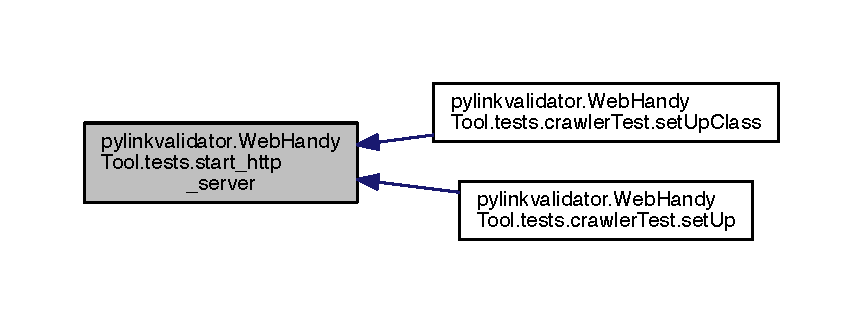
\includegraphics[width=350pt]{namespacepylinkvalidator_1_1_web_handy_tool_1_1tests_a9db60e3a111b5405bdfbc14fecaf488d_icgraph}
\end{center}
\end{figure}




\subsection{Variable Documentation}
\index{pylinkvalidator\+::\+Web\+Handy\+Tool\+::tests@{pylinkvalidator\+::\+Web\+Handy\+Tool\+::tests}!crawl\+Test\+Suite@{crawl\+Test\+Suite}}
\index{crawl\+Test\+Suite@{crawl\+Test\+Suite}!pylinkvalidator\+::\+Web\+Handy\+Tool\+::tests@{pylinkvalidator\+::\+Web\+Handy\+Tool\+::tests}}
\subsubsection[{crawl\+Test\+Suite}]{\setlength{\rightskip}{0pt plus 5cm}tuple pylinkvalidator.\+Web\+Handy\+Tool.\+tests.\+crawl\+Test\+Suite = unittest.\+Test\+Loader()}\hypertarget{namespacepylinkvalidator_1_1_web_handy_tool_1_1tests_a151ef06220ff5cd22210deb3f5c38a1f}{}\label{namespacepylinkvalidator_1_1_web_handy_tool_1_1tests_a151ef06220ff5cd22210deb3f5c38a1f}
\index{pylinkvalidator\+::\+Web\+Handy\+Tool\+::tests@{pylinkvalidator\+::\+Web\+Handy\+Tool\+::tests}!search\+Test\+Suite@{search\+Test\+Suite}}
\index{search\+Test\+Suite@{search\+Test\+Suite}!pylinkvalidator\+::\+Web\+Handy\+Tool\+::tests@{pylinkvalidator\+::\+Web\+Handy\+Tool\+::tests}}
\subsubsection[{search\+Test\+Suite}]{\setlength{\rightskip}{0pt plus 5cm}tuple pylinkvalidator.\+Web\+Handy\+Tool.\+tests.\+search\+Test\+Suite = unittest.\+Test\+Loader()}\hypertarget{namespacepylinkvalidator_1_1_web_handy_tool_1_1tests_a2e5e49f77bf2a9ce392f59a9bee51808}{}\label{namespacepylinkvalidator_1_1_web_handy_tool_1_1tests_a2e5e49f77bf2a9ce392f59a9bee51808}
\index{pylinkvalidator\+::\+Web\+Handy\+Tool\+::tests@{pylinkvalidator\+::\+Web\+Handy\+Tool\+::tests}!T\+E\+S\+T\+\_\+\+F\+I\+L\+E\+S\+\_\+\+D\+IR@{T\+E\+S\+T\+\_\+\+F\+I\+L\+E\+S\+\_\+\+D\+IR}}
\index{T\+E\+S\+T\+\_\+\+F\+I\+L\+E\+S\+\_\+\+D\+IR@{T\+E\+S\+T\+\_\+\+F\+I\+L\+E\+S\+\_\+\+D\+IR}!pylinkvalidator\+::\+Web\+Handy\+Tool\+::tests@{pylinkvalidator\+::\+Web\+Handy\+Tool\+::tests}}
\subsubsection[{T\+E\+S\+T\+\_\+\+F\+I\+L\+E\+S\+\_\+\+D\+IR}]{\setlength{\rightskip}{0pt plus 5cm}tuple pylinkvalidator.\+Web\+Handy\+Tool.\+tests.\+T\+E\+S\+T\+\_\+\+F\+I\+L\+E\+S\+\_\+\+D\+IR}\hypertarget{namespacepylinkvalidator_1_1_web_handy_tool_1_1tests_a14166a02e5bd8dca477698e70415a8dd}{}\label{namespacepylinkvalidator_1_1_web_handy_tool_1_1tests_a14166a02e5bd8dca477698e70415a8dd}
{\bfseries Initial value\+:}
\begin{DoxyCode}
1 = os.path.join(os.path.dirname(os.path.realpath(\_\_file\_\_)),
2                               \textcolor{stringliteral}{'testfiles'})
\end{DoxyCode}
\index{pylinkvalidator\+::\+Web\+Handy\+Tool\+::tests@{pylinkvalidator\+::\+Web\+Handy\+Tool\+::tests}!url\+Test\+Suite@{url\+Test\+Suite}}
\index{url\+Test\+Suite@{url\+Test\+Suite}!pylinkvalidator\+::\+Web\+Handy\+Tool\+::tests@{pylinkvalidator\+::\+Web\+Handy\+Tool\+::tests}}
\subsubsection[{url\+Test\+Suite}]{\setlength{\rightskip}{0pt plus 5cm}tuple pylinkvalidator.\+Web\+Handy\+Tool.\+tests.\+url\+Test\+Suite = unittest.\+Test\+Loader()}\hypertarget{namespacepylinkvalidator_1_1_web_handy_tool_1_1tests_acf8bf6dfdff5780f67938a68973a60c8}{}\label{namespacepylinkvalidator_1_1_web_handy_tool_1_1tests_acf8bf6dfdff5780f67938a68973a60c8}

\hypertarget{namespacepylinkvalidator_1_1_web_handy_tool_1_1url_corrector}{}\section{pylinkvalidator.\+Web\+Handy\+Tool.\+url\+Corrector Namespace Reference}
\label{namespacepylinkvalidator_1_1_web_handy_tool_1_1url_corrector}\index{pylinkvalidator.\+Web\+Handy\+Tool.\+url\+Corrector@{pylinkvalidator.\+Web\+Handy\+Tool.\+url\+Corrector}}
\subsection*{Classes}
\begin{DoxyCompactItemize}
\item 
class \hyperlink{classpylinkvalidator_1_1_web_handy_tool_1_1url_corrector_1_1_h_t_m_l__corrector__help}{H\+T\+M\+L\+\_\+corrector\+\_\+help}
\item 
class \hyperlink{classpylinkvalidator_1_1_web_handy_tool_1_1url_corrector_1_1url_corrector}{url\+Corrector}
\end{DoxyCompactItemize}

\hypertarget{namespacepylinkvalidator_1_1_web_handy_tool_1_1_web___crawler}{}\section{pylinkvalidator.\+Web\+Handy\+Tool.\+Web\+\_\+\+Crawler Namespace Reference}
\label{namespacepylinkvalidator_1_1_web_handy_tool_1_1_web___crawler}\index{pylinkvalidator.\+Web\+Handy\+Tool.\+Web\+\_\+\+Crawler@{pylinkvalidator.\+Web\+Handy\+Tool.\+Web\+\_\+\+Crawler}}
\subsection*{Classes}
\begin{DoxyCompactItemize}
\item 
class \hyperlink{classpylinkvalidator_1_1_web_handy_tool_1_1_web___crawler_1_1_web___crawler}{Web\+\_\+\+Crawler}
\end{DoxyCompactItemize}
\subsection*{Variables}
\begin{DoxyCompactItemize}
\item 
string \hyperlink{namespacepylinkvalidator_1_1_web_handy_tool_1_1_web___crawler_affb3151f3f1a14a483da5ff3c2c148cf}{\+\_\+\+\_\+author\+\_\+\+\_\+} = \textquotesingle{}Abe\textquotesingle{}
\item 
tuple \hyperlink{namespacepylinkvalidator_1_1_web_handy_tool_1_1_web___crawler_a3b4c79fe9756714e1b12573b644499bc}{crawler} = \hyperlink{classpylinkvalidator_1_1_web_handy_tool_1_1_web___crawler_1_1_web___crawler}{Web\+\_\+\+Crawler}()
\item 
tuple \hyperlink{namespacepylinkvalidator_1_1_web_handy_tool_1_1_web___crawler_a51cc3473f0ab9b1254af83e5559b129e}{option} = crawler.\+option()
\end{DoxyCompactItemize}


\subsection{Variable Documentation}
\index{pylinkvalidator\+::\+Web\+Handy\+Tool\+::\+Web\+\_\+\+Crawler@{pylinkvalidator\+::\+Web\+Handy\+Tool\+::\+Web\+\_\+\+Crawler}!\+\_\+\+\_\+author\+\_\+\+\_\+@{\+\_\+\+\_\+author\+\_\+\+\_\+}}
\index{\+\_\+\+\_\+author\+\_\+\+\_\+@{\+\_\+\+\_\+author\+\_\+\+\_\+}!pylinkvalidator\+::\+Web\+Handy\+Tool\+::\+Web\+\_\+\+Crawler@{pylinkvalidator\+::\+Web\+Handy\+Tool\+::\+Web\+\_\+\+Crawler}}
\subsubsection[{\+\_\+\+\_\+author\+\_\+\+\_\+}]{\setlength{\rightskip}{0pt plus 5cm}string pylinkvalidator.\+Web\+Handy\+Tool.\+Web\+\_\+\+Crawler.\+\_\+\+\_\+author\+\_\+\+\_\+ = \textquotesingle{}Abe\textquotesingle{}}\hypertarget{namespacepylinkvalidator_1_1_web_handy_tool_1_1_web___crawler_affb3151f3f1a14a483da5ff3c2c148cf}{}\label{namespacepylinkvalidator_1_1_web_handy_tool_1_1_web___crawler_affb3151f3f1a14a483da5ff3c2c148cf}
\index{pylinkvalidator\+::\+Web\+Handy\+Tool\+::\+Web\+\_\+\+Crawler@{pylinkvalidator\+::\+Web\+Handy\+Tool\+::\+Web\+\_\+\+Crawler}!crawler@{crawler}}
\index{crawler@{crawler}!pylinkvalidator\+::\+Web\+Handy\+Tool\+::\+Web\+\_\+\+Crawler@{pylinkvalidator\+::\+Web\+Handy\+Tool\+::\+Web\+\_\+\+Crawler}}
\subsubsection[{crawler}]{\setlength{\rightskip}{0pt plus 5cm}tuple pylinkvalidator.\+Web\+Handy\+Tool.\+Web\+\_\+\+Crawler.\+crawler = {\bf Web\+\_\+\+Crawler}()}\hypertarget{namespacepylinkvalidator_1_1_web_handy_tool_1_1_web___crawler_a3b4c79fe9756714e1b12573b644499bc}{}\label{namespacepylinkvalidator_1_1_web_handy_tool_1_1_web___crawler_a3b4c79fe9756714e1b12573b644499bc}
\index{pylinkvalidator\+::\+Web\+Handy\+Tool\+::\+Web\+\_\+\+Crawler@{pylinkvalidator\+::\+Web\+Handy\+Tool\+::\+Web\+\_\+\+Crawler}!option@{option}}
\index{option@{option}!pylinkvalidator\+::\+Web\+Handy\+Tool\+::\+Web\+\_\+\+Crawler@{pylinkvalidator\+::\+Web\+Handy\+Tool\+::\+Web\+\_\+\+Crawler}}
\subsubsection[{option}]{\setlength{\rightskip}{0pt plus 5cm}tuple pylinkvalidator.\+Web\+Handy\+Tool.\+Web\+\_\+\+Crawler.\+option = crawler.\+option()}\hypertarget{namespacepylinkvalidator_1_1_web_handy_tool_1_1_web___crawler_a51cc3473f0ab9b1254af83e5559b129e}{}\label{namespacepylinkvalidator_1_1_web_handy_tool_1_1_web___crawler_a51cc3473f0ab9b1254af83e5559b129e}

\hypertarget{namespace_test_string}{}\section{Test\+String Namespace Reference}
\label{namespace_test_string}\index{Test\+String@{Test\+String}}
\subsection*{Classes}
\begin{DoxyCompactItemize}
\item 
class \hyperlink{class_test_string_1_1_test_string_methods}{Test\+String\+Methods}
\end{DoxyCompactItemize}

\chapter{Class Documentation}
\hypertarget{classpylinkvalidator_1_1_web_handy_tool_1_1tests_1_1crawler_test}{}\section{pylinkvalidator.\+Web\+Handy\+Tool.\+tests.\+crawler\+Test Class Reference}
\label{classpylinkvalidator_1_1_web_handy_tool_1_1tests_1_1crawler_test}\index{pylinkvalidator.\+Web\+Handy\+Tool.\+tests.\+crawler\+Test@{pylinkvalidator.\+Web\+Handy\+Tool.\+tests.\+crawler\+Test}}


Inheritance diagram for pylinkvalidator.\+Web\+Handy\+Tool.\+tests.\+crawler\+Test\+:
\nopagebreak
\begin{figure}[H]
\begin{center}
\leavevmode
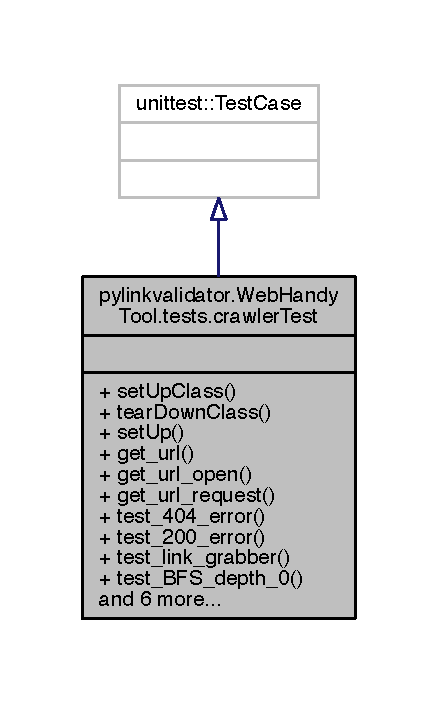
\includegraphics[width=210pt]{classpylinkvalidator_1_1_web_handy_tool_1_1tests_1_1crawler_test__inherit__graph}
\end{center}
\end{figure}


Collaboration diagram for pylinkvalidator.\+Web\+Handy\+Tool.\+tests.\+crawler\+Test\+:
\nopagebreak
\begin{figure}[H]
\begin{center}
\leavevmode
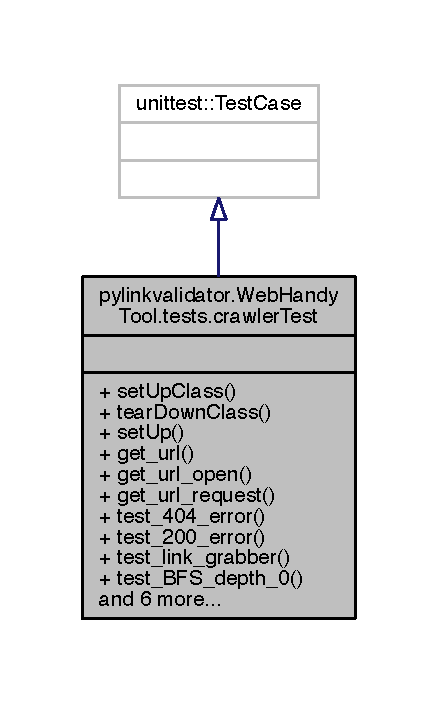
\includegraphics[width=210pt]{classpylinkvalidator_1_1_web_handy_tool_1_1tests_1_1crawler_test__coll__graph}
\end{center}
\end{figure}
\subsection*{Public Member Functions}
\begin{DoxyCompactItemize}
\item 
def \hyperlink{classpylinkvalidator_1_1_web_handy_tool_1_1tests_1_1crawler_test_a488a0ba0983f998e70b16f99d1206a4e}{set\+Up\+Class} (cls)
\item 
def \hyperlink{classpylinkvalidator_1_1_web_handy_tool_1_1tests_1_1crawler_test_af6eb886ff5b26bd69f9f309ce3d84981}{tear\+Down\+Class} (cls)
\item 
def \hyperlink{classpylinkvalidator_1_1_web_handy_tool_1_1tests_1_1crawler_test_a59924a9695a61c66650b7c4c3a5697cc}{set\+Up} (self)
\item 
def \hyperlink{classpylinkvalidator_1_1_web_handy_tool_1_1tests_1_1crawler_test_a9bfdb2427ff25ed415115347baa183e3}{get\+\_\+url} (self, test\+\_\+url)
\item 
def \hyperlink{classpylinkvalidator_1_1_web_handy_tool_1_1tests_1_1crawler_test_a3db5e9ca3315af5e2b8f29c098667a9d}{get\+\_\+url\+\_\+open} (self)
\item 
def \hyperlink{classpylinkvalidator_1_1_web_handy_tool_1_1tests_1_1crawler_test_a16539cd0e3add6d4ec5557194a96c0bc}{get\+\_\+url\+\_\+request} (self)
\item 
def \hyperlink{classpylinkvalidator_1_1_web_handy_tool_1_1tests_1_1crawler_test_a404f44c124831e5c9593b2b3ebc6be88}{test\+\_\+404\+\_\+error} (self)
\item 
def \hyperlink{classpylinkvalidator_1_1_web_handy_tool_1_1tests_1_1crawler_test_adb2a22bd6d79bc38b353d966d9a2b45f}{test\+\_\+200\+\_\+error} (self)
\item 
def \hyperlink{classpylinkvalidator_1_1_web_handy_tool_1_1tests_1_1crawler_test_ac00856c89d2d4130ffe0ca385df3f679}{test\+\_\+link\+\_\+grabber} (self)
\item 
def \hyperlink{classpylinkvalidator_1_1_web_handy_tool_1_1tests_1_1crawler_test_a48e6e241f7fa3ceaa7c49675292c8218}{test\+\_\+\+B\+F\+S\+\_\+depth\+\_\+0} (self)
\item 
def \hyperlink{classpylinkvalidator_1_1_web_handy_tool_1_1tests_1_1crawler_test_acde5a29e709f738a357da43e8ce8e06b}{test\+\_\+\+B\+F\+S\+\_\+depth\+\_\+1} (self)
\item 
def \hyperlink{classpylinkvalidator_1_1_web_handy_tool_1_1tests_1_1crawler_test_abb5fe183951e209f66c2b4e292c99eb7}{test\+\_\+\+B\+F\+S\+\_\+depth\+\_\+2} (self)
\item 
def \hyperlink{classpylinkvalidator_1_1_web_handy_tool_1_1tests_1_1crawler_test_a92c82295f6e332a249a11868f5999218}{test\+\_\+\+B\+F\+S\+\_\+depth\+\_\+3} (self)
\item 
def \hyperlink{classpylinkvalidator_1_1_web_handy_tool_1_1tests_1_1crawler_test_a433365f3474025469ab42635234cbef0}{test\+\_\+\+B\+F\+S\+\_\+depth\+\_\+4} (self)
\item 
def \hyperlink{classpylinkvalidator_1_1_web_handy_tool_1_1tests_1_1crawler_test_a96a6738fbd35cf6397c417d262dd30f0}{test\+\_\+\+B\+F\+S\+\_\+depth\+\_\+5} (self)
\item 
def \hyperlink{classpylinkvalidator_1_1_web_handy_tool_1_1tests_1_1crawler_test_a4f86d42852e498de1c0d70b11c8950a1}{test\+\_\+download} (self)
\end{DoxyCompactItemize}


\subsection{Member Function Documentation}
\index{pylinkvalidator\+::\+Web\+Handy\+Tool\+::tests\+::crawler\+Test@{pylinkvalidator\+::\+Web\+Handy\+Tool\+::tests\+::crawler\+Test}!get\+\_\+url@{get\+\_\+url}}
\index{get\+\_\+url@{get\+\_\+url}!pylinkvalidator\+::\+Web\+Handy\+Tool\+::tests\+::crawler\+Test@{pylinkvalidator\+::\+Web\+Handy\+Tool\+::tests\+::crawler\+Test}}
\subsubsection[{get\+\_\+url(self, test\+\_\+url)}]{\setlength{\rightskip}{0pt plus 5cm}def pylinkvalidator.\+Web\+Handy\+Tool.\+tests.\+crawler\+Test.\+get\+\_\+url (
\begin{DoxyParamCaption}
\item[{}]{self, }
\item[{}]{test\+\_\+url}
\end{DoxyParamCaption}
)}\hypertarget{classpylinkvalidator_1_1_web_handy_tool_1_1tests_1_1crawler_test_a9bfdb2427ff25ed415115347baa183e3}{}\label{classpylinkvalidator_1_1_web_handy_tool_1_1tests_1_1crawler_test_a9bfdb2427ff25ed415115347baa183e3}


Here is the caller graph for this function\+:
\nopagebreak
\begin{figure}[H]
\begin{center}
\leavevmode
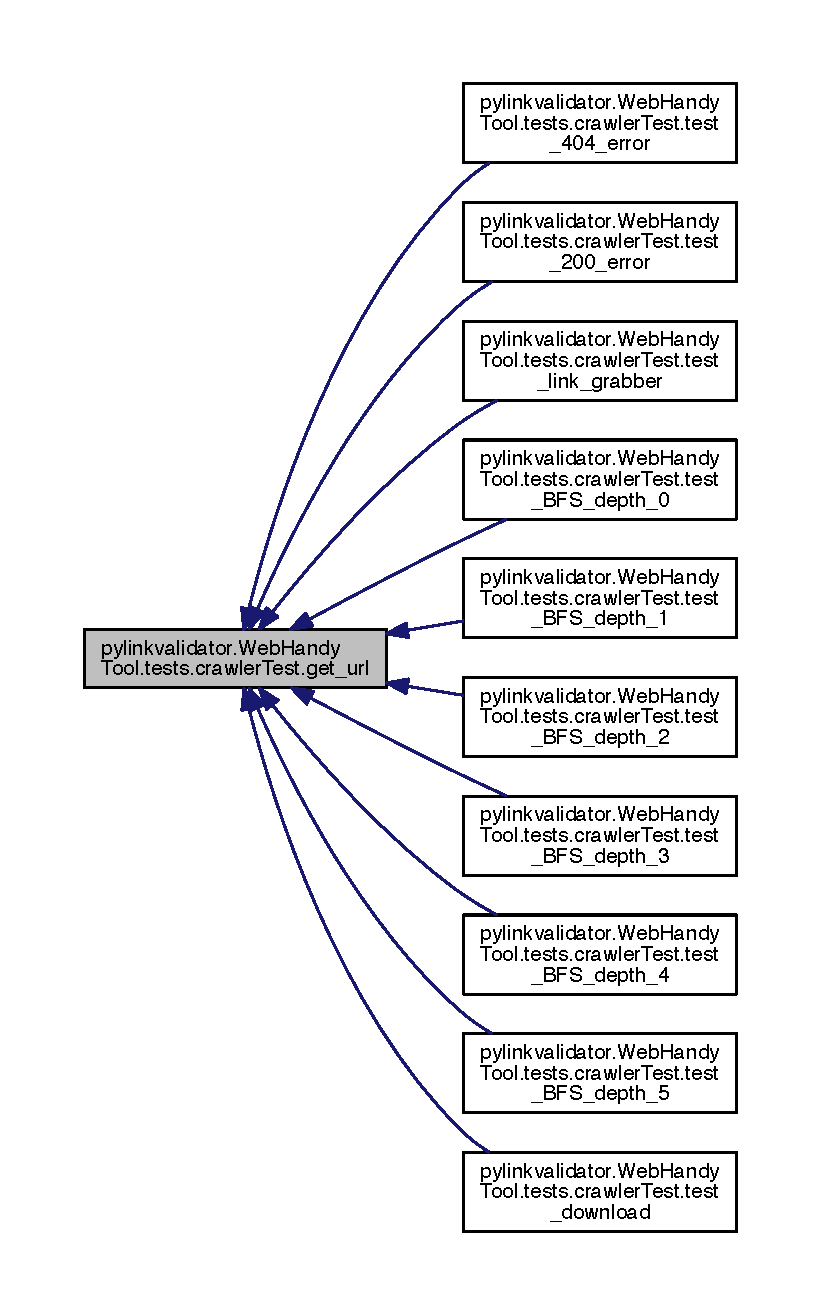
\includegraphics[height=550pt]{classpylinkvalidator_1_1_web_handy_tool_1_1tests_1_1crawler_test_a9bfdb2427ff25ed415115347baa183e3_icgraph}
\end{center}
\end{figure}


\index{pylinkvalidator\+::\+Web\+Handy\+Tool\+::tests\+::crawler\+Test@{pylinkvalidator\+::\+Web\+Handy\+Tool\+::tests\+::crawler\+Test}!get\+\_\+url\+\_\+open@{get\+\_\+url\+\_\+open}}
\index{get\+\_\+url\+\_\+open@{get\+\_\+url\+\_\+open}!pylinkvalidator\+::\+Web\+Handy\+Tool\+::tests\+::crawler\+Test@{pylinkvalidator\+::\+Web\+Handy\+Tool\+::tests\+::crawler\+Test}}
\subsubsection[{get\+\_\+url\+\_\+open(self)}]{\setlength{\rightskip}{0pt plus 5cm}def pylinkvalidator.\+Web\+Handy\+Tool.\+tests.\+crawler\+Test.\+get\+\_\+url\+\_\+open (
\begin{DoxyParamCaption}
\item[{}]{self}
\end{DoxyParamCaption}
)}\hypertarget{classpylinkvalidator_1_1_web_handy_tool_1_1tests_1_1crawler_test_a3db5e9ca3315af5e2b8f29c098667a9d}{}\label{classpylinkvalidator_1_1_web_handy_tool_1_1tests_1_1crawler_test_a3db5e9ca3315af5e2b8f29c098667a9d}


Here is the caller graph for this function\+:
\nopagebreak
\begin{figure}[H]
\begin{center}
\leavevmode
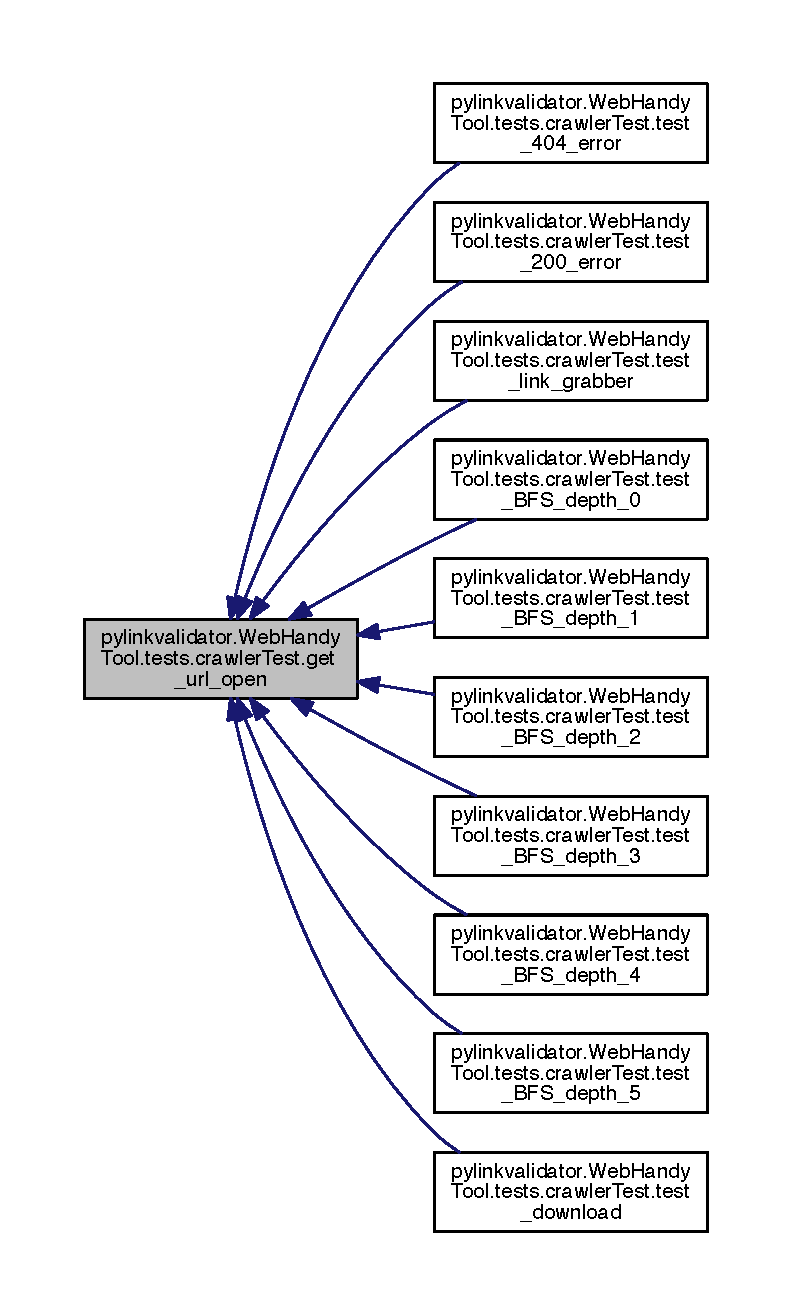
\includegraphics[height=550pt]{classpylinkvalidator_1_1_web_handy_tool_1_1tests_1_1crawler_test_a3db5e9ca3315af5e2b8f29c098667a9d_icgraph}
\end{center}
\end{figure}


\index{pylinkvalidator\+::\+Web\+Handy\+Tool\+::tests\+::crawler\+Test@{pylinkvalidator\+::\+Web\+Handy\+Tool\+::tests\+::crawler\+Test}!get\+\_\+url\+\_\+request@{get\+\_\+url\+\_\+request}}
\index{get\+\_\+url\+\_\+request@{get\+\_\+url\+\_\+request}!pylinkvalidator\+::\+Web\+Handy\+Tool\+::tests\+::crawler\+Test@{pylinkvalidator\+::\+Web\+Handy\+Tool\+::tests\+::crawler\+Test}}
\subsubsection[{get\+\_\+url\+\_\+request(self)}]{\setlength{\rightskip}{0pt plus 5cm}def pylinkvalidator.\+Web\+Handy\+Tool.\+tests.\+crawler\+Test.\+get\+\_\+url\+\_\+request (
\begin{DoxyParamCaption}
\item[{}]{self}
\end{DoxyParamCaption}
)}\hypertarget{classpylinkvalidator_1_1_web_handy_tool_1_1tests_1_1crawler_test_a16539cd0e3add6d4ec5557194a96c0bc}{}\label{classpylinkvalidator_1_1_web_handy_tool_1_1tests_1_1crawler_test_a16539cd0e3add6d4ec5557194a96c0bc}
\index{pylinkvalidator\+::\+Web\+Handy\+Tool\+::tests\+::crawler\+Test@{pylinkvalidator\+::\+Web\+Handy\+Tool\+::tests\+::crawler\+Test}!set\+Up@{set\+Up}}
\index{set\+Up@{set\+Up}!pylinkvalidator\+::\+Web\+Handy\+Tool\+::tests\+::crawler\+Test@{pylinkvalidator\+::\+Web\+Handy\+Tool\+::tests\+::crawler\+Test}}
\subsubsection[{set\+Up(self)}]{\setlength{\rightskip}{0pt plus 5cm}def pylinkvalidator.\+Web\+Handy\+Tool.\+tests.\+crawler\+Test.\+set\+Up (
\begin{DoxyParamCaption}
\item[{}]{self}
\end{DoxyParamCaption}
)}\hypertarget{classpylinkvalidator_1_1_web_handy_tool_1_1tests_1_1crawler_test_a59924a9695a61c66650b7c4c3a5697cc}{}\label{classpylinkvalidator_1_1_web_handy_tool_1_1tests_1_1crawler_test_a59924a9695a61c66650b7c4c3a5697cc}


Here is the call graph for this function\+:
\nopagebreak
\begin{figure}[H]
\begin{center}
\leavevmode
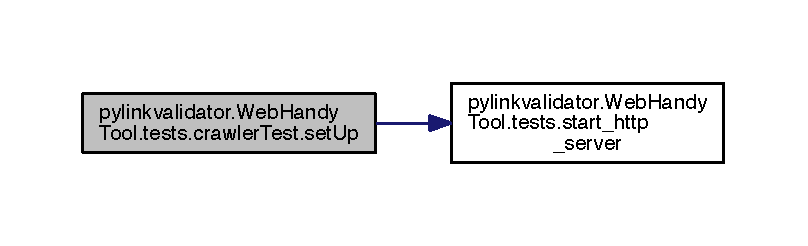
\includegraphics[width=350pt]{classpylinkvalidator_1_1_web_handy_tool_1_1tests_1_1crawler_test_a59924a9695a61c66650b7c4c3a5697cc_cgraph}
\end{center}
\end{figure}


\index{pylinkvalidator\+::\+Web\+Handy\+Tool\+::tests\+::crawler\+Test@{pylinkvalidator\+::\+Web\+Handy\+Tool\+::tests\+::crawler\+Test}!set\+Up\+Class@{set\+Up\+Class}}
\index{set\+Up\+Class@{set\+Up\+Class}!pylinkvalidator\+::\+Web\+Handy\+Tool\+::tests\+::crawler\+Test@{pylinkvalidator\+::\+Web\+Handy\+Tool\+::tests\+::crawler\+Test}}
\subsubsection[{set\+Up\+Class(cls)}]{\setlength{\rightskip}{0pt plus 5cm}def pylinkvalidator.\+Web\+Handy\+Tool.\+tests.\+crawler\+Test.\+set\+Up\+Class (
\begin{DoxyParamCaption}
\item[{}]{cls}
\end{DoxyParamCaption}
)}\hypertarget{classpylinkvalidator_1_1_web_handy_tool_1_1tests_1_1crawler_test_a488a0ba0983f998e70b16f99d1206a4e}{}\label{classpylinkvalidator_1_1_web_handy_tool_1_1tests_1_1crawler_test_a488a0ba0983f998e70b16f99d1206a4e}


Here is the call graph for this function\+:
\nopagebreak
\begin{figure}[H]
\begin{center}
\leavevmode
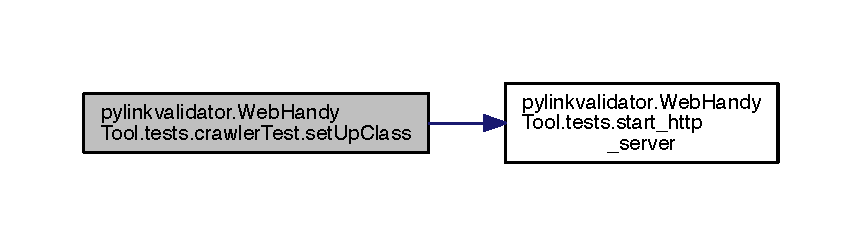
\includegraphics[width=350pt]{classpylinkvalidator_1_1_web_handy_tool_1_1tests_1_1crawler_test_a488a0ba0983f998e70b16f99d1206a4e_cgraph}
\end{center}
\end{figure}


\index{pylinkvalidator\+::\+Web\+Handy\+Tool\+::tests\+::crawler\+Test@{pylinkvalidator\+::\+Web\+Handy\+Tool\+::tests\+::crawler\+Test}!tear\+Down\+Class@{tear\+Down\+Class}}
\index{tear\+Down\+Class@{tear\+Down\+Class}!pylinkvalidator\+::\+Web\+Handy\+Tool\+::tests\+::crawler\+Test@{pylinkvalidator\+::\+Web\+Handy\+Tool\+::tests\+::crawler\+Test}}
\subsubsection[{tear\+Down\+Class(cls)}]{\setlength{\rightskip}{0pt plus 5cm}def pylinkvalidator.\+Web\+Handy\+Tool.\+tests.\+crawler\+Test.\+tear\+Down\+Class (
\begin{DoxyParamCaption}
\item[{}]{cls}
\end{DoxyParamCaption}
)}\hypertarget{classpylinkvalidator_1_1_web_handy_tool_1_1tests_1_1crawler_test_af6eb886ff5b26bd69f9f309ce3d84981}{}\label{classpylinkvalidator_1_1_web_handy_tool_1_1tests_1_1crawler_test_af6eb886ff5b26bd69f9f309ce3d84981}
\index{pylinkvalidator\+::\+Web\+Handy\+Tool\+::tests\+::crawler\+Test@{pylinkvalidator\+::\+Web\+Handy\+Tool\+::tests\+::crawler\+Test}!test\+\_\+200\+\_\+error@{test\+\_\+200\+\_\+error}}
\index{test\+\_\+200\+\_\+error@{test\+\_\+200\+\_\+error}!pylinkvalidator\+::\+Web\+Handy\+Tool\+::tests\+::crawler\+Test@{pylinkvalidator\+::\+Web\+Handy\+Tool\+::tests\+::crawler\+Test}}
\subsubsection[{test\+\_\+200\+\_\+error(self)}]{\setlength{\rightskip}{0pt plus 5cm}def pylinkvalidator.\+Web\+Handy\+Tool.\+tests.\+crawler\+Test.\+test\+\_\+200\+\_\+error (
\begin{DoxyParamCaption}
\item[{}]{self}
\end{DoxyParamCaption}
)}\hypertarget{classpylinkvalidator_1_1_web_handy_tool_1_1tests_1_1crawler_test_adb2a22bd6d79bc38b353d966d9a2b45f}{}\label{classpylinkvalidator_1_1_web_handy_tool_1_1tests_1_1crawler_test_adb2a22bd6d79bc38b353d966d9a2b45f}


Here is the call graph for this function\+:
\nopagebreak
\begin{figure}[H]
\begin{center}
\leavevmode
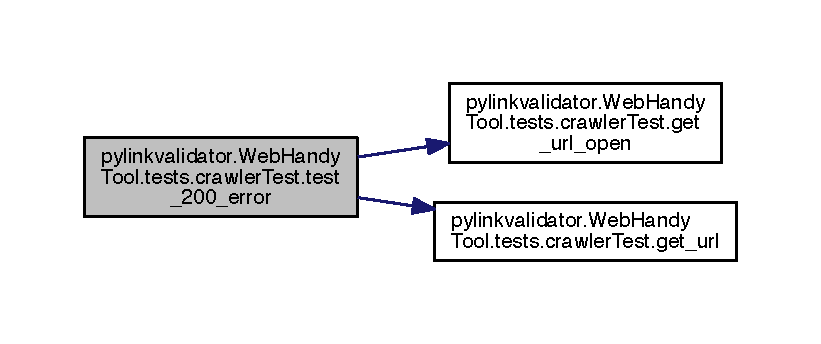
\includegraphics[width=350pt]{classpylinkvalidator_1_1_web_handy_tool_1_1tests_1_1crawler_test_adb2a22bd6d79bc38b353d966d9a2b45f_cgraph}
\end{center}
\end{figure}


\index{pylinkvalidator\+::\+Web\+Handy\+Tool\+::tests\+::crawler\+Test@{pylinkvalidator\+::\+Web\+Handy\+Tool\+::tests\+::crawler\+Test}!test\+\_\+404\+\_\+error@{test\+\_\+404\+\_\+error}}
\index{test\+\_\+404\+\_\+error@{test\+\_\+404\+\_\+error}!pylinkvalidator\+::\+Web\+Handy\+Tool\+::tests\+::crawler\+Test@{pylinkvalidator\+::\+Web\+Handy\+Tool\+::tests\+::crawler\+Test}}
\subsubsection[{test\+\_\+404\+\_\+error(self)}]{\setlength{\rightskip}{0pt plus 5cm}def pylinkvalidator.\+Web\+Handy\+Tool.\+tests.\+crawler\+Test.\+test\+\_\+404\+\_\+error (
\begin{DoxyParamCaption}
\item[{}]{self}
\end{DoxyParamCaption}
)}\hypertarget{classpylinkvalidator_1_1_web_handy_tool_1_1tests_1_1crawler_test_a404f44c124831e5c9593b2b3ebc6be88}{}\label{classpylinkvalidator_1_1_web_handy_tool_1_1tests_1_1crawler_test_a404f44c124831e5c9593b2b3ebc6be88}


Here is the call graph for this function\+:
\nopagebreak
\begin{figure}[H]
\begin{center}
\leavevmode
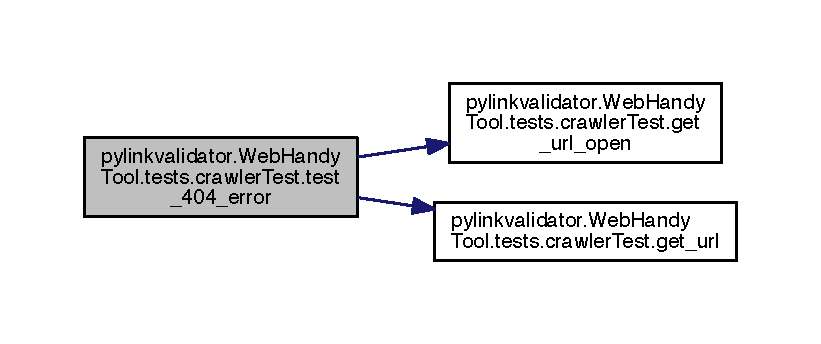
\includegraphics[width=350pt]{classpylinkvalidator_1_1_web_handy_tool_1_1tests_1_1crawler_test_a404f44c124831e5c9593b2b3ebc6be88_cgraph}
\end{center}
\end{figure}


\index{pylinkvalidator\+::\+Web\+Handy\+Tool\+::tests\+::crawler\+Test@{pylinkvalidator\+::\+Web\+Handy\+Tool\+::tests\+::crawler\+Test}!test\+\_\+\+B\+F\+S\+\_\+depth\+\_\+0@{test\+\_\+\+B\+F\+S\+\_\+depth\+\_\+0}}
\index{test\+\_\+\+B\+F\+S\+\_\+depth\+\_\+0@{test\+\_\+\+B\+F\+S\+\_\+depth\+\_\+0}!pylinkvalidator\+::\+Web\+Handy\+Tool\+::tests\+::crawler\+Test@{pylinkvalidator\+::\+Web\+Handy\+Tool\+::tests\+::crawler\+Test}}
\subsubsection[{test\+\_\+\+B\+F\+S\+\_\+depth\+\_\+0(self)}]{\setlength{\rightskip}{0pt plus 5cm}def pylinkvalidator.\+Web\+Handy\+Tool.\+tests.\+crawler\+Test.\+test\+\_\+\+B\+F\+S\+\_\+depth\+\_\+0 (
\begin{DoxyParamCaption}
\item[{}]{self}
\end{DoxyParamCaption}
)}\hypertarget{classpylinkvalidator_1_1_web_handy_tool_1_1tests_1_1crawler_test_a48e6e241f7fa3ceaa7c49675292c8218}{}\label{classpylinkvalidator_1_1_web_handy_tool_1_1tests_1_1crawler_test_a48e6e241f7fa3ceaa7c49675292c8218}


Here is the call graph for this function\+:
\nopagebreak
\begin{figure}[H]
\begin{center}
\leavevmode
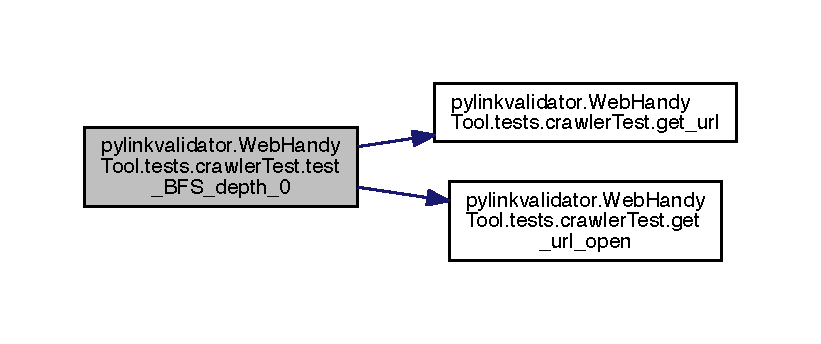
\includegraphics[width=350pt]{classpylinkvalidator_1_1_web_handy_tool_1_1tests_1_1crawler_test_a48e6e241f7fa3ceaa7c49675292c8218_cgraph}
\end{center}
\end{figure}


\index{pylinkvalidator\+::\+Web\+Handy\+Tool\+::tests\+::crawler\+Test@{pylinkvalidator\+::\+Web\+Handy\+Tool\+::tests\+::crawler\+Test}!test\+\_\+\+B\+F\+S\+\_\+depth\+\_\+1@{test\+\_\+\+B\+F\+S\+\_\+depth\+\_\+1}}
\index{test\+\_\+\+B\+F\+S\+\_\+depth\+\_\+1@{test\+\_\+\+B\+F\+S\+\_\+depth\+\_\+1}!pylinkvalidator\+::\+Web\+Handy\+Tool\+::tests\+::crawler\+Test@{pylinkvalidator\+::\+Web\+Handy\+Tool\+::tests\+::crawler\+Test}}
\subsubsection[{test\+\_\+\+B\+F\+S\+\_\+depth\+\_\+1(self)}]{\setlength{\rightskip}{0pt plus 5cm}def pylinkvalidator.\+Web\+Handy\+Tool.\+tests.\+crawler\+Test.\+test\+\_\+\+B\+F\+S\+\_\+depth\+\_\+1 (
\begin{DoxyParamCaption}
\item[{}]{self}
\end{DoxyParamCaption}
)}\hypertarget{classpylinkvalidator_1_1_web_handy_tool_1_1tests_1_1crawler_test_acde5a29e709f738a357da43e8ce8e06b}{}\label{classpylinkvalidator_1_1_web_handy_tool_1_1tests_1_1crawler_test_acde5a29e709f738a357da43e8ce8e06b}


Here is the call graph for this function\+:
\nopagebreak
\begin{figure}[H]
\begin{center}
\leavevmode
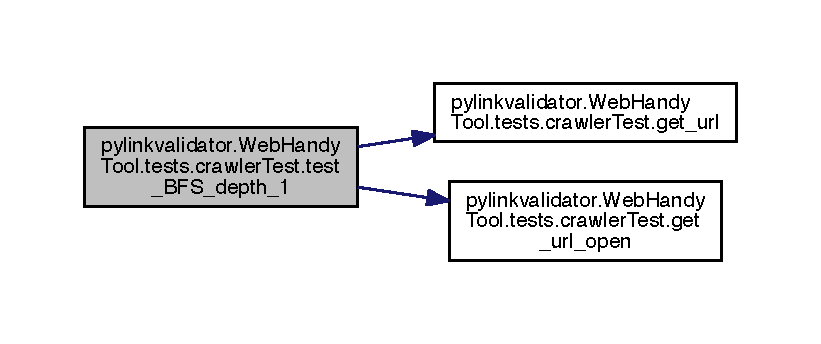
\includegraphics[width=350pt]{classpylinkvalidator_1_1_web_handy_tool_1_1tests_1_1crawler_test_acde5a29e709f738a357da43e8ce8e06b_cgraph}
\end{center}
\end{figure}


\index{pylinkvalidator\+::\+Web\+Handy\+Tool\+::tests\+::crawler\+Test@{pylinkvalidator\+::\+Web\+Handy\+Tool\+::tests\+::crawler\+Test}!test\+\_\+\+B\+F\+S\+\_\+depth\+\_\+2@{test\+\_\+\+B\+F\+S\+\_\+depth\+\_\+2}}
\index{test\+\_\+\+B\+F\+S\+\_\+depth\+\_\+2@{test\+\_\+\+B\+F\+S\+\_\+depth\+\_\+2}!pylinkvalidator\+::\+Web\+Handy\+Tool\+::tests\+::crawler\+Test@{pylinkvalidator\+::\+Web\+Handy\+Tool\+::tests\+::crawler\+Test}}
\subsubsection[{test\+\_\+\+B\+F\+S\+\_\+depth\+\_\+2(self)}]{\setlength{\rightskip}{0pt plus 5cm}def pylinkvalidator.\+Web\+Handy\+Tool.\+tests.\+crawler\+Test.\+test\+\_\+\+B\+F\+S\+\_\+depth\+\_\+2 (
\begin{DoxyParamCaption}
\item[{}]{self}
\end{DoxyParamCaption}
)}\hypertarget{classpylinkvalidator_1_1_web_handy_tool_1_1tests_1_1crawler_test_abb5fe183951e209f66c2b4e292c99eb7}{}\label{classpylinkvalidator_1_1_web_handy_tool_1_1tests_1_1crawler_test_abb5fe183951e209f66c2b4e292c99eb7}


Here is the call graph for this function\+:
\nopagebreak
\begin{figure}[H]
\begin{center}
\leavevmode
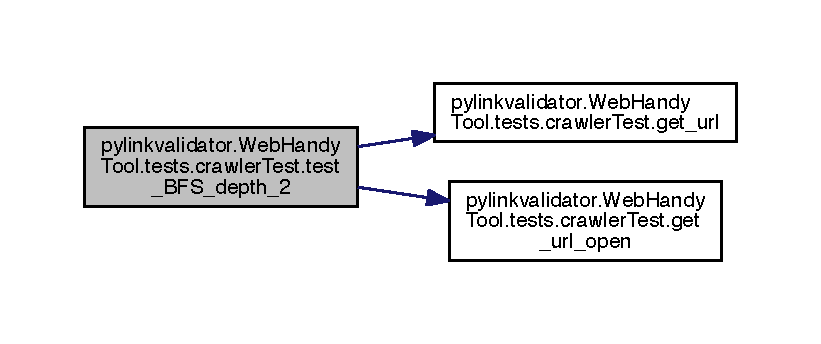
\includegraphics[width=350pt]{classpylinkvalidator_1_1_web_handy_tool_1_1tests_1_1crawler_test_abb5fe183951e209f66c2b4e292c99eb7_cgraph}
\end{center}
\end{figure}


\index{pylinkvalidator\+::\+Web\+Handy\+Tool\+::tests\+::crawler\+Test@{pylinkvalidator\+::\+Web\+Handy\+Tool\+::tests\+::crawler\+Test}!test\+\_\+\+B\+F\+S\+\_\+depth\+\_\+3@{test\+\_\+\+B\+F\+S\+\_\+depth\+\_\+3}}
\index{test\+\_\+\+B\+F\+S\+\_\+depth\+\_\+3@{test\+\_\+\+B\+F\+S\+\_\+depth\+\_\+3}!pylinkvalidator\+::\+Web\+Handy\+Tool\+::tests\+::crawler\+Test@{pylinkvalidator\+::\+Web\+Handy\+Tool\+::tests\+::crawler\+Test}}
\subsubsection[{test\+\_\+\+B\+F\+S\+\_\+depth\+\_\+3(self)}]{\setlength{\rightskip}{0pt plus 5cm}def pylinkvalidator.\+Web\+Handy\+Tool.\+tests.\+crawler\+Test.\+test\+\_\+\+B\+F\+S\+\_\+depth\+\_\+3 (
\begin{DoxyParamCaption}
\item[{}]{self}
\end{DoxyParamCaption}
)}\hypertarget{classpylinkvalidator_1_1_web_handy_tool_1_1tests_1_1crawler_test_a92c82295f6e332a249a11868f5999218}{}\label{classpylinkvalidator_1_1_web_handy_tool_1_1tests_1_1crawler_test_a92c82295f6e332a249a11868f5999218}


Here is the call graph for this function\+:
\nopagebreak
\begin{figure}[H]
\begin{center}
\leavevmode
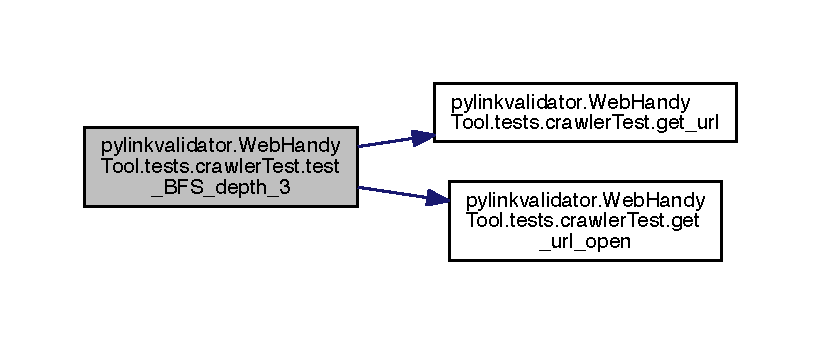
\includegraphics[width=350pt]{classpylinkvalidator_1_1_web_handy_tool_1_1tests_1_1crawler_test_a92c82295f6e332a249a11868f5999218_cgraph}
\end{center}
\end{figure}


\index{pylinkvalidator\+::\+Web\+Handy\+Tool\+::tests\+::crawler\+Test@{pylinkvalidator\+::\+Web\+Handy\+Tool\+::tests\+::crawler\+Test}!test\+\_\+\+B\+F\+S\+\_\+depth\+\_\+4@{test\+\_\+\+B\+F\+S\+\_\+depth\+\_\+4}}
\index{test\+\_\+\+B\+F\+S\+\_\+depth\+\_\+4@{test\+\_\+\+B\+F\+S\+\_\+depth\+\_\+4}!pylinkvalidator\+::\+Web\+Handy\+Tool\+::tests\+::crawler\+Test@{pylinkvalidator\+::\+Web\+Handy\+Tool\+::tests\+::crawler\+Test}}
\subsubsection[{test\+\_\+\+B\+F\+S\+\_\+depth\+\_\+4(self)}]{\setlength{\rightskip}{0pt plus 5cm}def pylinkvalidator.\+Web\+Handy\+Tool.\+tests.\+crawler\+Test.\+test\+\_\+\+B\+F\+S\+\_\+depth\+\_\+4 (
\begin{DoxyParamCaption}
\item[{}]{self}
\end{DoxyParamCaption}
)}\hypertarget{classpylinkvalidator_1_1_web_handy_tool_1_1tests_1_1crawler_test_a433365f3474025469ab42635234cbef0}{}\label{classpylinkvalidator_1_1_web_handy_tool_1_1tests_1_1crawler_test_a433365f3474025469ab42635234cbef0}


Here is the call graph for this function\+:
\nopagebreak
\begin{figure}[H]
\begin{center}
\leavevmode
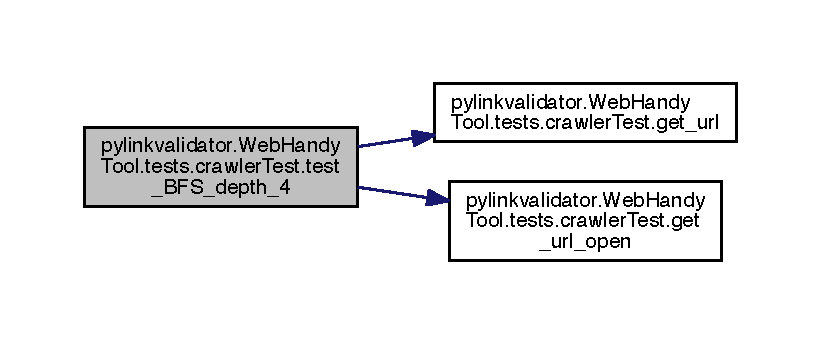
\includegraphics[width=350pt]{classpylinkvalidator_1_1_web_handy_tool_1_1tests_1_1crawler_test_a433365f3474025469ab42635234cbef0_cgraph}
\end{center}
\end{figure}


\index{pylinkvalidator\+::\+Web\+Handy\+Tool\+::tests\+::crawler\+Test@{pylinkvalidator\+::\+Web\+Handy\+Tool\+::tests\+::crawler\+Test}!test\+\_\+\+B\+F\+S\+\_\+depth\+\_\+5@{test\+\_\+\+B\+F\+S\+\_\+depth\+\_\+5}}
\index{test\+\_\+\+B\+F\+S\+\_\+depth\+\_\+5@{test\+\_\+\+B\+F\+S\+\_\+depth\+\_\+5}!pylinkvalidator\+::\+Web\+Handy\+Tool\+::tests\+::crawler\+Test@{pylinkvalidator\+::\+Web\+Handy\+Tool\+::tests\+::crawler\+Test}}
\subsubsection[{test\+\_\+\+B\+F\+S\+\_\+depth\+\_\+5(self)}]{\setlength{\rightskip}{0pt plus 5cm}def pylinkvalidator.\+Web\+Handy\+Tool.\+tests.\+crawler\+Test.\+test\+\_\+\+B\+F\+S\+\_\+depth\+\_\+5 (
\begin{DoxyParamCaption}
\item[{}]{self}
\end{DoxyParamCaption}
)}\hypertarget{classpylinkvalidator_1_1_web_handy_tool_1_1tests_1_1crawler_test_a96a6738fbd35cf6397c417d262dd30f0}{}\label{classpylinkvalidator_1_1_web_handy_tool_1_1tests_1_1crawler_test_a96a6738fbd35cf6397c417d262dd30f0}


Here is the call graph for this function\+:
\nopagebreak
\begin{figure}[H]
\begin{center}
\leavevmode
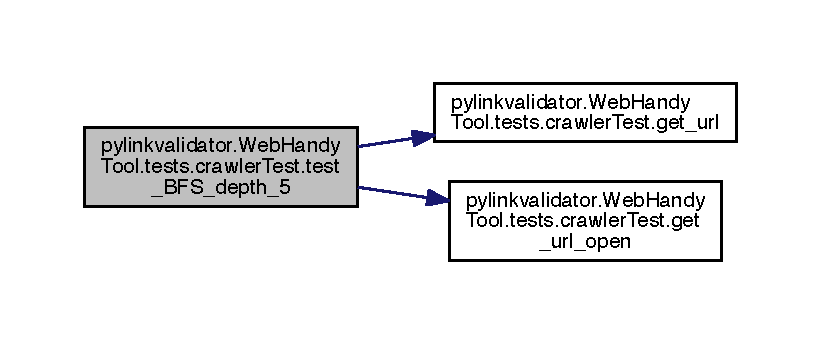
\includegraphics[width=350pt]{classpylinkvalidator_1_1_web_handy_tool_1_1tests_1_1crawler_test_a96a6738fbd35cf6397c417d262dd30f0_cgraph}
\end{center}
\end{figure}


\index{pylinkvalidator\+::\+Web\+Handy\+Tool\+::tests\+::crawler\+Test@{pylinkvalidator\+::\+Web\+Handy\+Tool\+::tests\+::crawler\+Test}!test\+\_\+download@{test\+\_\+download}}
\index{test\+\_\+download@{test\+\_\+download}!pylinkvalidator\+::\+Web\+Handy\+Tool\+::tests\+::crawler\+Test@{pylinkvalidator\+::\+Web\+Handy\+Tool\+::tests\+::crawler\+Test}}
\subsubsection[{test\+\_\+download(self)}]{\setlength{\rightskip}{0pt plus 5cm}def pylinkvalidator.\+Web\+Handy\+Tool.\+tests.\+crawler\+Test.\+test\+\_\+download (
\begin{DoxyParamCaption}
\item[{}]{self}
\end{DoxyParamCaption}
)}\hypertarget{classpylinkvalidator_1_1_web_handy_tool_1_1tests_1_1crawler_test_a4f86d42852e498de1c0d70b11c8950a1}{}\label{classpylinkvalidator_1_1_web_handy_tool_1_1tests_1_1crawler_test_a4f86d42852e498de1c0d70b11c8950a1}


Here is the call graph for this function\+:
\nopagebreak
\begin{figure}[H]
\begin{center}
\leavevmode
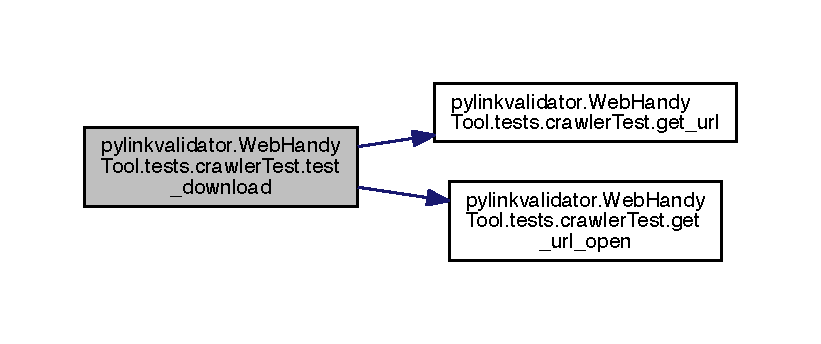
\includegraphics[width=350pt]{classpylinkvalidator_1_1_web_handy_tool_1_1tests_1_1crawler_test_a4f86d42852e498de1c0d70b11c8950a1_cgraph}
\end{center}
\end{figure}


\index{pylinkvalidator\+::\+Web\+Handy\+Tool\+::tests\+::crawler\+Test@{pylinkvalidator\+::\+Web\+Handy\+Tool\+::tests\+::crawler\+Test}!test\+\_\+link\+\_\+grabber@{test\+\_\+link\+\_\+grabber}}
\index{test\+\_\+link\+\_\+grabber@{test\+\_\+link\+\_\+grabber}!pylinkvalidator\+::\+Web\+Handy\+Tool\+::tests\+::crawler\+Test@{pylinkvalidator\+::\+Web\+Handy\+Tool\+::tests\+::crawler\+Test}}
\subsubsection[{test\+\_\+link\+\_\+grabber(self)}]{\setlength{\rightskip}{0pt plus 5cm}def pylinkvalidator.\+Web\+Handy\+Tool.\+tests.\+crawler\+Test.\+test\+\_\+link\+\_\+grabber (
\begin{DoxyParamCaption}
\item[{}]{self}
\end{DoxyParamCaption}
)}\hypertarget{classpylinkvalidator_1_1_web_handy_tool_1_1tests_1_1crawler_test_ac00856c89d2d4130ffe0ca385df3f679}{}\label{classpylinkvalidator_1_1_web_handy_tool_1_1tests_1_1crawler_test_ac00856c89d2d4130ffe0ca385df3f679}


Here is the call graph for this function\+:
\nopagebreak
\begin{figure}[H]
\begin{center}
\leavevmode
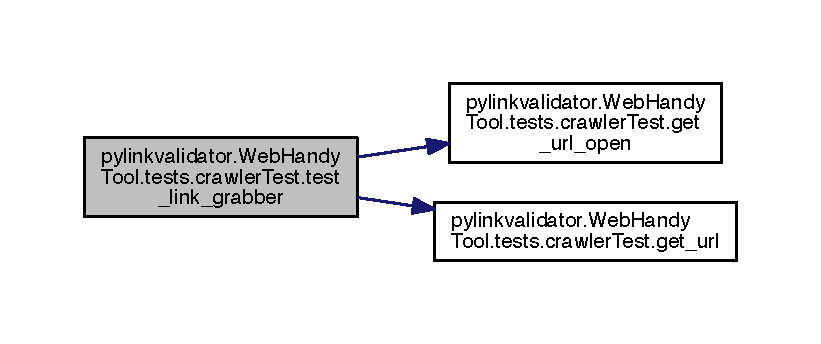
\includegraphics[width=350pt]{classpylinkvalidator_1_1_web_handy_tool_1_1tests_1_1crawler_test_ac00856c89d2d4130ffe0ca385df3f679_cgraph}
\end{center}
\end{figure}




The documentation for this class was generated from the following file\+:\begin{DoxyCompactItemize}
\item 
Web\+Handy\+Tool/\hyperlink{tests_8py}{tests.\+py}\end{DoxyCompactItemize}

\hypertarget{classpylinkvalidator_1_1_web_handy_tool_1_1download_1_1download}{}\section{pylinkvalidator.\+Web\+Handy\+Tool.\+download.\+download Class Reference}
\label{classpylinkvalidator_1_1_web_handy_tool_1_1download_1_1download}\index{pylinkvalidator.\+Web\+Handy\+Tool.\+download.\+download@{pylinkvalidator.\+Web\+Handy\+Tool.\+download.\+download}}


Inheritance diagram for pylinkvalidator.\+Web\+Handy\+Tool.\+download.\+download\+:
\nopagebreak
\begin{figure}[H]
\begin{center}
\leavevmode
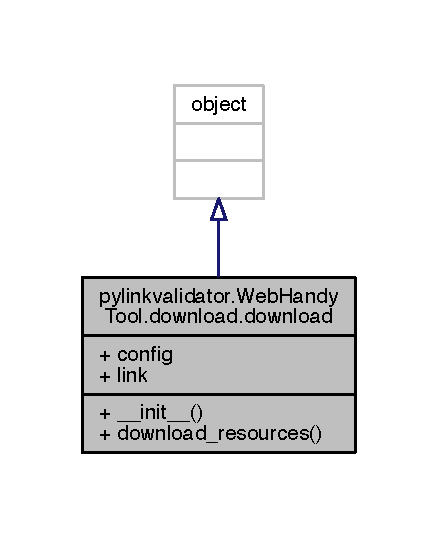
\includegraphics[width=210pt]{classpylinkvalidator_1_1_web_handy_tool_1_1download_1_1download__inherit__graph}
\end{center}
\end{figure}


Collaboration diagram for pylinkvalidator.\+Web\+Handy\+Tool.\+download.\+download\+:
\nopagebreak
\begin{figure}[H]
\begin{center}
\leavevmode
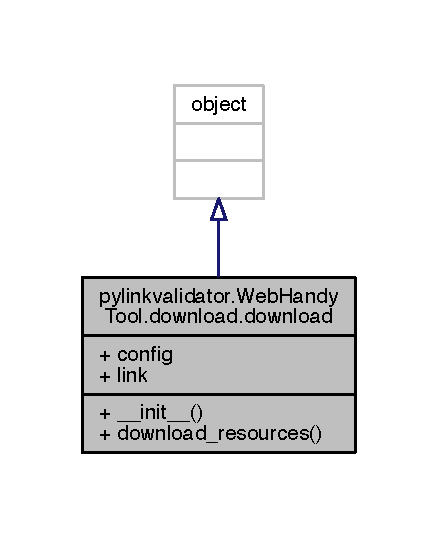
\includegraphics[width=210pt]{classpylinkvalidator_1_1_web_handy_tool_1_1download_1_1download__coll__graph}
\end{center}
\end{figure}
\subsection*{Public Member Functions}
\begin{DoxyCompactItemize}
\item 
def \hyperlink{classpylinkvalidator_1_1_web_handy_tool_1_1download_1_1download_ae62fcb67ed597f005b4e56a5e362eeec}{\+\_\+\+\_\+init\+\_\+\+\_\+} (self)
\item 
def \hyperlink{classpylinkvalidator_1_1_web_handy_tool_1_1download_1_1download_abaf45f1689c16761058cdc9fd5642083}{download\+\_\+resources} (self, \hyperlink{classpylinkvalidator_1_1_web_handy_tool_1_1download_1_1download_ae797f56e959b627f4146563aaf63353a}{link}, file\+\_\+type=None)
\end{DoxyCompactItemize}
\subsection*{Public Attributes}
\begin{DoxyCompactItemize}
\item 
\hyperlink{classpylinkvalidator_1_1_web_handy_tool_1_1download_1_1download_a11fcd57c43233322454323c791dec35e}{config}
\item 
\hyperlink{classpylinkvalidator_1_1_web_handy_tool_1_1download_1_1download_ae797f56e959b627f4146563aaf63353a}{link}
\end{DoxyCompactItemize}


\subsection{Constructor \& Destructor Documentation}
\index{pylinkvalidator\+::\+Web\+Handy\+Tool\+::download\+::download@{pylinkvalidator\+::\+Web\+Handy\+Tool\+::download\+::download}!\+\_\+\+\_\+init\+\_\+\+\_\+@{\+\_\+\+\_\+init\+\_\+\+\_\+}}
\index{\+\_\+\+\_\+init\+\_\+\+\_\+@{\+\_\+\+\_\+init\+\_\+\+\_\+}!pylinkvalidator\+::\+Web\+Handy\+Tool\+::download\+::download@{pylinkvalidator\+::\+Web\+Handy\+Tool\+::download\+::download}}
\subsubsection[{\+\_\+\+\_\+init\+\_\+\+\_\+(self)}]{\setlength{\rightskip}{0pt plus 5cm}def pylinkvalidator.\+Web\+Handy\+Tool.\+download.\+download.\+\_\+\+\_\+init\+\_\+\+\_\+ (
\begin{DoxyParamCaption}
\item[{}]{self}
\end{DoxyParamCaption}
)}\hypertarget{classpylinkvalidator_1_1_web_handy_tool_1_1download_1_1download_ae62fcb67ed597f005b4e56a5e362eeec}{}\label{classpylinkvalidator_1_1_web_handy_tool_1_1download_1_1download_ae62fcb67ed597f005b4e56a5e362eeec}


\subsection{Member Function Documentation}
\index{pylinkvalidator\+::\+Web\+Handy\+Tool\+::download\+::download@{pylinkvalidator\+::\+Web\+Handy\+Tool\+::download\+::download}!download\+\_\+resources@{download\+\_\+resources}}
\index{download\+\_\+resources@{download\+\_\+resources}!pylinkvalidator\+::\+Web\+Handy\+Tool\+::download\+::download@{pylinkvalidator\+::\+Web\+Handy\+Tool\+::download\+::download}}
\subsubsection[{download\+\_\+resources(self, link, file\+\_\+type=\+None)}]{\setlength{\rightskip}{0pt plus 5cm}def pylinkvalidator.\+Web\+Handy\+Tool.\+download.\+download.\+download\+\_\+resources (
\begin{DoxyParamCaption}
\item[{}]{self, }
\item[{}]{link, }
\item[{}]{file\+\_\+type = {\ttfamily None}}
\end{DoxyParamCaption}
)}\hypertarget{classpylinkvalidator_1_1_web_handy_tool_1_1download_1_1download_abaf45f1689c16761058cdc9fd5642083}{}\label{classpylinkvalidator_1_1_web_handy_tool_1_1download_1_1download_abaf45f1689c16761058cdc9fd5642083}
\begin{DoxyVerb}Writes all resources matching the given file type from the page link to the file specified by destination.

:param link:
:param options:
:param file_type:
:return:
\end{DoxyVerb}
 

\subsection{Member Data Documentation}
\index{pylinkvalidator\+::\+Web\+Handy\+Tool\+::download\+::download@{pylinkvalidator\+::\+Web\+Handy\+Tool\+::download\+::download}!config@{config}}
\index{config@{config}!pylinkvalidator\+::\+Web\+Handy\+Tool\+::download\+::download@{pylinkvalidator\+::\+Web\+Handy\+Tool\+::download\+::download}}
\subsubsection[{config}]{\setlength{\rightskip}{0pt plus 5cm}pylinkvalidator.\+Web\+Handy\+Tool.\+download.\+download.\+config}\hypertarget{classpylinkvalidator_1_1_web_handy_tool_1_1download_1_1download_a11fcd57c43233322454323c791dec35e}{}\label{classpylinkvalidator_1_1_web_handy_tool_1_1download_1_1download_a11fcd57c43233322454323c791dec35e}
\index{pylinkvalidator\+::\+Web\+Handy\+Tool\+::download\+::download@{pylinkvalidator\+::\+Web\+Handy\+Tool\+::download\+::download}!link@{link}}
\index{link@{link}!pylinkvalidator\+::\+Web\+Handy\+Tool\+::download\+::download@{pylinkvalidator\+::\+Web\+Handy\+Tool\+::download\+::download}}
\subsubsection[{link}]{\setlength{\rightskip}{0pt plus 5cm}pylinkvalidator.\+Web\+Handy\+Tool.\+download.\+download.\+link}\hypertarget{classpylinkvalidator_1_1_web_handy_tool_1_1download_1_1download_ae797f56e959b627f4146563aaf63353a}{}\label{classpylinkvalidator_1_1_web_handy_tool_1_1download_1_1download_ae797f56e959b627f4146563aaf63353a}


The documentation for this class was generated from the following file\+:\begin{DoxyCompactItemize}
\item 
Web\+Handy\+Tool/\hyperlink{download_8py}{download.\+py}\end{DoxyCompactItemize}

\hypertarget{classpylinkvalidator_1_1_web_handy_tool_1_1errors_1_1errors}{}\section{pylinkvalidator.\+Web\+Handy\+Tool.\+errors.\+errors Class Reference}
\label{classpylinkvalidator_1_1_web_handy_tool_1_1errors_1_1errors}\index{pylinkvalidator.\+Web\+Handy\+Tool.\+errors.\+errors@{pylinkvalidator.\+Web\+Handy\+Tool.\+errors.\+errors}}


Inheritance diagram for pylinkvalidator.\+Web\+Handy\+Tool.\+errors.\+errors\+:
\nopagebreak
\begin{figure}[H]
\begin{center}
\leavevmode
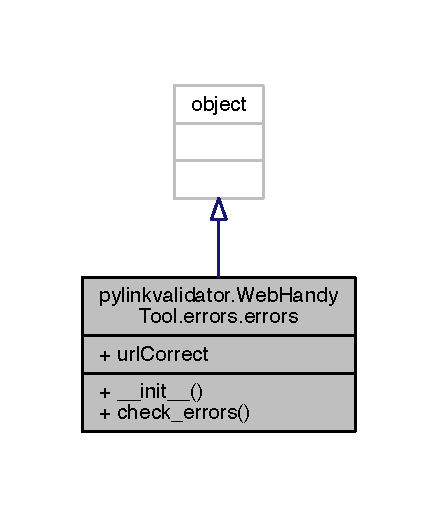
\includegraphics[width=210pt]{classpylinkvalidator_1_1_web_handy_tool_1_1errors_1_1errors__inherit__graph}
\end{center}
\end{figure}


Collaboration diagram for pylinkvalidator.\+Web\+Handy\+Tool.\+errors.\+errors\+:
\nopagebreak
\begin{figure}[H]
\begin{center}
\leavevmode
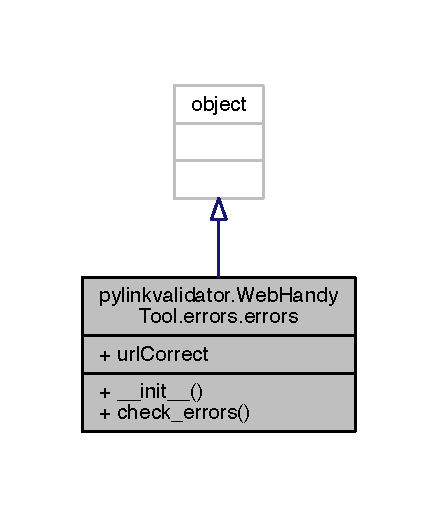
\includegraphics[width=210pt]{classpylinkvalidator_1_1_web_handy_tool_1_1errors_1_1errors__coll__graph}
\end{center}
\end{figure}
\subsection*{Public Member Functions}
\begin{DoxyCompactItemize}
\item 
def \hyperlink{classpylinkvalidator_1_1_web_handy_tool_1_1errors_1_1errors_a897c66f55e075d1bb5df00ad5dd966ab}{\+\_\+\+\_\+init\+\_\+\+\_\+} (self)
\item 
def \hyperlink{classpylinkvalidator_1_1_web_handy_tool_1_1errors_1_1errors_a560745957eb76bc1b2ea4acb29a42798}{check\+\_\+errors} (self, link, list\+\_\+of\+\_\+links=None)
\end{DoxyCompactItemize}
\subsection*{Public Attributes}
\begin{DoxyCompactItemize}
\item 
\hyperlink{classpylinkvalidator_1_1_web_handy_tool_1_1errors_1_1errors_a25aadeefbd1492f5efd8690cb1deecb5}{url\+Correct}
\end{DoxyCompactItemize}


\subsection{Constructor \& Destructor Documentation}
\index{pylinkvalidator\+::\+Web\+Handy\+Tool\+::errors\+::errors@{pylinkvalidator\+::\+Web\+Handy\+Tool\+::errors\+::errors}!\+\_\+\+\_\+init\+\_\+\+\_\+@{\+\_\+\+\_\+init\+\_\+\+\_\+}}
\index{\+\_\+\+\_\+init\+\_\+\+\_\+@{\+\_\+\+\_\+init\+\_\+\+\_\+}!pylinkvalidator\+::\+Web\+Handy\+Tool\+::errors\+::errors@{pylinkvalidator\+::\+Web\+Handy\+Tool\+::errors\+::errors}}
\subsubsection[{\+\_\+\+\_\+init\+\_\+\+\_\+(self)}]{\setlength{\rightskip}{0pt plus 5cm}def pylinkvalidator.\+Web\+Handy\+Tool.\+errors.\+errors.\+\_\+\+\_\+init\+\_\+\+\_\+ (
\begin{DoxyParamCaption}
\item[{}]{self}
\end{DoxyParamCaption}
)}\hypertarget{classpylinkvalidator_1_1_web_handy_tool_1_1errors_1_1errors_a897c66f55e075d1bb5df00ad5dd966ab}{}\label{classpylinkvalidator_1_1_web_handy_tool_1_1errors_1_1errors_a897c66f55e075d1bb5df00ad5dd966ab}


\subsection{Member Function Documentation}
\index{pylinkvalidator\+::\+Web\+Handy\+Tool\+::errors\+::errors@{pylinkvalidator\+::\+Web\+Handy\+Tool\+::errors\+::errors}!check\+\_\+errors@{check\+\_\+errors}}
\index{check\+\_\+errors@{check\+\_\+errors}!pylinkvalidator\+::\+Web\+Handy\+Tool\+::errors\+::errors@{pylinkvalidator\+::\+Web\+Handy\+Tool\+::errors\+::errors}}
\subsubsection[{check\+\_\+errors(self, link, list\+\_\+of\+\_\+links=\+None)}]{\setlength{\rightskip}{0pt plus 5cm}def pylinkvalidator.\+Web\+Handy\+Tool.\+errors.\+errors.\+check\+\_\+errors (
\begin{DoxyParamCaption}
\item[{}]{self, }
\item[{}]{link, }
\item[{}]{list\+\_\+of\+\_\+links = {\ttfamily None}}
\end{DoxyParamCaption}
)}\hypertarget{classpylinkvalidator_1_1_web_handy_tool_1_1errors_1_1errors_a560745957eb76bc1b2ea4acb29a42798}{}\label{classpylinkvalidator_1_1_web_handy_tool_1_1errors_1_1errors_a560745957eb76bc1b2ea4acb29a42798}
\begin{DoxyVerb}Checks the all the links and reports the error message associated with
all the links inputted

:param link:
:param list_of_links:
:return List of Errors:
\end{DoxyVerb}
 

\subsection{Member Data Documentation}
\index{pylinkvalidator\+::\+Web\+Handy\+Tool\+::errors\+::errors@{pylinkvalidator\+::\+Web\+Handy\+Tool\+::errors\+::errors}!url\+Correct@{url\+Correct}}
\index{url\+Correct@{url\+Correct}!pylinkvalidator\+::\+Web\+Handy\+Tool\+::errors\+::errors@{pylinkvalidator\+::\+Web\+Handy\+Tool\+::errors\+::errors}}
\subsubsection[{url\+Correct}]{\setlength{\rightskip}{0pt plus 5cm}pylinkvalidator.\+Web\+Handy\+Tool.\+errors.\+errors.\+url\+Correct}\hypertarget{classpylinkvalidator_1_1_web_handy_tool_1_1errors_1_1errors_a25aadeefbd1492f5efd8690cb1deecb5}{}\label{classpylinkvalidator_1_1_web_handy_tool_1_1errors_1_1errors_a25aadeefbd1492f5efd8690cb1deecb5}


The documentation for this class was generated from the following file\+:\begin{DoxyCompactItemize}
\item 
Web\+Handy\+Tool/\hyperlink{errors_8py}{errors.\+py}\end{DoxyCompactItemize}

\hypertarget{classpylinkvalidator_1_1_p_o_c_01_code_1_1_web___crawler_1_1_h_t_m_l__corrector__help}{}\section{pylinkvalidator.\+P\+OC Code.\+Web\+\_\+\+Crawler.\+H\+T\+M\+L\+\_\+corrector\+\_\+help Class Reference}
\label{classpylinkvalidator_1_1_p_o_c_01_code_1_1_web___crawler_1_1_h_t_m_l__corrector__help}\index{pylinkvalidator.\+P\+O\+C Code.\+Web\+\_\+\+Crawler.\+H\+T\+M\+L\+\_\+corrector\+\_\+help@{pylinkvalidator.\+P\+O\+C Code.\+Web\+\_\+\+Crawler.\+H\+T\+M\+L\+\_\+corrector\+\_\+help}}


Inheritance diagram for pylinkvalidator.\+P\+OC Code.\+Web\+\_\+\+Crawler.\+H\+T\+M\+L\+\_\+corrector\+\_\+help\+:
\nopagebreak
\begin{figure}[H]
\begin{center}
\leavevmode
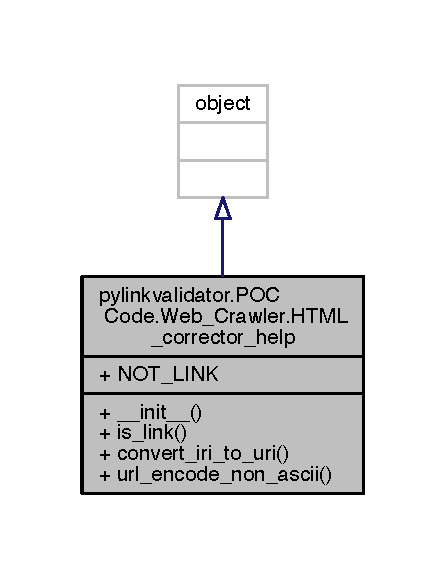
\includegraphics[width=214pt]{classpylinkvalidator_1_1_p_o_c_01_code_1_1_web___crawler_1_1_h_t_m_l__corrector__help__inherit__graph}
\end{center}
\end{figure}


Collaboration diagram for pylinkvalidator.\+P\+OC Code.\+Web\+\_\+\+Crawler.\+H\+T\+M\+L\+\_\+corrector\+\_\+help\+:
\nopagebreak
\begin{figure}[H]
\begin{center}
\leavevmode
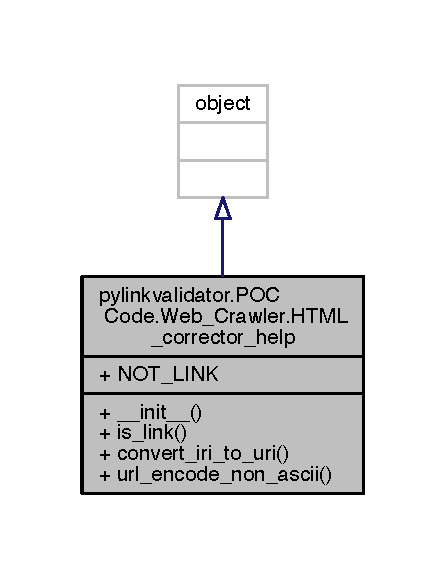
\includegraphics[width=214pt]{classpylinkvalidator_1_1_p_o_c_01_code_1_1_web___crawler_1_1_h_t_m_l__corrector__help__coll__graph}
\end{center}
\end{figure}
\subsection*{Public Member Functions}
\begin{DoxyCompactItemize}
\item 
def \hyperlink{classpylinkvalidator_1_1_p_o_c_01_code_1_1_web___crawler_1_1_h_t_m_l__corrector__help_a74a8cbe051183c34bc6326175808b44a}{\+\_\+\+\_\+init\+\_\+\+\_\+} (self)
\item 
def \hyperlink{classpylinkvalidator_1_1_p_o_c_01_code_1_1_web___crawler_1_1_h_t_m_l__corrector__help_ac5786be0512ad6da9959426d38890919}{is\+\_\+link} (self, url)
\item 
def \hyperlink{classpylinkvalidator_1_1_p_o_c_01_code_1_1_web___crawler_1_1_h_t_m_l__corrector__help_af6b498d8b0c15bd9e103906e099e48f5}{convert\+\_\+iri\+\_\+to\+\_\+uri} (self, url\+\_\+split)
\item 
def \hyperlink{classpylinkvalidator_1_1_p_o_c_01_code_1_1_web___crawler_1_1_h_t_m_l__corrector__help_ac8fb606d19d641436906401f41a1ca2f}{url\+\_\+encode\+\_\+non\+\_\+ascii} (self, url\+\_\+part)
\end{DoxyCompactItemize}
\subsection*{Public Attributes}
\begin{DoxyCompactItemize}
\item 
\hyperlink{classpylinkvalidator_1_1_p_o_c_01_code_1_1_web___crawler_1_1_h_t_m_l__corrector__help_a862769bf382fae597f7be261e69ebf0a}{N\+O\+T\+\_\+\+L\+I\+NK}
\end{DoxyCompactItemize}


\subsection{Detailed Description}
\begin{DoxyVerb}Library of helper functions that are used by HTML corrector to
fix url links.
\end{DoxyVerb}
 

\subsection{Constructor \& Destructor Documentation}
\index{pylinkvalidator\+::\+P\+O\+C Code\+::\+Web\+\_\+\+Crawler\+::\+H\+T\+M\+L\+\_\+corrector\+\_\+help@{pylinkvalidator\+::\+P\+O\+C Code\+::\+Web\+\_\+\+Crawler\+::\+H\+T\+M\+L\+\_\+corrector\+\_\+help}!\+\_\+\+\_\+init\+\_\+\+\_\+@{\+\_\+\+\_\+init\+\_\+\+\_\+}}
\index{\+\_\+\+\_\+init\+\_\+\+\_\+@{\+\_\+\+\_\+init\+\_\+\+\_\+}!pylinkvalidator\+::\+P\+O\+C Code\+::\+Web\+\_\+\+Crawler\+::\+H\+T\+M\+L\+\_\+corrector\+\_\+help@{pylinkvalidator\+::\+P\+O\+C Code\+::\+Web\+\_\+\+Crawler\+::\+H\+T\+M\+L\+\_\+corrector\+\_\+help}}
\subsubsection[{\+\_\+\+\_\+init\+\_\+\+\_\+(self)}]{\setlength{\rightskip}{0pt plus 5cm}def pylinkvalidator.\+P\+OC Code.\+Web\+\_\+\+Crawler.\+H\+T\+M\+L\+\_\+corrector\+\_\+help.\+\_\+\+\_\+init\+\_\+\+\_\+ (
\begin{DoxyParamCaption}
\item[{}]{self}
\end{DoxyParamCaption}
)}\hypertarget{classpylinkvalidator_1_1_p_o_c_01_code_1_1_web___crawler_1_1_h_t_m_l__corrector__help_a74a8cbe051183c34bc6326175808b44a}{}\label{classpylinkvalidator_1_1_p_o_c_01_code_1_1_web___crawler_1_1_h_t_m_l__corrector__help_a74a8cbe051183c34bc6326175808b44a}


\subsection{Member Function Documentation}
\index{pylinkvalidator\+::\+P\+O\+C Code\+::\+Web\+\_\+\+Crawler\+::\+H\+T\+M\+L\+\_\+corrector\+\_\+help@{pylinkvalidator\+::\+P\+O\+C Code\+::\+Web\+\_\+\+Crawler\+::\+H\+T\+M\+L\+\_\+corrector\+\_\+help}!convert\+\_\+iri\+\_\+to\+\_\+uri@{convert\+\_\+iri\+\_\+to\+\_\+uri}}
\index{convert\+\_\+iri\+\_\+to\+\_\+uri@{convert\+\_\+iri\+\_\+to\+\_\+uri}!pylinkvalidator\+::\+P\+O\+C Code\+::\+Web\+\_\+\+Crawler\+::\+H\+T\+M\+L\+\_\+corrector\+\_\+help@{pylinkvalidator\+::\+P\+O\+C Code\+::\+Web\+\_\+\+Crawler\+::\+H\+T\+M\+L\+\_\+corrector\+\_\+help}}
\subsubsection[{convert\+\_\+iri\+\_\+to\+\_\+uri(self, url\+\_\+split)}]{\setlength{\rightskip}{0pt plus 5cm}def pylinkvalidator.\+P\+OC Code.\+Web\+\_\+\+Crawler.\+H\+T\+M\+L\+\_\+corrector\+\_\+help.\+convert\+\_\+iri\+\_\+to\+\_\+uri (
\begin{DoxyParamCaption}
\item[{}]{self, }
\item[{}]{url\+\_\+split}
\end{DoxyParamCaption}
)}\hypertarget{classpylinkvalidator_1_1_p_o_c_01_code_1_1_web___crawler_1_1_h_t_m_l__corrector__help_af6b498d8b0c15bd9e103906e099e48f5}{}\label{classpylinkvalidator_1_1_p_o_c_01_code_1_1_web___crawler_1_1_h_t_m_l__corrector__help_af6b498d8b0c15bd9e103906e099e48f5}
\begin{DoxyVerb}Attempts to convert potential IRI to URI.

IRI may contain non-ascii characters.
:param url_split:
:return:
\end{DoxyVerb}
 

Here is the call graph for this function\+:
\nopagebreak
\begin{figure}[H]
\begin{center}
\leavevmode
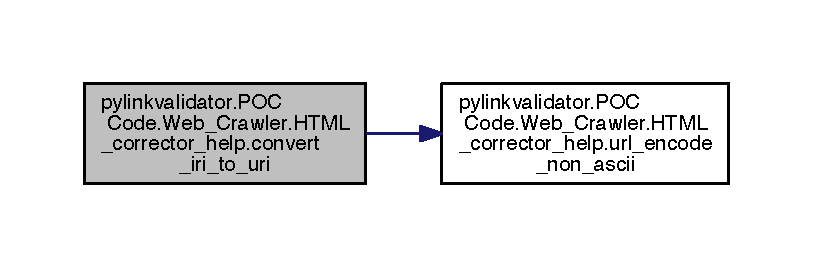
\includegraphics[width=350pt]{classpylinkvalidator_1_1_p_o_c_01_code_1_1_web___crawler_1_1_h_t_m_l__corrector__help_af6b498d8b0c15bd9e103906e099e48f5_cgraph}
\end{center}
\end{figure}


\index{pylinkvalidator\+::\+P\+O\+C Code\+::\+Web\+\_\+\+Crawler\+::\+H\+T\+M\+L\+\_\+corrector\+\_\+help@{pylinkvalidator\+::\+P\+O\+C Code\+::\+Web\+\_\+\+Crawler\+::\+H\+T\+M\+L\+\_\+corrector\+\_\+help}!is\+\_\+link@{is\+\_\+link}}
\index{is\+\_\+link@{is\+\_\+link}!pylinkvalidator\+::\+P\+O\+C Code\+::\+Web\+\_\+\+Crawler\+::\+H\+T\+M\+L\+\_\+corrector\+\_\+help@{pylinkvalidator\+::\+P\+O\+C Code\+::\+Web\+\_\+\+Crawler\+::\+H\+T\+M\+L\+\_\+corrector\+\_\+help}}
\subsubsection[{is\+\_\+link(self, url)}]{\setlength{\rightskip}{0pt plus 5cm}def pylinkvalidator.\+P\+OC Code.\+Web\+\_\+\+Crawler.\+H\+T\+M\+L\+\_\+corrector\+\_\+help.\+is\+\_\+link (
\begin{DoxyParamCaption}
\item[{}]{self, }
\item[{}]{url}
\end{DoxyParamCaption}
)}\hypertarget{classpylinkvalidator_1_1_p_o_c_01_code_1_1_web___crawler_1_1_h_t_m_l__corrector__help_ac5786be0512ad6da9959426d38890919}{}\label{classpylinkvalidator_1_1_p_o_c_01_code_1_1_web___crawler_1_1_h_t_m_l__corrector__help_ac5786be0512ad6da9959426d38890919}
\begin{DoxyVerb}Return True if the url is not base 64 data or a local ref (#)

:param url:
:return Boolean either True or False:
\end{DoxyVerb}
 \index{pylinkvalidator\+::\+P\+O\+C Code\+::\+Web\+\_\+\+Crawler\+::\+H\+T\+M\+L\+\_\+corrector\+\_\+help@{pylinkvalidator\+::\+P\+O\+C Code\+::\+Web\+\_\+\+Crawler\+::\+H\+T\+M\+L\+\_\+corrector\+\_\+help}!url\+\_\+encode\+\_\+non\+\_\+ascii@{url\+\_\+encode\+\_\+non\+\_\+ascii}}
\index{url\+\_\+encode\+\_\+non\+\_\+ascii@{url\+\_\+encode\+\_\+non\+\_\+ascii}!pylinkvalidator\+::\+P\+O\+C Code\+::\+Web\+\_\+\+Crawler\+::\+H\+T\+M\+L\+\_\+corrector\+\_\+help@{pylinkvalidator\+::\+P\+O\+C Code\+::\+Web\+\_\+\+Crawler\+::\+H\+T\+M\+L\+\_\+corrector\+\_\+help}}
\subsubsection[{url\+\_\+encode\+\_\+non\+\_\+ascii(self, url\+\_\+part)}]{\setlength{\rightskip}{0pt plus 5cm}def pylinkvalidator.\+P\+OC Code.\+Web\+\_\+\+Crawler.\+H\+T\+M\+L\+\_\+corrector\+\_\+help.\+url\+\_\+encode\+\_\+non\+\_\+ascii (
\begin{DoxyParamCaption}
\item[{}]{self, }
\item[{}]{url\+\_\+part}
\end{DoxyParamCaption}
)}\hypertarget{classpylinkvalidator_1_1_p_o_c_01_code_1_1_web___crawler_1_1_h_t_m_l__corrector__help_ac8fb606d19d641436906401f41a1ca2f}{}\label{classpylinkvalidator_1_1_p_o_c_01_code_1_1_web___crawler_1_1_h_t_m_l__corrector__help_ac8fb606d19d641436906401f41a1ca2f}
\begin{DoxyVerb}For each byte in url_part, if the byte is outside ascii range, quote the
byte. UTF characters that take two bytes will be correctly converted using
this technique.

We do not quote the whole url part because it might contain already quoted
characters, which would then be double-quoted.

The url part is converted from utf-8 and then to utf-8, which might not
always work if there is mixed or bad encoding.
:param url_part:
:return:
\end{DoxyVerb}
 

Here is the caller graph for this function\+:
\nopagebreak
\begin{figure}[H]
\begin{center}
\leavevmode
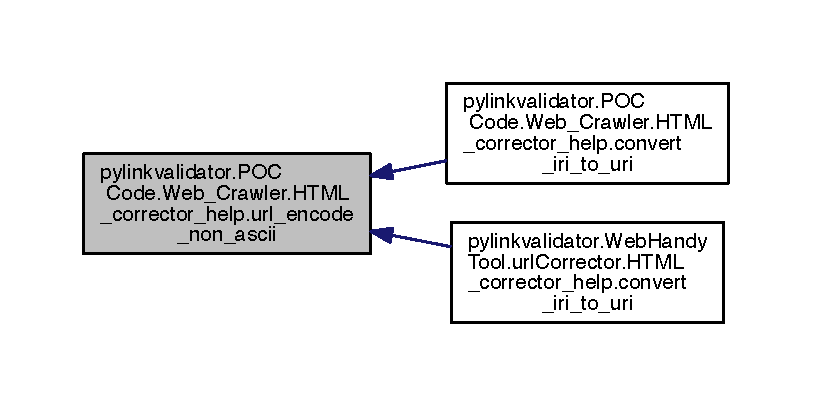
\includegraphics[width=350pt]{classpylinkvalidator_1_1_p_o_c_01_code_1_1_web___crawler_1_1_h_t_m_l__corrector__help_ac8fb606d19d641436906401f41a1ca2f_icgraph}
\end{center}
\end{figure}




\subsection{Member Data Documentation}
\index{pylinkvalidator\+::\+P\+O\+C Code\+::\+Web\+\_\+\+Crawler\+::\+H\+T\+M\+L\+\_\+corrector\+\_\+help@{pylinkvalidator\+::\+P\+O\+C Code\+::\+Web\+\_\+\+Crawler\+::\+H\+T\+M\+L\+\_\+corrector\+\_\+help}!N\+O\+T\+\_\+\+L\+I\+NK@{N\+O\+T\+\_\+\+L\+I\+NK}}
\index{N\+O\+T\+\_\+\+L\+I\+NK@{N\+O\+T\+\_\+\+L\+I\+NK}!pylinkvalidator\+::\+P\+O\+C Code\+::\+Web\+\_\+\+Crawler\+::\+H\+T\+M\+L\+\_\+corrector\+\_\+help@{pylinkvalidator\+::\+P\+O\+C Code\+::\+Web\+\_\+\+Crawler\+::\+H\+T\+M\+L\+\_\+corrector\+\_\+help}}
\subsubsection[{N\+O\+T\+\_\+\+L\+I\+NK}]{\setlength{\rightskip}{0pt plus 5cm}pylinkvalidator.\+P\+OC Code.\+Web\+\_\+\+Crawler.\+H\+T\+M\+L\+\_\+corrector\+\_\+help.\+N\+O\+T\+\_\+\+L\+I\+NK}\hypertarget{classpylinkvalidator_1_1_p_o_c_01_code_1_1_web___crawler_1_1_h_t_m_l__corrector__help_a862769bf382fae597f7be261e69ebf0a}{}\label{classpylinkvalidator_1_1_p_o_c_01_code_1_1_web___crawler_1_1_h_t_m_l__corrector__help_a862769bf382fae597f7be261e69ebf0a}


The documentation for this class was generated from the following file\+:\begin{DoxyCompactItemize}
\item 
P\+O\+C Code/\hyperlink{_p_o_c_01_code_2_web___crawler_8py}{Web\+\_\+\+Crawler.\+py}\end{DoxyCompactItemize}

\hypertarget{classpylinkvalidator_1_1_web_handy_tool_1_1url_corrector_1_1_h_t_m_l__corrector__help}{}\section{pylinkvalidator.\+Web\+Handy\+Tool.\+url\+Corrector.\+H\+T\+M\+L\+\_\+corrector\+\_\+help Class Reference}
\label{classpylinkvalidator_1_1_web_handy_tool_1_1url_corrector_1_1_h_t_m_l__corrector__help}\index{pylinkvalidator.\+Web\+Handy\+Tool.\+url\+Corrector.\+H\+T\+M\+L\+\_\+corrector\+\_\+help@{pylinkvalidator.\+Web\+Handy\+Tool.\+url\+Corrector.\+H\+T\+M\+L\+\_\+corrector\+\_\+help}}


Inheritance diagram for pylinkvalidator.\+Web\+Handy\+Tool.\+url\+Corrector.\+H\+T\+M\+L\+\_\+corrector\+\_\+help\+:
\nopagebreak
\begin{figure}[H]
\begin{center}
\leavevmode
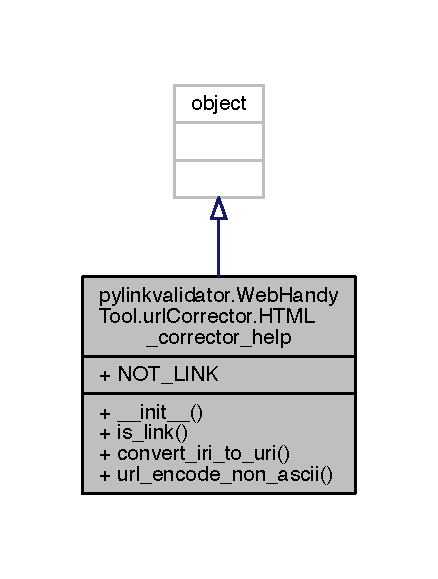
\includegraphics[width=210pt]{classpylinkvalidator_1_1_web_handy_tool_1_1url_corrector_1_1_h_t_m_l__corrector__help__inherit__graph}
\end{center}
\end{figure}


Collaboration diagram for pylinkvalidator.\+Web\+Handy\+Tool.\+url\+Corrector.\+H\+T\+M\+L\+\_\+corrector\+\_\+help\+:
\nopagebreak
\begin{figure}[H]
\begin{center}
\leavevmode
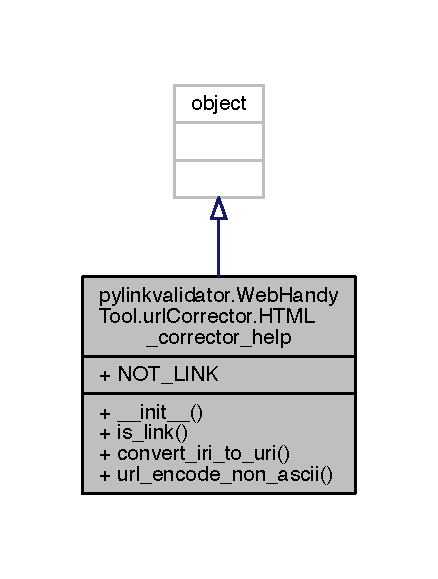
\includegraphics[width=210pt]{classpylinkvalidator_1_1_web_handy_tool_1_1url_corrector_1_1_h_t_m_l__corrector__help__coll__graph}
\end{center}
\end{figure}
\subsection*{Public Member Functions}
\begin{DoxyCompactItemize}
\item 
def \hyperlink{classpylinkvalidator_1_1_web_handy_tool_1_1url_corrector_1_1_h_t_m_l__corrector__help_ab6ebabc9defb9cba0d6dedb9254149b8}{\+\_\+\+\_\+init\+\_\+\+\_\+} (self)
\item 
def \hyperlink{classpylinkvalidator_1_1_web_handy_tool_1_1url_corrector_1_1_h_t_m_l__corrector__help_ae1494f4d37f13c5a1bc9a46e00b48bc5}{is\+\_\+link} (self, url)
\item 
def \hyperlink{classpylinkvalidator_1_1_web_handy_tool_1_1url_corrector_1_1_h_t_m_l__corrector__help_abc2880e66a8f0145fef8e1629f465d17}{convert\+\_\+iri\+\_\+to\+\_\+uri} (self, url\+\_\+split)
\item 
def \hyperlink{classpylinkvalidator_1_1_web_handy_tool_1_1url_corrector_1_1_h_t_m_l__corrector__help_a894ef6c5bc2150372a36b8c0abbca8d2}{url\+\_\+encode\+\_\+non\+\_\+ascii} (self, url\+\_\+part)
\end{DoxyCompactItemize}
\subsection*{Public Attributes}
\begin{DoxyCompactItemize}
\item 
\hyperlink{classpylinkvalidator_1_1_web_handy_tool_1_1url_corrector_1_1_h_t_m_l__corrector__help_a5b2cbd7348808b3fa573af6d89fd0bef}{N\+O\+T\+\_\+\+L\+I\+NK}
\end{DoxyCompactItemize}


\subsection{Detailed Description}
\begin{DoxyVerb}Library of helper functions that are used by HTML corrector to
fix url links.
\end{DoxyVerb}
 

\subsection{Constructor \& Destructor Documentation}
\index{pylinkvalidator\+::\+Web\+Handy\+Tool\+::url\+Corrector\+::\+H\+T\+M\+L\+\_\+corrector\+\_\+help@{pylinkvalidator\+::\+Web\+Handy\+Tool\+::url\+Corrector\+::\+H\+T\+M\+L\+\_\+corrector\+\_\+help}!\+\_\+\+\_\+init\+\_\+\+\_\+@{\+\_\+\+\_\+init\+\_\+\+\_\+}}
\index{\+\_\+\+\_\+init\+\_\+\+\_\+@{\+\_\+\+\_\+init\+\_\+\+\_\+}!pylinkvalidator\+::\+Web\+Handy\+Tool\+::url\+Corrector\+::\+H\+T\+M\+L\+\_\+corrector\+\_\+help@{pylinkvalidator\+::\+Web\+Handy\+Tool\+::url\+Corrector\+::\+H\+T\+M\+L\+\_\+corrector\+\_\+help}}
\subsubsection[{\+\_\+\+\_\+init\+\_\+\+\_\+(self)}]{\setlength{\rightskip}{0pt plus 5cm}def pylinkvalidator.\+Web\+Handy\+Tool.\+url\+Corrector.\+H\+T\+M\+L\+\_\+corrector\+\_\+help.\+\_\+\+\_\+init\+\_\+\+\_\+ (
\begin{DoxyParamCaption}
\item[{}]{self}
\end{DoxyParamCaption}
)}\hypertarget{classpylinkvalidator_1_1_web_handy_tool_1_1url_corrector_1_1_h_t_m_l__corrector__help_ab6ebabc9defb9cba0d6dedb9254149b8}{}\label{classpylinkvalidator_1_1_web_handy_tool_1_1url_corrector_1_1_h_t_m_l__corrector__help_ab6ebabc9defb9cba0d6dedb9254149b8}


\subsection{Member Function Documentation}
\index{pylinkvalidator\+::\+Web\+Handy\+Tool\+::url\+Corrector\+::\+H\+T\+M\+L\+\_\+corrector\+\_\+help@{pylinkvalidator\+::\+Web\+Handy\+Tool\+::url\+Corrector\+::\+H\+T\+M\+L\+\_\+corrector\+\_\+help}!convert\+\_\+iri\+\_\+to\+\_\+uri@{convert\+\_\+iri\+\_\+to\+\_\+uri}}
\index{convert\+\_\+iri\+\_\+to\+\_\+uri@{convert\+\_\+iri\+\_\+to\+\_\+uri}!pylinkvalidator\+::\+Web\+Handy\+Tool\+::url\+Corrector\+::\+H\+T\+M\+L\+\_\+corrector\+\_\+help@{pylinkvalidator\+::\+Web\+Handy\+Tool\+::url\+Corrector\+::\+H\+T\+M\+L\+\_\+corrector\+\_\+help}}
\subsubsection[{convert\+\_\+iri\+\_\+to\+\_\+uri(self, url\+\_\+split)}]{\setlength{\rightskip}{0pt plus 5cm}def pylinkvalidator.\+Web\+Handy\+Tool.\+url\+Corrector.\+H\+T\+M\+L\+\_\+corrector\+\_\+help.\+convert\+\_\+iri\+\_\+to\+\_\+uri (
\begin{DoxyParamCaption}
\item[{}]{self, }
\item[{}]{url\+\_\+split}
\end{DoxyParamCaption}
)}\hypertarget{classpylinkvalidator_1_1_web_handy_tool_1_1url_corrector_1_1_h_t_m_l__corrector__help_abc2880e66a8f0145fef8e1629f465d17}{}\label{classpylinkvalidator_1_1_web_handy_tool_1_1url_corrector_1_1_h_t_m_l__corrector__help_abc2880e66a8f0145fef8e1629f465d17}
\begin{DoxyVerb}Attempts to convert potential IRI to URI.

IRI may contain non-ascii characters.
:param url_split:
:return:
\end{DoxyVerb}
 

Here is the call graph for this function\+:
\nopagebreak
\begin{figure}[H]
\begin{center}
\leavevmode
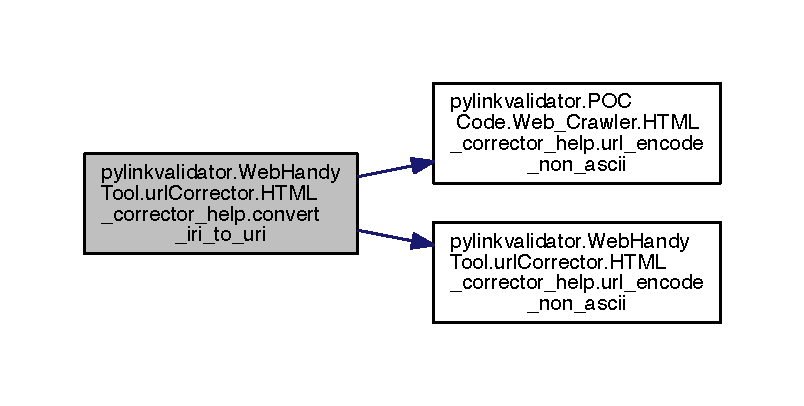
\includegraphics[width=350pt]{classpylinkvalidator_1_1_web_handy_tool_1_1url_corrector_1_1_h_t_m_l__corrector__help_abc2880e66a8f0145fef8e1629f465d17_cgraph}
\end{center}
\end{figure}


\index{pylinkvalidator\+::\+Web\+Handy\+Tool\+::url\+Corrector\+::\+H\+T\+M\+L\+\_\+corrector\+\_\+help@{pylinkvalidator\+::\+Web\+Handy\+Tool\+::url\+Corrector\+::\+H\+T\+M\+L\+\_\+corrector\+\_\+help}!is\+\_\+link@{is\+\_\+link}}
\index{is\+\_\+link@{is\+\_\+link}!pylinkvalidator\+::\+Web\+Handy\+Tool\+::url\+Corrector\+::\+H\+T\+M\+L\+\_\+corrector\+\_\+help@{pylinkvalidator\+::\+Web\+Handy\+Tool\+::url\+Corrector\+::\+H\+T\+M\+L\+\_\+corrector\+\_\+help}}
\subsubsection[{is\+\_\+link(self, url)}]{\setlength{\rightskip}{0pt plus 5cm}def pylinkvalidator.\+Web\+Handy\+Tool.\+url\+Corrector.\+H\+T\+M\+L\+\_\+corrector\+\_\+help.\+is\+\_\+link (
\begin{DoxyParamCaption}
\item[{}]{self, }
\item[{}]{url}
\end{DoxyParamCaption}
)}\hypertarget{classpylinkvalidator_1_1_web_handy_tool_1_1url_corrector_1_1_h_t_m_l__corrector__help_ae1494f4d37f13c5a1bc9a46e00b48bc5}{}\label{classpylinkvalidator_1_1_web_handy_tool_1_1url_corrector_1_1_h_t_m_l__corrector__help_ae1494f4d37f13c5a1bc9a46e00b48bc5}
\begin{DoxyVerb}Return True if the url is not base 64 data or a local ref (#)

:param url:
:return Boolean either True or False:
\end{DoxyVerb}
 \index{pylinkvalidator\+::\+Web\+Handy\+Tool\+::url\+Corrector\+::\+H\+T\+M\+L\+\_\+corrector\+\_\+help@{pylinkvalidator\+::\+Web\+Handy\+Tool\+::url\+Corrector\+::\+H\+T\+M\+L\+\_\+corrector\+\_\+help}!url\+\_\+encode\+\_\+non\+\_\+ascii@{url\+\_\+encode\+\_\+non\+\_\+ascii}}
\index{url\+\_\+encode\+\_\+non\+\_\+ascii@{url\+\_\+encode\+\_\+non\+\_\+ascii}!pylinkvalidator\+::\+Web\+Handy\+Tool\+::url\+Corrector\+::\+H\+T\+M\+L\+\_\+corrector\+\_\+help@{pylinkvalidator\+::\+Web\+Handy\+Tool\+::url\+Corrector\+::\+H\+T\+M\+L\+\_\+corrector\+\_\+help}}
\subsubsection[{url\+\_\+encode\+\_\+non\+\_\+ascii(self, url\+\_\+part)}]{\setlength{\rightskip}{0pt plus 5cm}def pylinkvalidator.\+Web\+Handy\+Tool.\+url\+Corrector.\+H\+T\+M\+L\+\_\+corrector\+\_\+help.\+url\+\_\+encode\+\_\+non\+\_\+ascii (
\begin{DoxyParamCaption}
\item[{}]{self, }
\item[{}]{url\+\_\+part}
\end{DoxyParamCaption}
)}\hypertarget{classpylinkvalidator_1_1_web_handy_tool_1_1url_corrector_1_1_h_t_m_l__corrector__help_a894ef6c5bc2150372a36b8c0abbca8d2}{}\label{classpylinkvalidator_1_1_web_handy_tool_1_1url_corrector_1_1_h_t_m_l__corrector__help_a894ef6c5bc2150372a36b8c0abbca8d2}
\begin{DoxyVerb}For each byte in url_part, if the byte is outside ascii range, quote the
byte. UTF characters that take two bytes will be correctly converted using
this technique.

We do not quote the whole url part because it might contain already quoted
characters, which would then be double-quoted.

The url part is converted from utf-8 and then to utf-8, which might not
always work if there is mixed or bad encoding.
:param url_part:
:return:
\end{DoxyVerb}
 

Here is the caller graph for this function\+:
\nopagebreak
\begin{figure}[H]
\begin{center}
\leavevmode
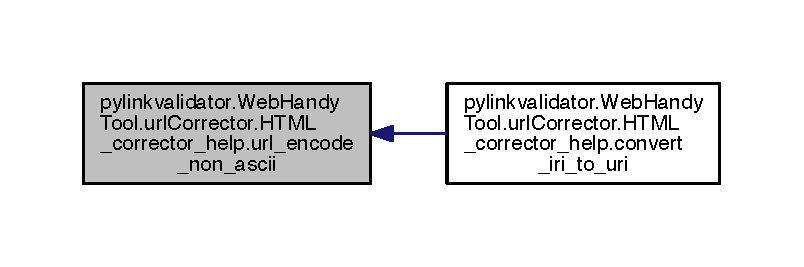
\includegraphics[width=350pt]{classpylinkvalidator_1_1_web_handy_tool_1_1url_corrector_1_1_h_t_m_l__corrector__help_a894ef6c5bc2150372a36b8c0abbca8d2_icgraph}
\end{center}
\end{figure}




\subsection{Member Data Documentation}
\index{pylinkvalidator\+::\+Web\+Handy\+Tool\+::url\+Corrector\+::\+H\+T\+M\+L\+\_\+corrector\+\_\+help@{pylinkvalidator\+::\+Web\+Handy\+Tool\+::url\+Corrector\+::\+H\+T\+M\+L\+\_\+corrector\+\_\+help}!N\+O\+T\+\_\+\+L\+I\+NK@{N\+O\+T\+\_\+\+L\+I\+NK}}
\index{N\+O\+T\+\_\+\+L\+I\+NK@{N\+O\+T\+\_\+\+L\+I\+NK}!pylinkvalidator\+::\+Web\+Handy\+Tool\+::url\+Corrector\+::\+H\+T\+M\+L\+\_\+corrector\+\_\+help@{pylinkvalidator\+::\+Web\+Handy\+Tool\+::url\+Corrector\+::\+H\+T\+M\+L\+\_\+corrector\+\_\+help}}
\subsubsection[{N\+O\+T\+\_\+\+L\+I\+NK}]{\setlength{\rightskip}{0pt plus 5cm}pylinkvalidator.\+Web\+Handy\+Tool.\+url\+Corrector.\+H\+T\+M\+L\+\_\+corrector\+\_\+help.\+N\+O\+T\+\_\+\+L\+I\+NK}\hypertarget{classpylinkvalidator_1_1_web_handy_tool_1_1url_corrector_1_1_h_t_m_l__corrector__help_a5b2cbd7348808b3fa573af6d89fd0bef}{}\label{classpylinkvalidator_1_1_web_handy_tool_1_1url_corrector_1_1_h_t_m_l__corrector__help_a5b2cbd7348808b3fa573af6d89fd0bef}


The documentation for this class was generated from the following file\+:\begin{DoxyCompactItemize}
\item 
Web\+Handy\+Tool/\hyperlink{url_corrector_8py}{url\+Corrector.\+py}\end{DoxyCompactItemize}

\hypertarget{classpylinkvalidator_1_1_web_handy_tool_1_1link_search_algos_1_1link_search_algos}{}\section{pylinkvalidator.\+Web\+Handy\+Tool.\+link\+Search\+Algos.\+link\+Search\+Algos Class Reference}
\label{classpylinkvalidator_1_1_web_handy_tool_1_1link_search_algos_1_1link_search_algos}\index{pylinkvalidator.\+Web\+Handy\+Tool.\+link\+Search\+Algos.\+link\+Search\+Algos@{pylinkvalidator.\+Web\+Handy\+Tool.\+link\+Search\+Algos.\+link\+Search\+Algos}}


Inheritance diagram for pylinkvalidator.\+Web\+Handy\+Tool.\+link\+Search\+Algos.\+link\+Search\+Algos\+:
\nopagebreak
\begin{figure}[H]
\begin{center}
\leavevmode
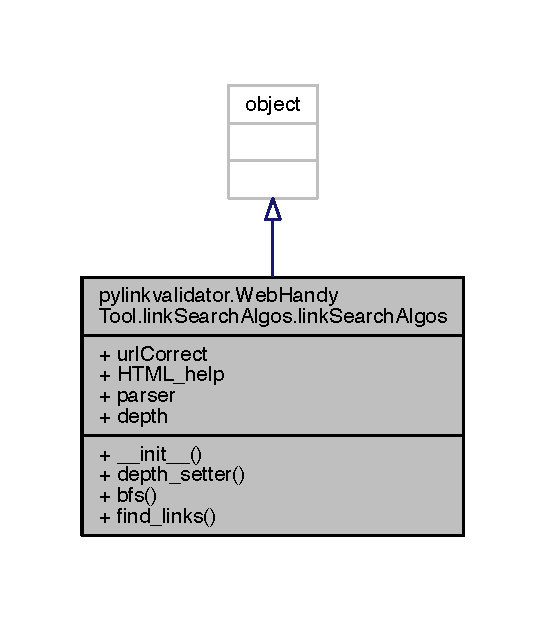
\includegraphics[width=262pt]{classpylinkvalidator_1_1_web_handy_tool_1_1link_search_algos_1_1link_search_algos__inherit__graph}
\end{center}
\end{figure}


Collaboration diagram for pylinkvalidator.\+Web\+Handy\+Tool.\+link\+Search\+Algos.\+link\+Search\+Algos\+:
\nopagebreak
\begin{figure}[H]
\begin{center}
\leavevmode
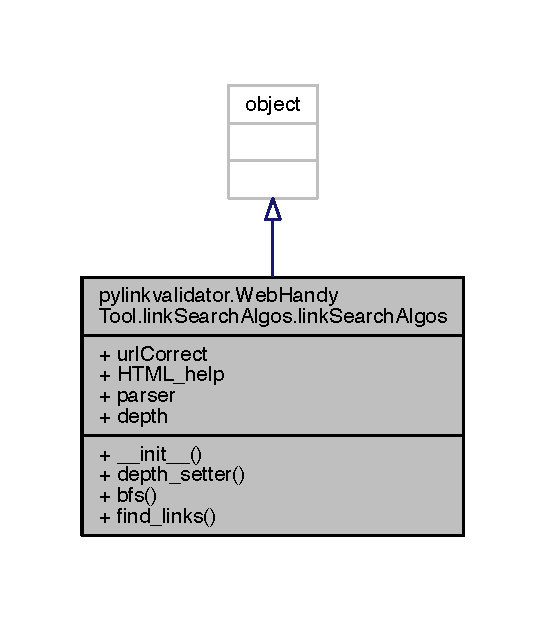
\includegraphics[width=262pt]{classpylinkvalidator_1_1_web_handy_tool_1_1link_search_algos_1_1link_search_algos__coll__graph}
\end{center}
\end{figure}
\subsection*{Public Member Functions}
\begin{DoxyCompactItemize}
\item 
def \hyperlink{classpylinkvalidator_1_1_web_handy_tool_1_1link_search_algos_1_1link_search_algos_a9aa0ef968fed3bf2cb5588a84658fa6c}{\+\_\+\+\_\+init\+\_\+\+\_\+} (self)
\item 
def \hyperlink{classpylinkvalidator_1_1_web_handy_tool_1_1link_search_algos_1_1link_search_algos_ad4cf802e4c3d47fc31b9d1e8e4c7c3d5}{depth\+\_\+setter} (self, \hyperlink{classpylinkvalidator_1_1_web_handy_tool_1_1link_search_algos_1_1link_search_algos_ab4bb72e4cdf3e63f85c88e49fe2abec6}{depth})
\item 
def \hyperlink{classpylinkvalidator_1_1_web_handy_tool_1_1link_search_algos_1_1link_search_algos_a3c4cb4d12b1850f7da9b84e612eac9bd}{bfs} (self, link)
\item 
def \hyperlink{classpylinkvalidator_1_1_web_handy_tool_1_1link_search_algos_1_1link_search_algos_aa4e7f6b9aa325f9cc21fe7aefd9ecad1}{find\+\_\+links} (self, link, destination=None)
\end{DoxyCompactItemize}
\subsection*{Public Attributes}
\begin{DoxyCompactItemize}
\item 
\hyperlink{classpylinkvalidator_1_1_web_handy_tool_1_1link_search_algos_1_1link_search_algos_adaaf5c989830ecfbdf552255678a0eb2}{url\+Correct}
\item 
\hyperlink{classpylinkvalidator_1_1_web_handy_tool_1_1link_search_algos_1_1link_search_algos_a8941e82772705f2e0462a628532075d1}{H\+T\+M\+L\+\_\+help}
\item 
\hyperlink{classpylinkvalidator_1_1_web_handy_tool_1_1link_search_algos_1_1link_search_algos_a326fd2c6dda6c9ecd87e7e09c2fdd2cc}{parser}
\item 
\hyperlink{classpylinkvalidator_1_1_web_handy_tool_1_1link_search_algos_1_1link_search_algos_ab4bb72e4cdf3e63f85c88e49fe2abec6}{depth}
\end{DoxyCompactItemize}


\subsection{Constructor \& Destructor Documentation}
\index{pylinkvalidator\+::\+Web\+Handy\+Tool\+::link\+Search\+Algos\+::link\+Search\+Algos@{pylinkvalidator\+::\+Web\+Handy\+Tool\+::link\+Search\+Algos\+::link\+Search\+Algos}!\+\_\+\+\_\+init\+\_\+\+\_\+@{\+\_\+\+\_\+init\+\_\+\+\_\+}}
\index{\+\_\+\+\_\+init\+\_\+\+\_\+@{\+\_\+\+\_\+init\+\_\+\+\_\+}!pylinkvalidator\+::\+Web\+Handy\+Tool\+::link\+Search\+Algos\+::link\+Search\+Algos@{pylinkvalidator\+::\+Web\+Handy\+Tool\+::link\+Search\+Algos\+::link\+Search\+Algos}}
\subsubsection[{\+\_\+\+\_\+init\+\_\+\+\_\+(self)}]{\setlength{\rightskip}{0pt plus 5cm}def pylinkvalidator.\+Web\+Handy\+Tool.\+link\+Search\+Algos.\+link\+Search\+Algos.\+\_\+\+\_\+init\+\_\+\+\_\+ (
\begin{DoxyParamCaption}
\item[{}]{self}
\end{DoxyParamCaption}
)}\hypertarget{classpylinkvalidator_1_1_web_handy_tool_1_1link_search_algos_1_1link_search_algos_a9aa0ef968fed3bf2cb5588a84658fa6c}{}\label{classpylinkvalidator_1_1_web_handy_tool_1_1link_search_algos_1_1link_search_algos_a9aa0ef968fed3bf2cb5588a84658fa6c}


\subsection{Member Function Documentation}
\index{pylinkvalidator\+::\+Web\+Handy\+Tool\+::link\+Search\+Algos\+::link\+Search\+Algos@{pylinkvalidator\+::\+Web\+Handy\+Tool\+::link\+Search\+Algos\+::link\+Search\+Algos}!bfs@{bfs}}
\index{bfs@{bfs}!pylinkvalidator\+::\+Web\+Handy\+Tool\+::link\+Search\+Algos\+::link\+Search\+Algos@{pylinkvalidator\+::\+Web\+Handy\+Tool\+::link\+Search\+Algos\+::link\+Search\+Algos}}
\subsubsection[{bfs(self, link)}]{\setlength{\rightskip}{0pt plus 5cm}def pylinkvalidator.\+Web\+Handy\+Tool.\+link\+Search\+Algos.\+link\+Search\+Algos.\+bfs (
\begin{DoxyParamCaption}
\item[{}]{self, }
\item[{}]{link}
\end{DoxyParamCaption}
)}\hypertarget{classpylinkvalidator_1_1_web_handy_tool_1_1link_search_algos_1_1link_search_algos_a3c4cb4d12b1850f7da9b84e612eac9bd}{}\label{classpylinkvalidator_1_1_web_handy_tool_1_1link_search_algos_1_1link_search_algos_a3c4cb4d12b1850f7da9b84e612eac9bd}
\begin{DoxyVerb}Finds all the links on a give website using the BFS algorithm
:param link:
:return A list of all the links found by BFS:
\end{DoxyVerb}
 

Here is the call graph for this function\+:
\nopagebreak
\begin{figure}[H]
\begin{center}
\leavevmode
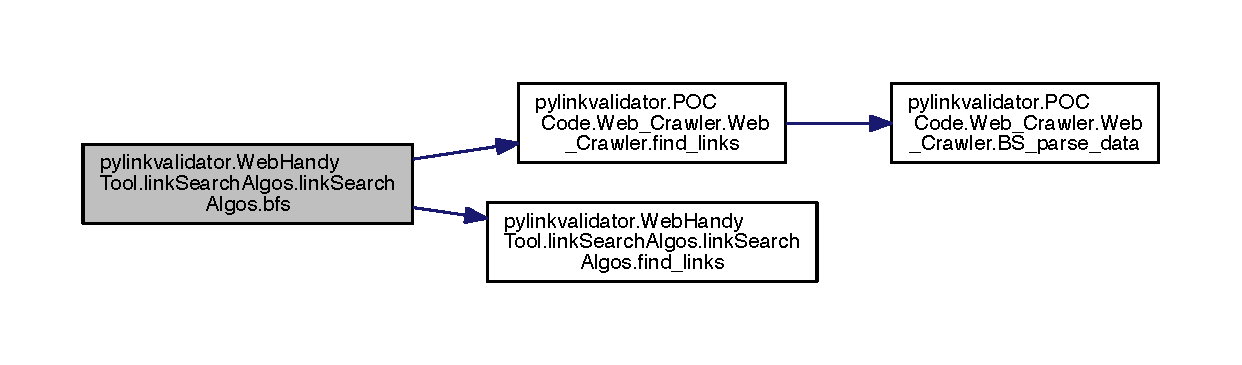
\includegraphics[width=350pt]{classpylinkvalidator_1_1_web_handy_tool_1_1link_search_algos_1_1link_search_algos_a3c4cb4d12b1850f7da9b84e612eac9bd_cgraph}
\end{center}
\end{figure}


\index{pylinkvalidator\+::\+Web\+Handy\+Tool\+::link\+Search\+Algos\+::link\+Search\+Algos@{pylinkvalidator\+::\+Web\+Handy\+Tool\+::link\+Search\+Algos\+::link\+Search\+Algos}!depth\+\_\+setter@{depth\+\_\+setter}}
\index{depth\+\_\+setter@{depth\+\_\+setter}!pylinkvalidator\+::\+Web\+Handy\+Tool\+::link\+Search\+Algos\+::link\+Search\+Algos@{pylinkvalidator\+::\+Web\+Handy\+Tool\+::link\+Search\+Algos\+::link\+Search\+Algos}}
\subsubsection[{depth\+\_\+setter(self, depth)}]{\setlength{\rightskip}{0pt plus 5cm}def pylinkvalidator.\+Web\+Handy\+Tool.\+link\+Search\+Algos.\+link\+Search\+Algos.\+depth\+\_\+setter (
\begin{DoxyParamCaption}
\item[{}]{self, }
\item[{}]{depth}
\end{DoxyParamCaption}
)}\hypertarget{classpylinkvalidator_1_1_web_handy_tool_1_1link_search_algos_1_1link_search_algos_ad4cf802e4c3d47fc31b9d1e8e4c7c3d5}{}\label{classpylinkvalidator_1_1_web_handy_tool_1_1link_search_algos_1_1link_search_algos_ad4cf802e4c3d47fc31b9d1e8e4c7c3d5}
\begin{DoxyVerb}Sets the default max depth variable for the web crawler
:param depth:
:return:
\end{DoxyVerb}
 \index{pylinkvalidator\+::\+Web\+Handy\+Tool\+::link\+Search\+Algos\+::link\+Search\+Algos@{pylinkvalidator\+::\+Web\+Handy\+Tool\+::link\+Search\+Algos\+::link\+Search\+Algos}!find\+\_\+links@{find\+\_\+links}}
\index{find\+\_\+links@{find\+\_\+links}!pylinkvalidator\+::\+Web\+Handy\+Tool\+::link\+Search\+Algos\+::link\+Search\+Algos@{pylinkvalidator\+::\+Web\+Handy\+Tool\+::link\+Search\+Algos\+::link\+Search\+Algos}}
\subsubsection[{find\+\_\+links(self, link, destination=\+None)}]{\setlength{\rightskip}{0pt plus 5cm}def pylinkvalidator.\+Web\+Handy\+Tool.\+link\+Search\+Algos.\+link\+Search\+Algos.\+find\+\_\+links (
\begin{DoxyParamCaption}
\item[{}]{self, }
\item[{}]{link, }
\item[{}]{destination = {\ttfamily None}}
\end{DoxyParamCaption}
)}\hypertarget{classpylinkvalidator_1_1_web_handy_tool_1_1link_search_algos_1_1link_search_algos_aa4e7f6b9aa325f9cc21fe7aefd9ecad1}{}\label{classpylinkvalidator_1_1_web_handy_tool_1_1link_search_algos_1_1link_search_algos_aa4e7f6b9aa325f9cc21fe7aefd9ecad1}
\begin{DoxyVerb}Finds all the links (<a></a> anchor tags on page) on a page, also removes all
the link that start with '#' or 'data:' as these are not valid urls

:param link:
:param destination:
:return List of Links:
\end{DoxyVerb}
 

Here is the caller graph for this function\+:
\nopagebreak
\begin{figure}[H]
\begin{center}
\leavevmode
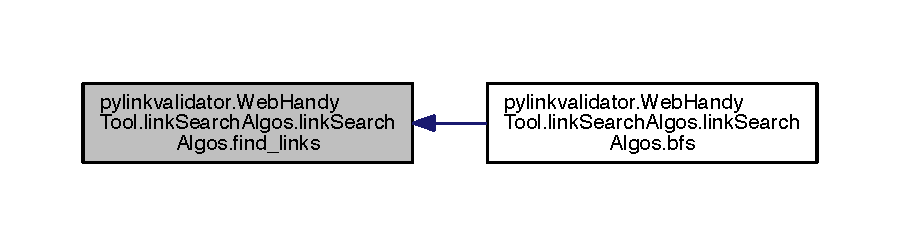
\includegraphics[width=350pt]{classpylinkvalidator_1_1_web_handy_tool_1_1link_search_algos_1_1link_search_algos_aa4e7f6b9aa325f9cc21fe7aefd9ecad1_icgraph}
\end{center}
\end{figure}




\subsection{Member Data Documentation}
\index{pylinkvalidator\+::\+Web\+Handy\+Tool\+::link\+Search\+Algos\+::link\+Search\+Algos@{pylinkvalidator\+::\+Web\+Handy\+Tool\+::link\+Search\+Algos\+::link\+Search\+Algos}!depth@{depth}}
\index{depth@{depth}!pylinkvalidator\+::\+Web\+Handy\+Tool\+::link\+Search\+Algos\+::link\+Search\+Algos@{pylinkvalidator\+::\+Web\+Handy\+Tool\+::link\+Search\+Algos\+::link\+Search\+Algos}}
\subsubsection[{depth}]{\setlength{\rightskip}{0pt plus 5cm}pylinkvalidator.\+Web\+Handy\+Tool.\+link\+Search\+Algos.\+link\+Search\+Algos.\+depth}\hypertarget{classpylinkvalidator_1_1_web_handy_tool_1_1link_search_algos_1_1link_search_algos_ab4bb72e4cdf3e63f85c88e49fe2abec6}{}\label{classpylinkvalidator_1_1_web_handy_tool_1_1link_search_algos_1_1link_search_algos_ab4bb72e4cdf3e63f85c88e49fe2abec6}
\index{pylinkvalidator\+::\+Web\+Handy\+Tool\+::link\+Search\+Algos\+::link\+Search\+Algos@{pylinkvalidator\+::\+Web\+Handy\+Tool\+::link\+Search\+Algos\+::link\+Search\+Algos}!H\+T\+M\+L\+\_\+help@{H\+T\+M\+L\+\_\+help}}
\index{H\+T\+M\+L\+\_\+help@{H\+T\+M\+L\+\_\+help}!pylinkvalidator\+::\+Web\+Handy\+Tool\+::link\+Search\+Algos\+::link\+Search\+Algos@{pylinkvalidator\+::\+Web\+Handy\+Tool\+::link\+Search\+Algos\+::link\+Search\+Algos}}
\subsubsection[{H\+T\+M\+L\+\_\+help}]{\setlength{\rightskip}{0pt plus 5cm}pylinkvalidator.\+Web\+Handy\+Tool.\+link\+Search\+Algos.\+link\+Search\+Algos.\+H\+T\+M\+L\+\_\+help}\hypertarget{classpylinkvalidator_1_1_web_handy_tool_1_1link_search_algos_1_1link_search_algos_a8941e82772705f2e0462a628532075d1}{}\label{classpylinkvalidator_1_1_web_handy_tool_1_1link_search_algos_1_1link_search_algos_a8941e82772705f2e0462a628532075d1}
\index{pylinkvalidator\+::\+Web\+Handy\+Tool\+::link\+Search\+Algos\+::link\+Search\+Algos@{pylinkvalidator\+::\+Web\+Handy\+Tool\+::link\+Search\+Algos\+::link\+Search\+Algos}!parser@{parser}}
\index{parser@{parser}!pylinkvalidator\+::\+Web\+Handy\+Tool\+::link\+Search\+Algos\+::link\+Search\+Algos@{pylinkvalidator\+::\+Web\+Handy\+Tool\+::link\+Search\+Algos\+::link\+Search\+Algos}}
\subsubsection[{parser}]{\setlength{\rightskip}{0pt plus 5cm}pylinkvalidator.\+Web\+Handy\+Tool.\+link\+Search\+Algos.\+link\+Search\+Algos.\+parser}\hypertarget{classpylinkvalidator_1_1_web_handy_tool_1_1link_search_algos_1_1link_search_algos_a326fd2c6dda6c9ecd87e7e09c2fdd2cc}{}\label{classpylinkvalidator_1_1_web_handy_tool_1_1link_search_algos_1_1link_search_algos_a326fd2c6dda6c9ecd87e7e09c2fdd2cc}
\index{pylinkvalidator\+::\+Web\+Handy\+Tool\+::link\+Search\+Algos\+::link\+Search\+Algos@{pylinkvalidator\+::\+Web\+Handy\+Tool\+::link\+Search\+Algos\+::link\+Search\+Algos}!url\+Correct@{url\+Correct}}
\index{url\+Correct@{url\+Correct}!pylinkvalidator\+::\+Web\+Handy\+Tool\+::link\+Search\+Algos\+::link\+Search\+Algos@{pylinkvalidator\+::\+Web\+Handy\+Tool\+::link\+Search\+Algos\+::link\+Search\+Algos}}
\subsubsection[{url\+Correct}]{\setlength{\rightskip}{0pt plus 5cm}pylinkvalidator.\+Web\+Handy\+Tool.\+link\+Search\+Algos.\+link\+Search\+Algos.\+url\+Correct}\hypertarget{classpylinkvalidator_1_1_web_handy_tool_1_1link_search_algos_1_1link_search_algos_adaaf5c989830ecfbdf552255678a0eb2}{}\label{classpylinkvalidator_1_1_web_handy_tool_1_1link_search_algos_1_1link_search_algos_adaaf5c989830ecfbdf552255678a0eb2}


The documentation for this class was generated from the following file\+:\begin{DoxyCompactItemize}
\item 
Web\+Handy\+Tool/\hyperlink{link_search_algos_8py}{link\+Search\+Algos.\+py}\end{DoxyCompactItemize}

\hypertarget{classpylinkvalidator_1_1_web_handy_tool_1_1parsers_1_1parsers}{}\section{pylinkvalidator.\+Web\+Handy\+Tool.\+parsers.\+parsers Class Reference}
\label{classpylinkvalidator_1_1_web_handy_tool_1_1parsers_1_1parsers}\index{pylinkvalidator.\+Web\+Handy\+Tool.\+parsers.\+parsers@{pylinkvalidator.\+Web\+Handy\+Tool.\+parsers.\+parsers}}


Inheritance diagram for pylinkvalidator.\+Web\+Handy\+Tool.\+parsers.\+parsers\+:
\nopagebreak
\begin{figure}[H]
\begin{center}
\leavevmode
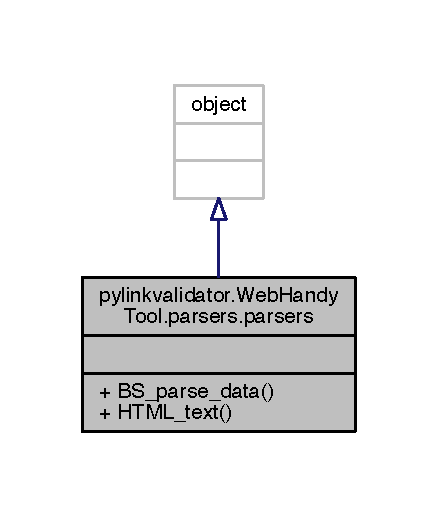
\includegraphics[width=210pt]{classpylinkvalidator_1_1_web_handy_tool_1_1parsers_1_1parsers__inherit__graph}
\end{center}
\end{figure}


Collaboration diagram for pylinkvalidator.\+Web\+Handy\+Tool.\+parsers.\+parsers\+:
\nopagebreak
\begin{figure}[H]
\begin{center}
\leavevmode
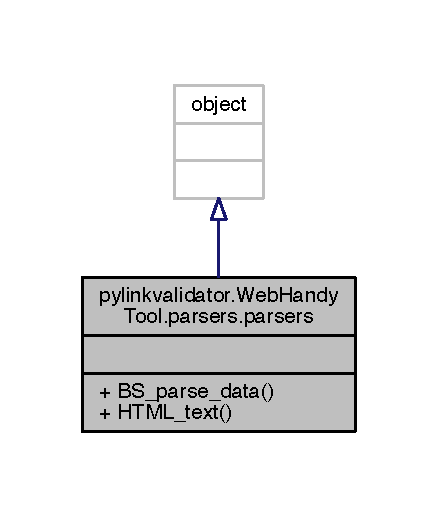
\includegraphics[width=210pt]{classpylinkvalidator_1_1_web_handy_tool_1_1parsers_1_1parsers__coll__graph}
\end{center}
\end{figure}
\subsection*{Public Member Functions}
\begin{DoxyCompactItemize}
\item 
def \hyperlink{classpylinkvalidator_1_1_web_handy_tool_1_1parsers_1_1parsers_ac6c458e5f64a0cddded5782799aa0a3f}{B\+S\+\_\+parse\+\_\+data} (self, link)
\item 
def \hyperlink{classpylinkvalidator_1_1_web_handy_tool_1_1parsers_1_1parsers_a8145b02d268056ef0153e42ea4a0aa70}{H\+T\+M\+L\+\_\+text} (self, link)
\end{DoxyCompactItemize}


\subsection{Member Function Documentation}
\index{pylinkvalidator\+::\+Web\+Handy\+Tool\+::parsers\+::parsers@{pylinkvalidator\+::\+Web\+Handy\+Tool\+::parsers\+::parsers}!B\+S\+\_\+parse\+\_\+data@{B\+S\+\_\+parse\+\_\+data}}
\index{B\+S\+\_\+parse\+\_\+data@{B\+S\+\_\+parse\+\_\+data}!pylinkvalidator\+::\+Web\+Handy\+Tool\+::parsers\+::parsers@{pylinkvalidator\+::\+Web\+Handy\+Tool\+::parsers\+::parsers}}
\subsubsection[{B\+S\+\_\+parse\+\_\+data(self, link)}]{\setlength{\rightskip}{0pt plus 5cm}def pylinkvalidator.\+Web\+Handy\+Tool.\+parsers.\+parsers.\+B\+S\+\_\+parse\+\_\+data (
\begin{DoxyParamCaption}
\item[{}]{self, }
\item[{}]{link}
\end{DoxyParamCaption}
)}\hypertarget{classpylinkvalidator_1_1_web_handy_tool_1_1parsers_1_1parsers_ac6c458e5f64a0cddded5782799aa0a3f}{}\label{classpylinkvalidator_1_1_web_handy_tool_1_1parsers_1_1parsers_ac6c458e5f64a0cddded5782799aa0a3f}
\begin{DoxyVerb}Returns BeautifulSoup object for the link given, this will allow modules parse through pages data much faster

:param link:
:return BeautifulSoup :
\end{DoxyVerb}
 \index{pylinkvalidator\+::\+Web\+Handy\+Tool\+::parsers\+::parsers@{pylinkvalidator\+::\+Web\+Handy\+Tool\+::parsers\+::parsers}!H\+T\+M\+L\+\_\+text@{H\+T\+M\+L\+\_\+text}}
\index{H\+T\+M\+L\+\_\+text@{H\+T\+M\+L\+\_\+text}!pylinkvalidator\+::\+Web\+Handy\+Tool\+::parsers\+::parsers@{pylinkvalidator\+::\+Web\+Handy\+Tool\+::parsers\+::parsers}}
\subsubsection[{H\+T\+M\+L\+\_\+text(self, link)}]{\setlength{\rightskip}{0pt plus 5cm}def pylinkvalidator.\+Web\+Handy\+Tool.\+parsers.\+parsers.\+H\+T\+M\+L\+\_\+text (
\begin{DoxyParamCaption}
\item[{}]{self, }
\item[{}]{link}
\end{DoxyParamCaption}
)}\hypertarget{classpylinkvalidator_1_1_web_handy_tool_1_1parsers_1_1parsers_a8145b02d268056ef0153e42ea4a0aa70}{}\label{classpylinkvalidator_1_1_web_handy_tool_1_1parsers_1_1parsers_a8145b02d268056ef0153e42ea4a0aa70}
\begin{DoxyVerb}Returns HTML text data for Query search

:param link:
:return String :
\end{DoxyVerb}
 

The documentation for this class was generated from the following file\+:\begin{DoxyCompactItemize}
\item 
Web\+Handy\+Tool/\hyperlink{parsers_8py}{parsers.\+py}\end{DoxyCompactItemize}

\hypertarget{classpylinkvalidator_1_1_web_handy_tool_1_1search_1_1search}{}\section{pylinkvalidator.\+Web\+Handy\+Tool.\+search.\+search Class Reference}
\label{classpylinkvalidator_1_1_web_handy_tool_1_1search_1_1search}\index{pylinkvalidator.\+Web\+Handy\+Tool.\+search.\+search@{pylinkvalidator.\+Web\+Handy\+Tool.\+search.\+search}}


Inheritance diagram for pylinkvalidator.\+Web\+Handy\+Tool.\+search.\+search\+:
\nopagebreak
\begin{figure}[H]
\begin{center}
\leavevmode
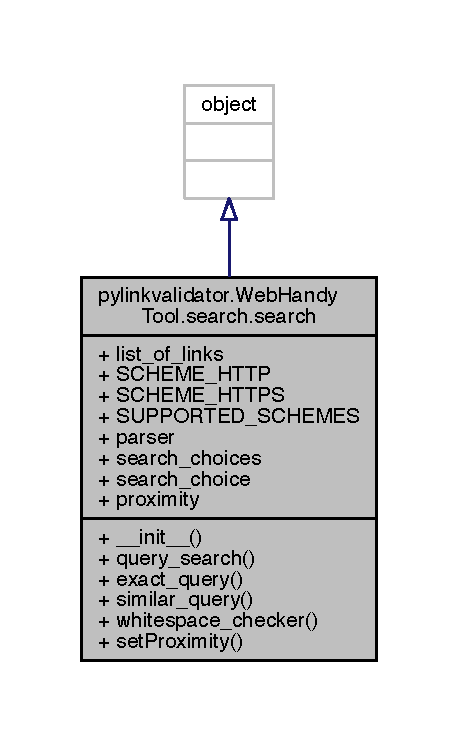
\includegraphics[width=220pt]{classpylinkvalidator_1_1_web_handy_tool_1_1search_1_1search__inherit__graph}
\end{center}
\end{figure}


Collaboration diagram for pylinkvalidator.\+Web\+Handy\+Tool.\+search.\+search\+:
\nopagebreak
\begin{figure}[H]
\begin{center}
\leavevmode
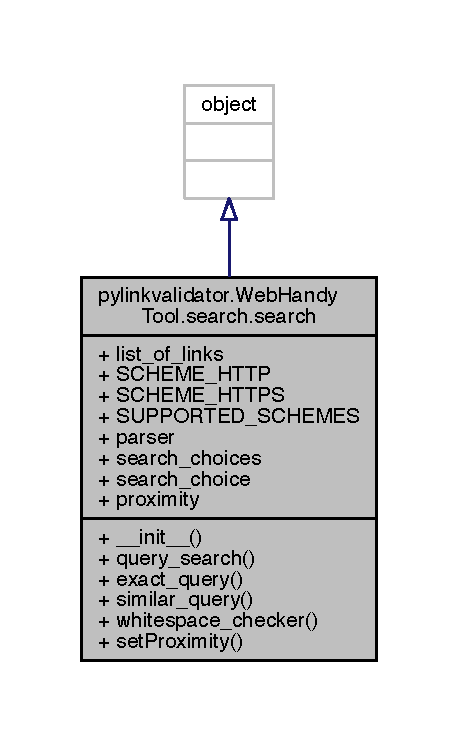
\includegraphics[width=220pt]{classpylinkvalidator_1_1_web_handy_tool_1_1search_1_1search__coll__graph}
\end{center}
\end{figure}
\subsection*{Public Member Functions}
\begin{DoxyCompactItemize}
\item 
def \hyperlink{classpylinkvalidator_1_1_web_handy_tool_1_1search_1_1search_a938adf672af9ce7a03aa3f1dfc1a4148}{\+\_\+\+\_\+init\+\_\+\+\_\+} (self)
\item 
def \hyperlink{classpylinkvalidator_1_1_web_handy_tool_1_1search_1_1search_aed98782e4a3538c3be75eeb3af8050e5}{query\+\_\+search} (self, query, link, \hyperlink{classpylinkvalidator_1_1_web_handy_tool_1_1search_1_1search_a906e019972fbdaef6ef37b50edc2cb1f}{list\+\_\+of\+\_\+links}=None, choice=\textquotesingle{}exact\textquotesingle{})
\item 
def \hyperlink{classpylinkvalidator_1_1_web_handy_tool_1_1search_1_1search_a2f6e5ce0d893c396139877a60b34d8e9}{exact\+\_\+query} (self, query, data)
\item 
def \hyperlink{classpylinkvalidator_1_1_web_handy_tool_1_1search_1_1search_ad8279fa98fb80bfaae0800cd7c5fa21e}{similar\+\_\+query} (self, query, data, \hyperlink{classpylinkvalidator_1_1_web_handy_tool_1_1search_1_1search_ad4742d4d507c4ea17dd4f4b5881047db}{proximity})
\item 
def \hyperlink{classpylinkvalidator_1_1_web_handy_tool_1_1search_1_1search_a95044af0828393b590c4946fe8aa16b5}{whitespace\+\_\+checker} (self, character)
\item 
def \hyperlink{classpylinkvalidator_1_1_web_handy_tool_1_1search_1_1search_a3070944be3de739d70f8c4c4603cbf4a}{set\+Proximity} (self, \hyperlink{classpylinkvalidator_1_1_web_handy_tool_1_1search_1_1search_ad4742d4d507c4ea17dd4f4b5881047db}{proximity})
\end{DoxyCompactItemize}
\subsection*{Public Attributes}
\begin{DoxyCompactItemize}
\item 
\hyperlink{classpylinkvalidator_1_1_web_handy_tool_1_1search_1_1search_a906e019972fbdaef6ef37b50edc2cb1f}{list\+\_\+of\+\_\+links}
\item 
\hyperlink{classpylinkvalidator_1_1_web_handy_tool_1_1search_1_1search_a31e3b450f5d912acbd1023535bef5599}{S\+C\+H\+E\+M\+E\+\_\+\+H\+T\+TP}
\item 
\hyperlink{classpylinkvalidator_1_1_web_handy_tool_1_1search_1_1search_a8827d73fa0682f75372ea6ca6a74fc48}{S\+C\+H\+E\+M\+E\+\_\+\+H\+T\+T\+PS}
\item 
\hyperlink{classpylinkvalidator_1_1_web_handy_tool_1_1search_1_1search_a40286fb518de4e5067f92d1b65870cf5}{S\+U\+P\+P\+O\+R\+T\+E\+D\+\_\+\+S\+C\+H\+E\+M\+ES}
\item 
\hyperlink{classpylinkvalidator_1_1_web_handy_tool_1_1search_1_1search_ad36362c5105b91945b7aa63b16f237c1}{parser}
\item 
\hyperlink{classpylinkvalidator_1_1_web_handy_tool_1_1search_1_1search_a6d89cd65d2a2103906c1b72acfdc35a2}{search\+\_\+choices}
\item 
\hyperlink{classpylinkvalidator_1_1_web_handy_tool_1_1search_1_1search_a8aad3e0ea9b36c98f84fd6f192fb12e7}{search\+\_\+choice}
\item 
\hyperlink{classpylinkvalidator_1_1_web_handy_tool_1_1search_1_1search_ad4742d4d507c4ea17dd4f4b5881047db}{proximity}
\end{DoxyCompactItemize}


\subsection{Constructor \& Destructor Documentation}
\index{pylinkvalidator\+::\+Web\+Handy\+Tool\+::search\+::search@{pylinkvalidator\+::\+Web\+Handy\+Tool\+::search\+::search}!\+\_\+\+\_\+init\+\_\+\+\_\+@{\+\_\+\+\_\+init\+\_\+\+\_\+}}
\index{\+\_\+\+\_\+init\+\_\+\+\_\+@{\+\_\+\+\_\+init\+\_\+\+\_\+}!pylinkvalidator\+::\+Web\+Handy\+Tool\+::search\+::search@{pylinkvalidator\+::\+Web\+Handy\+Tool\+::search\+::search}}
\subsubsection[{\+\_\+\+\_\+init\+\_\+\+\_\+(self)}]{\setlength{\rightskip}{0pt plus 5cm}def pylinkvalidator.\+Web\+Handy\+Tool.\+search.\+search.\+\_\+\+\_\+init\+\_\+\+\_\+ (
\begin{DoxyParamCaption}
\item[{}]{self}
\end{DoxyParamCaption}
)}\hypertarget{classpylinkvalidator_1_1_web_handy_tool_1_1search_1_1search_a938adf672af9ce7a03aa3f1dfc1a4148}{}\label{classpylinkvalidator_1_1_web_handy_tool_1_1search_1_1search_a938adf672af9ce7a03aa3f1dfc1a4148}


\subsection{Member Function Documentation}
\index{pylinkvalidator\+::\+Web\+Handy\+Tool\+::search\+::search@{pylinkvalidator\+::\+Web\+Handy\+Tool\+::search\+::search}!exact\+\_\+query@{exact\+\_\+query}}
\index{exact\+\_\+query@{exact\+\_\+query}!pylinkvalidator\+::\+Web\+Handy\+Tool\+::search\+::search@{pylinkvalidator\+::\+Web\+Handy\+Tool\+::search\+::search}}
\subsubsection[{exact\+\_\+query(self, query, data)}]{\setlength{\rightskip}{0pt plus 5cm}def pylinkvalidator.\+Web\+Handy\+Tool.\+search.\+search.\+exact\+\_\+query (
\begin{DoxyParamCaption}
\item[{}]{self, }
\item[{}]{query, }
\item[{}]{data}
\end{DoxyParamCaption}
)}\hypertarget{classpylinkvalidator_1_1_web_handy_tool_1_1search_1_1search_a2f6e5ce0d893c396139877a60b34d8e9}{}\label{classpylinkvalidator_1_1_web_handy_tool_1_1search_1_1search_a2f6e5ce0d893c396139877a60b34d8e9}
\begin{DoxyVerb}Searches through a String for a certain phrase or term. Returns the starting index for all occurrences of the query String.
If the query is not located, it will return an empty array.

:param query - The String we are looking for:
:param data - The String we are searching through.:
:return Indexes corresponding to the beginning of the location of the String in question.:
\end{DoxyVerb}
 

Here is the caller graph for this function\+:
\nopagebreak
\begin{figure}[H]
\begin{center}
\leavevmode
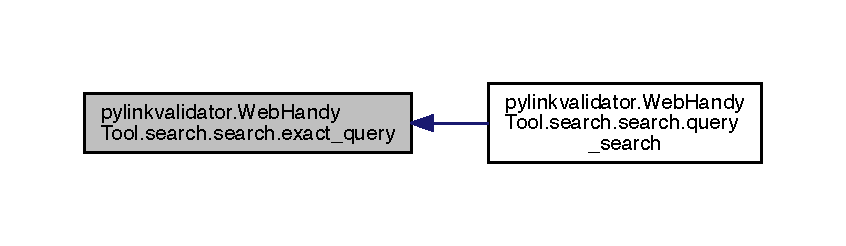
\includegraphics[width=350pt]{classpylinkvalidator_1_1_web_handy_tool_1_1search_1_1search_a2f6e5ce0d893c396139877a60b34d8e9_icgraph}
\end{center}
\end{figure}


\index{pylinkvalidator\+::\+Web\+Handy\+Tool\+::search\+::search@{pylinkvalidator\+::\+Web\+Handy\+Tool\+::search\+::search}!query\+\_\+search@{query\+\_\+search}}
\index{query\+\_\+search@{query\+\_\+search}!pylinkvalidator\+::\+Web\+Handy\+Tool\+::search\+::search@{pylinkvalidator\+::\+Web\+Handy\+Tool\+::search\+::search}}
\subsubsection[{query\+\_\+search(self, query, link, list\+\_\+of\+\_\+links=\+None, choice=\textquotesingle{}exact\textquotesingle{})}]{\setlength{\rightskip}{0pt plus 5cm}def pylinkvalidator.\+Web\+Handy\+Tool.\+search.\+search.\+query\+\_\+search (
\begin{DoxyParamCaption}
\item[{}]{self, }
\item[{}]{query, }
\item[{}]{link, }
\item[{}]{list\+\_\+of\+\_\+links = {\ttfamily None}, }
\item[{}]{choice = {\ttfamily \textquotesingle{}exact\textquotesingle{}}}
\end{DoxyParamCaption}
)}\hypertarget{classpylinkvalidator_1_1_web_handy_tool_1_1search_1_1search_aed98782e4a3538c3be75eeb3af8050e5}{}\label{classpylinkvalidator_1_1_web_handy_tool_1_1search_1_1search_aed98782e4a3538c3be75eeb3af8050e5}
\begin{DoxyVerb}Find queries

:param query:
:param data:
:param choice:
:return Query results:
\end{DoxyVerb}
 

Here is the call graph for this function\+:
\nopagebreak
\begin{figure}[H]
\begin{center}
\leavevmode
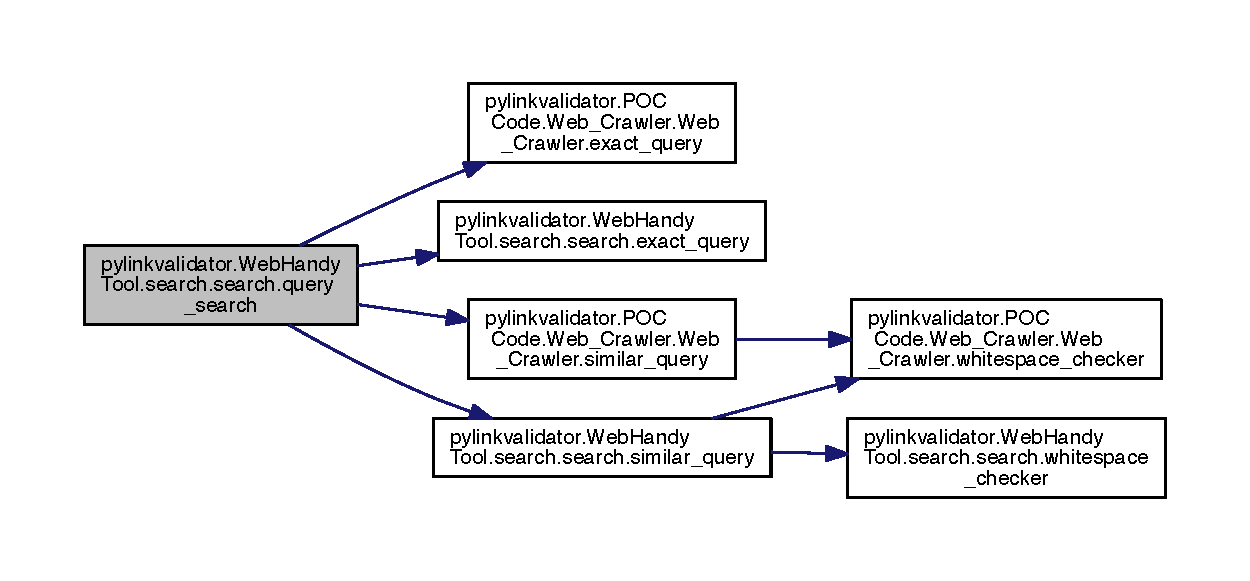
\includegraphics[width=350pt]{classpylinkvalidator_1_1_web_handy_tool_1_1search_1_1search_aed98782e4a3538c3be75eeb3af8050e5_cgraph}
\end{center}
\end{figure}


\index{pylinkvalidator\+::\+Web\+Handy\+Tool\+::search\+::search@{pylinkvalidator\+::\+Web\+Handy\+Tool\+::search\+::search}!set\+Proximity@{set\+Proximity}}
\index{set\+Proximity@{set\+Proximity}!pylinkvalidator\+::\+Web\+Handy\+Tool\+::search\+::search@{pylinkvalidator\+::\+Web\+Handy\+Tool\+::search\+::search}}
\subsubsection[{set\+Proximity(self, proximity)}]{\setlength{\rightskip}{0pt plus 5cm}def pylinkvalidator.\+Web\+Handy\+Tool.\+search.\+search.\+set\+Proximity (
\begin{DoxyParamCaption}
\item[{}]{self, }
\item[{}]{proximity}
\end{DoxyParamCaption}
)}\hypertarget{classpylinkvalidator_1_1_web_handy_tool_1_1search_1_1search_a3070944be3de739d70f8c4c4603cbf4a}{}\label{classpylinkvalidator_1_1_web_handy_tool_1_1search_1_1search_a3070944be3de739d70f8c4c4603cbf4a}
\begin{DoxyVerb}Set the search proximity
:param proximity:
:return:
\end{DoxyVerb}
 \index{pylinkvalidator\+::\+Web\+Handy\+Tool\+::search\+::search@{pylinkvalidator\+::\+Web\+Handy\+Tool\+::search\+::search}!similar\+\_\+query@{similar\+\_\+query}}
\index{similar\+\_\+query@{similar\+\_\+query}!pylinkvalidator\+::\+Web\+Handy\+Tool\+::search\+::search@{pylinkvalidator\+::\+Web\+Handy\+Tool\+::search\+::search}}
\subsubsection[{similar\+\_\+query(self, query, data, proximity)}]{\setlength{\rightskip}{0pt plus 5cm}def pylinkvalidator.\+Web\+Handy\+Tool.\+search.\+search.\+similar\+\_\+query (
\begin{DoxyParamCaption}
\item[{}]{self, }
\item[{}]{query, }
\item[{}]{data, }
\item[{}]{proximity}
\end{DoxyParamCaption}
)}\hypertarget{classpylinkvalidator_1_1_web_handy_tool_1_1search_1_1search_ad8279fa98fb80bfaae0800cd7c5fa21e}{}\label{classpylinkvalidator_1_1_web_handy_tool_1_1search_1_1search_ad8279fa98fb80bfaae0800cd7c5fa21e}
\begin{DoxyVerb}Searches through a String for a certain phrase or term. Returns results that are close to the query as well.
(i.e. "ap ple" or "bpple" would be noted for "apple") Returns the starting index for all occurrences of Strings sufficiently close to
the query. If the query is not located, it will return an empty array.

:param: query  - The String we are looking for.
:param: data - The String we are searching through.:
:param: proximity - The size of the acceptable variation from the query.:
:return:Indexes corresponding to the beginning of the location of the String in question.
\end{DoxyVerb}
 

Here is the call graph for this function\+:
\nopagebreak
\begin{figure}[H]
\begin{center}
\leavevmode
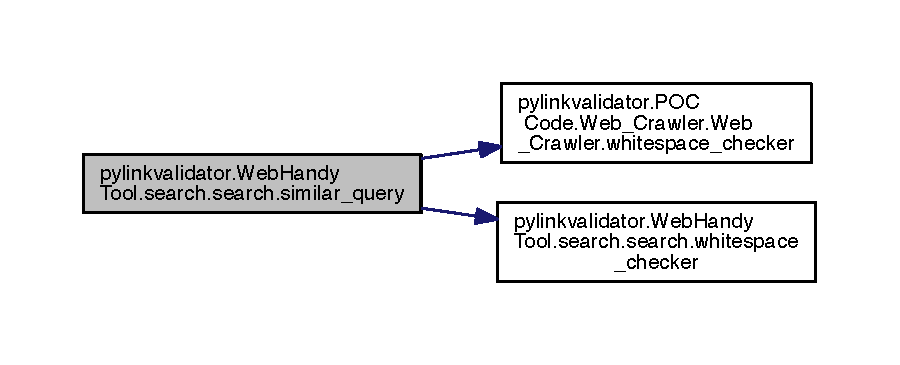
\includegraphics[width=350pt]{classpylinkvalidator_1_1_web_handy_tool_1_1search_1_1search_ad8279fa98fb80bfaae0800cd7c5fa21e_cgraph}
\end{center}
\end{figure}




Here is the caller graph for this function\+:
\nopagebreak
\begin{figure}[H]
\begin{center}
\leavevmode
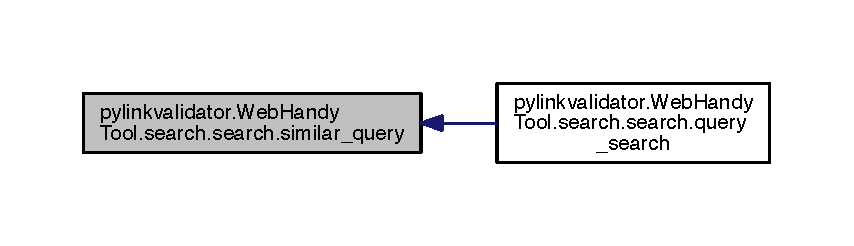
\includegraphics[width=350pt]{classpylinkvalidator_1_1_web_handy_tool_1_1search_1_1search_ad8279fa98fb80bfaae0800cd7c5fa21e_icgraph}
\end{center}
\end{figure}


\index{pylinkvalidator\+::\+Web\+Handy\+Tool\+::search\+::search@{pylinkvalidator\+::\+Web\+Handy\+Tool\+::search\+::search}!whitespace\+\_\+checker@{whitespace\+\_\+checker}}
\index{whitespace\+\_\+checker@{whitespace\+\_\+checker}!pylinkvalidator\+::\+Web\+Handy\+Tool\+::search\+::search@{pylinkvalidator\+::\+Web\+Handy\+Tool\+::search\+::search}}
\subsubsection[{whitespace\+\_\+checker(self, character)}]{\setlength{\rightskip}{0pt plus 5cm}def pylinkvalidator.\+Web\+Handy\+Tool.\+search.\+search.\+whitespace\+\_\+checker (
\begin{DoxyParamCaption}
\item[{}]{self, }
\item[{}]{character}
\end{DoxyParamCaption}
)}\hypertarget{classpylinkvalidator_1_1_web_handy_tool_1_1search_1_1search_a95044af0828393b590c4946fe8aa16b5}{}\label{classpylinkvalidator_1_1_web_handy_tool_1_1search_1_1search_a95044af0828393b590c4946fe8aa16b5}
\begin{DoxyVerb}Returns true if the character passed in is a whitespace character such as tab, space or newline.

:param character - The character to be checked.:
:return boolean, if there is whitespace True,Whether the character is whitespace:
\end{DoxyVerb}
 

Here is the caller graph for this function\+:
\nopagebreak
\begin{figure}[H]
\begin{center}
\leavevmode
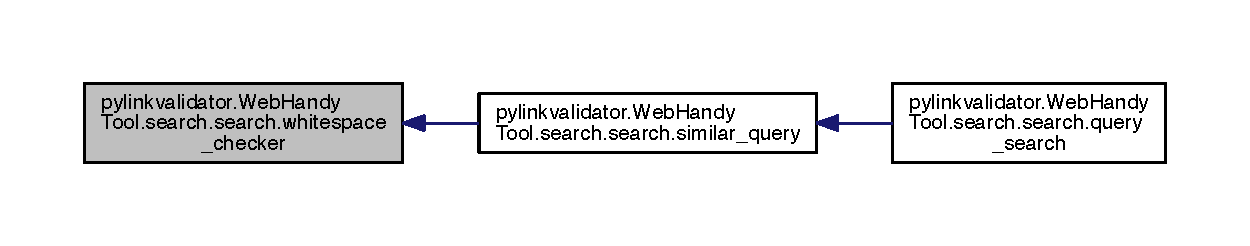
\includegraphics[width=350pt]{classpylinkvalidator_1_1_web_handy_tool_1_1search_1_1search_a95044af0828393b590c4946fe8aa16b5_icgraph}
\end{center}
\end{figure}




\subsection{Member Data Documentation}
\index{pylinkvalidator\+::\+Web\+Handy\+Tool\+::search\+::search@{pylinkvalidator\+::\+Web\+Handy\+Tool\+::search\+::search}!list\+\_\+of\+\_\+links@{list\+\_\+of\+\_\+links}}
\index{list\+\_\+of\+\_\+links@{list\+\_\+of\+\_\+links}!pylinkvalidator\+::\+Web\+Handy\+Tool\+::search\+::search@{pylinkvalidator\+::\+Web\+Handy\+Tool\+::search\+::search}}
\subsubsection[{list\+\_\+of\+\_\+links}]{\setlength{\rightskip}{0pt plus 5cm}pylinkvalidator.\+Web\+Handy\+Tool.\+search.\+search.\+list\+\_\+of\+\_\+links}\hypertarget{classpylinkvalidator_1_1_web_handy_tool_1_1search_1_1search_a906e019972fbdaef6ef37b50edc2cb1f}{}\label{classpylinkvalidator_1_1_web_handy_tool_1_1search_1_1search_a906e019972fbdaef6ef37b50edc2cb1f}
\index{pylinkvalidator\+::\+Web\+Handy\+Tool\+::search\+::search@{pylinkvalidator\+::\+Web\+Handy\+Tool\+::search\+::search}!parser@{parser}}
\index{parser@{parser}!pylinkvalidator\+::\+Web\+Handy\+Tool\+::search\+::search@{pylinkvalidator\+::\+Web\+Handy\+Tool\+::search\+::search}}
\subsubsection[{parser}]{\setlength{\rightskip}{0pt plus 5cm}pylinkvalidator.\+Web\+Handy\+Tool.\+search.\+search.\+parser}\hypertarget{classpylinkvalidator_1_1_web_handy_tool_1_1search_1_1search_ad36362c5105b91945b7aa63b16f237c1}{}\label{classpylinkvalidator_1_1_web_handy_tool_1_1search_1_1search_ad36362c5105b91945b7aa63b16f237c1}
\index{pylinkvalidator\+::\+Web\+Handy\+Tool\+::search\+::search@{pylinkvalidator\+::\+Web\+Handy\+Tool\+::search\+::search}!proximity@{proximity}}
\index{proximity@{proximity}!pylinkvalidator\+::\+Web\+Handy\+Tool\+::search\+::search@{pylinkvalidator\+::\+Web\+Handy\+Tool\+::search\+::search}}
\subsubsection[{proximity}]{\setlength{\rightskip}{0pt plus 5cm}pylinkvalidator.\+Web\+Handy\+Tool.\+search.\+search.\+proximity}\hypertarget{classpylinkvalidator_1_1_web_handy_tool_1_1search_1_1search_ad4742d4d507c4ea17dd4f4b5881047db}{}\label{classpylinkvalidator_1_1_web_handy_tool_1_1search_1_1search_ad4742d4d507c4ea17dd4f4b5881047db}
\index{pylinkvalidator\+::\+Web\+Handy\+Tool\+::search\+::search@{pylinkvalidator\+::\+Web\+Handy\+Tool\+::search\+::search}!S\+C\+H\+E\+M\+E\+\_\+\+H\+T\+TP@{S\+C\+H\+E\+M\+E\+\_\+\+H\+T\+TP}}
\index{S\+C\+H\+E\+M\+E\+\_\+\+H\+T\+TP@{S\+C\+H\+E\+M\+E\+\_\+\+H\+T\+TP}!pylinkvalidator\+::\+Web\+Handy\+Tool\+::search\+::search@{pylinkvalidator\+::\+Web\+Handy\+Tool\+::search\+::search}}
\subsubsection[{S\+C\+H\+E\+M\+E\+\_\+\+H\+T\+TP}]{\setlength{\rightskip}{0pt plus 5cm}pylinkvalidator.\+Web\+Handy\+Tool.\+search.\+search.\+S\+C\+H\+E\+M\+E\+\_\+\+H\+T\+TP}\hypertarget{classpylinkvalidator_1_1_web_handy_tool_1_1search_1_1search_a31e3b450f5d912acbd1023535bef5599}{}\label{classpylinkvalidator_1_1_web_handy_tool_1_1search_1_1search_a31e3b450f5d912acbd1023535bef5599}
\index{pylinkvalidator\+::\+Web\+Handy\+Tool\+::search\+::search@{pylinkvalidator\+::\+Web\+Handy\+Tool\+::search\+::search}!S\+C\+H\+E\+M\+E\+\_\+\+H\+T\+T\+PS@{S\+C\+H\+E\+M\+E\+\_\+\+H\+T\+T\+PS}}
\index{S\+C\+H\+E\+M\+E\+\_\+\+H\+T\+T\+PS@{S\+C\+H\+E\+M\+E\+\_\+\+H\+T\+T\+PS}!pylinkvalidator\+::\+Web\+Handy\+Tool\+::search\+::search@{pylinkvalidator\+::\+Web\+Handy\+Tool\+::search\+::search}}
\subsubsection[{S\+C\+H\+E\+M\+E\+\_\+\+H\+T\+T\+PS}]{\setlength{\rightskip}{0pt plus 5cm}pylinkvalidator.\+Web\+Handy\+Tool.\+search.\+search.\+S\+C\+H\+E\+M\+E\+\_\+\+H\+T\+T\+PS}\hypertarget{classpylinkvalidator_1_1_web_handy_tool_1_1search_1_1search_a8827d73fa0682f75372ea6ca6a74fc48}{}\label{classpylinkvalidator_1_1_web_handy_tool_1_1search_1_1search_a8827d73fa0682f75372ea6ca6a74fc48}
\index{pylinkvalidator\+::\+Web\+Handy\+Tool\+::search\+::search@{pylinkvalidator\+::\+Web\+Handy\+Tool\+::search\+::search}!search\+\_\+choice@{search\+\_\+choice}}
\index{search\+\_\+choice@{search\+\_\+choice}!pylinkvalidator\+::\+Web\+Handy\+Tool\+::search\+::search@{pylinkvalidator\+::\+Web\+Handy\+Tool\+::search\+::search}}
\subsubsection[{search\+\_\+choice}]{\setlength{\rightskip}{0pt plus 5cm}pylinkvalidator.\+Web\+Handy\+Tool.\+search.\+search.\+search\+\_\+choice}\hypertarget{classpylinkvalidator_1_1_web_handy_tool_1_1search_1_1search_a8aad3e0ea9b36c98f84fd6f192fb12e7}{}\label{classpylinkvalidator_1_1_web_handy_tool_1_1search_1_1search_a8aad3e0ea9b36c98f84fd6f192fb12e7}
\index{pylinkvalidator\+::\+Web\+Handy\+Tool\+::search\+::search@{pylinkvalidator\+::\+Web\+Handy\+Tool\+::search\+::search}!search\+\_\+choices@{search\+\_\+choices}}
\index{search\+\_\+choices@{search\+\_\+choices}!pylinkvalidator\+::\+Web\+Handy\+Tool\+::search\+::search@{pylinkvalidator\+::\+Web\+Handy\+Tool\+::search\+::search}}
\subsubsection[{search\+\_\+choices}]{\setlength{\rightskip}{0pt plus 5cm}pylinkvalidator.\+Web\+Handy\+Tool.\+search.\+search.\+search\+\_\+choices}\hypertarget{classpylinkvalidator_1_1_web_handy_tool_1_1search_1_1search_a6d89cd65d2a2103906c1b72acfdc35a2}{}\label{classpylinkvalidator_1_1_web_handy_tool_1_1search_1_1search_a6d89cd65d2a2103906c1b72acfdc35a2}
\index{pylinkvalidator\+::\+Web\+Handy\+Tool\+::search\+::search@{pylinkvalidator\+::\+Web\+Handy\+Tool\+::search\+::search}!S\+U\+P\+P\+O\+R\+T\+E\+D\+\_\+\+S\+C\+H\+E\+M\+ES@{S\+U\+P\+P\+O\+R\+T\+E\+D\+\_\+\+S\+C\+H\+E\+M\+ES}}
\index{S\+U\+P\+P\+O\+R\+T\+E\+D\+\_\+\+S\+C\+H\+E\+M\+ES@{S\+U\+P\+P\+O\+R\+T\+E\+D\+\_\+\+S\+C\+H\+E\+M\+ES}!pylinkvalidator\+::\+Web\+Handy\+Tool\+::search\+::search@{pylinkvalidator\+::\+Web\+Handy\+Tool\+::search\+::search}}
\subsubsection[{S\+U\+P\+P\+O\+R\+T\+E\+D\+\_\+\+S\+C\+H\+E\+M\+ES}]{\setlength{\rightskip}{0pt plus 5cm}pylinkvalidator.\+Web\+Handy\+Tool.\+search.\+search.\+S\+U\+P\+P\+O\+R\+T\+E\+D\+\_\+\+S\+C\+H\+E\+M\+ES}\hypertarget{classpylinkvalidator_1_1_web_handy_tool_1_1search_1_1search_a40286fb518de4e5067f92d1b65870cf5}{}\label{classpylinkvalidator_1_1_web_handy_tool_1_1search_1_1search_a40286fb518de4e5067f92d1b65870cf5}


The documentation for this class was generated from the following file\+:\begin{DoxyCompactItemize}
\item 
Web\+Handy\+Tool/\hyperlink{search_8py}{search.\+py}\end{DoxyCompactItemize}

\hypertarget{classpylinkvalidator_1_1_web_handy_tool_1_1tests_1_1search_test}{}\section{pylinkvalidator.\+Web\+Handy\+Tool.\+tests.\+search\+Test Class Reference}
\label{classpylinkvalidator_1_1_web_handy_tool_1_1tests_1_1search_test}\index{pylinkvalidator.\+Web\+Handy\+Tool.\+tests.\+search\+Test@{pylinkvalidator.\+Web\+Handy\+Tool.\+tests.\+search\+Test}}


Inheritance diagram for pylinkvalidator.\+Web\+Handy\+Tool.\+tests.\+search\+Test\+:
\nopagebreak
\begin{figure}[H]
\begin{center}
\leavevmode
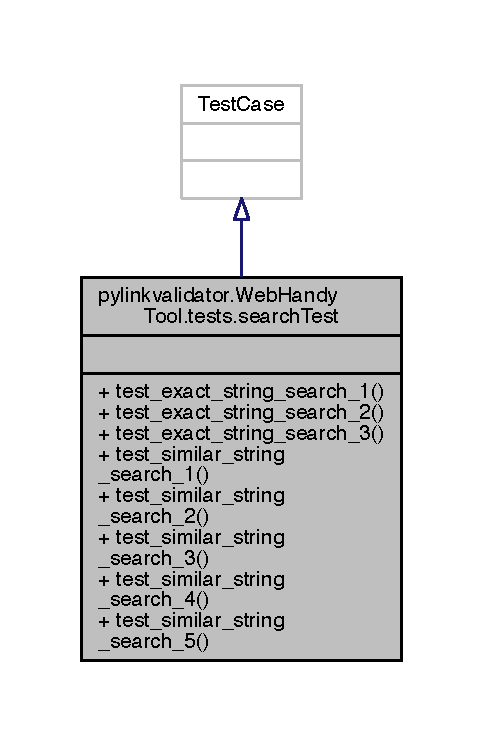
\includegraphics[width=232pt]{classpylinkvalidator_1_1_web_handy_tool_1_1tests_1_1search_test__inherit__graph}
\end{center}
\end{figure}


Collaboration diagram for pylinkvalidator.\+Web\+Handy\+Tool.\+tests.\+search\+Test\+:
\nopagebreak
\begin{figure}[H]
\begin{center}
\leavevmode
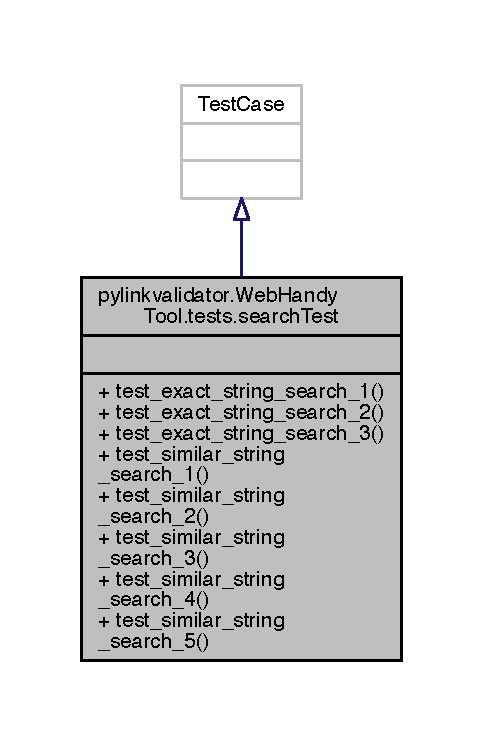
\includegraphics[width=232pt]{classpylinkvalidator_1_1_web_handy_tool_1_1tests_1_1search_test__coll__graph}
\end{center}
\end{figure}
\subsection*{Public Member Functions}
\begin{DoxyCompactItemize}
\item 
def \hyperlink{classpylinkvalidator_1_1_web_handy_tool_1_1tests_1_1search_test_a22af068c76d651d26ddec1e3570a6940}{test\+\_\+exact\+\_\+string\+\_\+search\+\_\+1} (self)
\item 
def \hyperlink{classpylinkvalidator_1_1_web_handy_tool_1_1tests_1_1search_test_a6a143b588cd317e507c1036eb1cff74c}{test\+\_\+exact\+\_\+string\+\_\+search\+\_\+2} (self)
\item 
def \hyperlink{classpylinkvalidator_1_1_web_handy_tool_1_1tests_1_1search_test_a812392a789426a4dfcaf6426969926a2}{test\+\_\+exact\+\_\+string\+\_\+search\+\_\+3} (self)
\item 
def \hyperlink{classpylinkvalidator_1_1_web_handy_tool_1_1tests_1_1search_test_add0a85705a03e79c4f5cce6d3e561970}{test\+\_\+similar\+\_\+string\+\_\+search\+\_\+1} (self)
\item 
def \hyperlink{classpylinkvalidator_1_1_web_handy_tool_1_1tests_1_1search_test_acd6db92558eb31dd8056ae2f78eb9a44}{test\+\_\+similar\+\_\+string\+\_\+search\+\_\+2} (self)
\item 
def \hyperlink{classpylinkvalidator_1_1_web_handy_tool_1_1tests_1_1search_test_af29247a2451b8eb1bba4128d11894623}{test\+\_\+similar\+\_\+string\+\_\+search\+\_\+3} (self)
\item 
def \hyperlink{classpylinkvalidator_1_1_web_handy_tool_1_1tests_1_1search_test_a4b8eb65b213a20cc9ffb5cceee0d3edd}{test\+\_\+similar\+\_\+string\+\_\+search\+\_\+4} (self)
\item 
def \hyperlink{classpylinkvalidator_1_1_web_handy_tool_1_1tests_1_1search_test_af1b354dddca2b2e216ce2961126b69c4}{test\+\_\+similar\+\_\+string\+\_\+search\+\_\+5} (self)
\end{DoxyCompactItemize}


\subsection{Member Function Documentation}
\index{pylinkvalidator\+::\+Web\+Handy\+Tool\+::tests\+::search\+Test@{pylinkvalidator\+::\+Web\+Handy\+Tool\+::tests\+::search\+Test}!test\+\_\+exact\+\_\+string\+\_\+search\+\_\+1@{test\+\_\+exact\+\_\+string\+\_\+search\+\_\+1}}
\index{test\+\_\+exact\+\_\+string\+\_\+search\+\_\+1@{test\+\_\+exact\+\_\+string\+\_\+search\+\_\+1}!pylinkvalidator\+::\+Web\+Handy\+Tool\+::tests\+::search\+Test@{pylinkvalidator\+::\+Web\+Handy\+Tool\+::tests\+::search\+Test}}
\subsubsection[{test\+\_\+exact\+\_\+string\+\_\+search\+\_\+1(self)}]{\setlength{\rightskip}{0pt plus 5cm}def pylinkvalidator.\+Web\+Handy\+Tool.\+tests.\+search\+Test.\+test\+\_\+exact\+\_\+string\+\_\+search\+\_\+1 (
\begin{DoxyParamCaption}
\item[{}]{self}
\end{DoxyParamCaption}
)}\hypertarget{classpylinkvalidator_1_1_web_handy_tool_1_1tests_1_1search_test_a22af068c76d651d26ddec1e3570a6940}{}\label{classpylinkvalidator_1_1_web_handy_tool_1_1tests_1_1search_test_a22af068c76d651d26ddec1e3570a6940}
\index{pylinkvalidator\+::\+Web\+Handy\+Tool\+::tests\+::search\+Test@{pylinkvalidator\+::\+Web\+Handy\+Tool\+::tests\+::search\+Test}!test\+\_\+exact\+\_\+string\+\_\+search\+\_\+2@{test\+\_\+exact\+\_\+string\+\_\+search\+\_\+2}}
\index{test\+\_\+exact\+\_\+string\+\_\+search\+\_\+2@{test\+\_\+exact\+\_\+string\+\_\+search\+\_\+2}!pylinkvalidator\+::\+Web\+Handy\+Tool\+::tests\+::search\+Test@{pylinkvalidator\+::\+Web\+Handy\+Tool\+::tests\+::search\+Test}}
\subsubsection[{test\+\_\+exact\+\_\+string\+\_\+search\+\_\+2(self)}]{\setlength{\rightskip}{0pt plus 5cm}def pylinkvalidator.\+Web\+Handy\+Tool.\+tests.\+search\+Test.\+test\+\_\+exact\+\_\+string\+\_\+search\+\_\+2 (
\begin{DoxyParamCaption}
\item[{}]{self}
\end{DoxyParamCaption}
)}\hypertarget{classpylinkvalidator_1_1_web_handy_tool_1_1tests_1_1search_test_a6a143b588cd317e507c1036eb1cff74c}{}\label{classpylinkvalidator_1_1_web_handy_tool_1_1tests_1_1search_test_a6a143b588cd317e507c1036eb1cff74c}
\index{pylinkvalidator\+::\+Web\+Handy\+Tool\+::tests\+::search\+Test@{pylinkvalidator\+::\+Web\+Handy\+Tool\+::tests\+::search\+Test}!test\+\_\+exact\+\_\+string\+\_\+search\+\_\+3@{test\+\_\+exact\+\_\+string\+\_\+search\+\_\+3}}
\index{test\+\_\+exact\+\_\+string\+\_\+search\+\_\+3@{test\+\_\+exact\+\_\+string\+\_\+search\+\_\+3}!pylinkvalidator\+::\+Web\+Handy\+Tool\+::tests\+::search\+Test@{pylinkvalidator\+::\+Web\+Handy\+Tool\+::tests\+::search\+Test}}
\subsubsection[{test\+\_\+exact\+\_\+string\+\_\+search\+\_\+3(self)}]{\setlength{\rightskip}{0pt plus 5cm}def pylinkvalidator.\+Web\+Handy\+Tool.\+tests.\+search\+Test.\+test\+\_\+exact\+\_\+string\+\_\+search\+\_\+3 (
\begin{DoxyParamCaption}
\item[{}]{self}
\end{DoxyParamCaption}
)}\hypertarget{classpylinkvalidator_1_1_web_handy_tool_1_1tests_1_1search_test_a812392a789426a4dfcaf6426969926a2}{}\label{classpylinkvalidator_1_1_web_handy_tool_1_1tests_1_1search_test_a812392a789426a4dfcaf6426969926a2}
\index{pylinkvalidator\+::\+Web\+Handy\+Tool\+::tests\+::search\+Test@{pylinkvalidator\+::\+Web\+Handy\+Tool\+::tests\+::search\+Test}!test\+\_\+similar\+\_\+string\+\_\+search\+\_\+1@{test\+\_\+similar\+\_\+string\+\_\+search\+\_\+1}}
\index{test\+\_\+similar\+\_\+string\+\_\+search\+\_\+1@{test\+\_\+similar\+\_\+string\+\_\+search\+\_\+1}!pylinkvalidator\+::\+Web\+Handy\+Tool\+::tests\+::search\+Test@{pylinkvalidator\+::\+Web\+Handy\+Tool\+::tests\+::search\+Test}}
\subsubsection[{test\+\_\+similar\+\_\+string\+\_\+search\+\_\+1(self)}]{\setlength{\rightskip}{0pt plus 5cm}def pylinkvalidator.\+Web\+Handy\+Tool.\+tests.\+search\+Test.\+test\+\_\+similar\+\_\+string\+\_\+search\+\_\+1 (
\begin{DoxyParamCaption}
\item[{}]{self}
\end{DoxyParamCaption}
)}\hypertarget{classpylinkvalidator_1_1_web_handy_tool_1_1tests_1_1search_test_add0a85705a03e79c4f5cce6d3e561970}{}\label{classpylinkvalidator_1_1_web_handy_tool_1_1tests_1_1search_test_add0a85705a03e79c4f5cce6d3e561970}
\index{pylinkvalidator\+::\+Web\+Handy\+Tool\+::tests\+::search\+Test@{pylinkvalidator\+::\+Web\+Handy\+Tool\+::tests\+::search\+Test}!test\+\_\+similar\+\_\+string\+\_\+search\+\_\+2@{test\+\_\+similar\+\_\+string\+\_\+search\+\_\+2}}
\index{test\+\_\+similar\+\_\+string\+\_\+search\+\_\+2@{test\+\_\+similar\+\_\+string\+\_\+search\+\_\+2}!pylinkvalidator\+::\+Web\+Handy\+Tool\+::tests\+::search\+Test@{pylinkvalidator\+::\+Web\+Handy\+Tool\+::tests\+::search\+Test}}
\subsubsection[{test\+\_\+similar\+\_\+string\+\_\+search\+\_\+2(self)}]{\setlength{\rightskip}{0pt plus 5cm}def pylinkvalidator.\+Web\+Handy\+Tool.\+tests.\+search\+Test.\+test\+\_\+similar\+\_\+string\+\_\+search\+\_\+2 (
\begin{DoxyParamCaption}
\item[{}]{self}
\end{DoxyParamCaption}
)}\hypertarget{classpylinkvalidator_1_1_web_handy_tool_1_1tests_1_1search_test_acd6db92558eb31dd8056ae2f78eb9a44}{}\label{classpylinkvalidator_1_1_web_handy_tool_1_1tests_1_1search_test_acd6db92558eb31dd8056ae2f78eb9a44}
\index{pylinkvalidator\+::\+Web\+Handy\+Tool\+::tests\+::search\+Test@{pylinkvalidator\+::\+Web\+Handy\+Tool\+::tests\+::search\+Test}!test\+\_\+similar\+\_\+string\+\_\+search\+\_\+3@{test\+\_\+similar\+\_\+string\+\_\+search\+\_\+3}}
\index{test\+\_\+similar\+\_\+string\+\_\+search\+\_\+3@{test\+\_\+similar\+\_\+string\+\_\+search\+\_\+3}!pylinkvalidator\+::\+Web\+Handy\+Tool\+::tests\+::search\+Test@{pylinkvalidator\+::\+Web\+Handy\+Tool\+::tests\+::search\+Test}}
\subsubsection[{test\+\_\+similar\+\_\+string\+\_\+search\+\_\+3(self)}]{\setlength{\rightskip}{0pt plus 5cm}def pylinkvalidator.\+Web\+Handy\+Tool.\+tests.\+search\+Test.\+test\+\_\+similar\+\_\+string\+\_\+search\+\_\+3 (
\begin{DoxyParamCaption}
\item[{}]{self}
\end{DoxyParamCaption}
)}\hypertarget{classpylinkvalidator_1_1_web_handy_tool_1_1tests_1_1search_test_af29247a2451b8eb1bba4128d11894623}{}\label{classpylinkvalidator_1_1_web_handy_tool_1_1tests_1_1search_test_af29247a2451b8eb1bba4128d11894623}
\index{pylinkvalidator\+::\+Web\+Handy\+Tool\+::tests\+::search\+Test@{pylinkvalidator\+::\+Web\+Handy\+Tool\+::tests\+::search\+Test}!test\+\_\+similar\+\_\+string\+\_\+search\+\_\+4@{test\+\_\+similar\+\_\+string\+\_\+search\+\_\+4}}
\index{test\+\_\+similar\+\_\+string\+\_\+search\+\_\+4@{test\+\_\+similar\+\_\+string\+\_\+search\+\_\+4}!pylinkvalidator\+::\+Web\+Handy\+Tool\+::tests\+::search\+Test@{pylinkvalidator\+::\+Web\+Handy\+Tool\+::tests\+::search\+Test}}
\subsubsection[{test\+\_\+similar\+\_\+string\+\_\+search\+\_\+4(self)}]{\setlength{\rightskip}{0pt plus 5cm}def pylinkvalidator.\+Web\+Handy\+Tool.\+tests.\+search\+Test.\+test\+\_\+similar\+\_\+string\+\_\+search\+\_\+4 (
\begin{DoxyParamCaption}
\item[{}]{self}
\end{DoxyParamCaption}
)}\hypertarget{classpylinkvalidator_1_1_web_handy_tool_1_1tests_1_1search_test_a4b8eb65b213a20cc9ffb5cceee0d3edd}{}\label{classpylinkvalidator_1_1_web_handy_tool_1_1tests_1_1search_test_a4b8eb65b213a20cc9ffb5cceee0d3edd}
\index{pylinkvalidator\+::\+Web\+Handy\+Tool\+::tests\+::search\+Test@{pylinkvalidator\+::\+Web\+Handy\+Tool\+::tests\+::search\+Test}!test\+\_\+similar\+\_\+string\+\_\+search\+\_\+5@{test\+\_\+similar\+\_\+string\+\_\+search\+\_\+5}}
\index{test\+\_\+similar\+\_\+string\+\_\+search\+\_\+5@{test\+\_\+similar\+\_\+string\+\_\+search\+\_\+5}!pylinkvalidator\+::\+Web\+Handy\+Tool\+::tests\+::search\+Test@{pylinkvalidator\+::\+Web\+Handy\+Tool\+::tests\+::search\+Test}}
\subsubsection[{test\+\_\+similar\+\_\+string\+\_\+search\+\_\+5(self)}]{\setlength{\rightskip}{0pt plus 5cm}def pylinkvalidator.\+Web\+Handy\+Tool.\+tests.\+search\+Test.\+test\+\_\+similar\+\_\+string\+\_\+search\+\_\+5 (
\begin{DoxyParamCaption}
\item[{}]{self}
\end{DoxyParamCaption}
)}\hypertarget{classpylinkvalidator_1_1_web_handy_tool_1_1tests_1_1search_test_af1b354dddca2b2e216ce2961126b69c4}{}\label{classpylinkvalidator_1_1_web_handy_tool_1_1tests_1_1search_test_af1b354dddca2b2e216ce2961126b69c4}


The documentation for this class was generated from the following file\+:\begin{DoxyCompactItemize}
\item 
Web\+Handy\+Tool/\hyperlink{tests_8py}{tests.\+py}\end{DoxyCompactItemize}

\hypertarget{class_test_string_1_1_test_string_methods}{}\section{Test\+String.\+Test\+String\+Methods Class Reference}
\label{class_test_string_1_1_test_string_methods}\index{Test\+String.\+Test\+String\+Methods@{Test\+String.\+Test\+String\+Methods}}


Inheritance diagram for Test\+String.\+Test\+String\+Methods\+:
\nopagebreak
\begin{figure}[H]
\begin{center}
\leavevmode
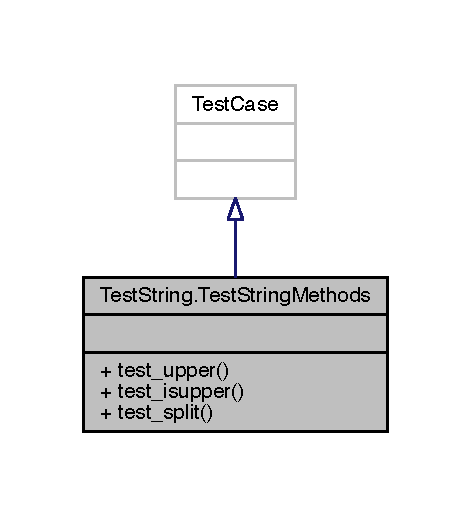
\includegraphics[width=226pt]{class_test_string_1_1_test_string_methods__inherit__graph}
\end{center}
\end{figure}


Collaboration diagram for Test\+String.\+Test\+String\+Methods\+:
\nopagebreak
\begin{figure}[H]
\begin{center}
\leavevmode
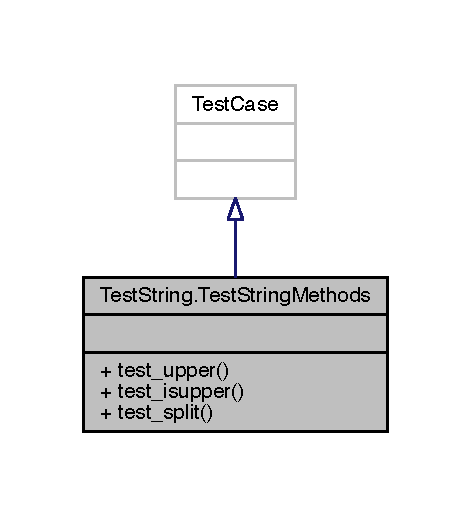
\includegraphics[width=226pt]{class_test_string_1_1_test_string_methods__coll__graph}
\end{center}
\end{figure}
\subsection*{Public Member Functions}
\begin{DoxyCompactItemize}
\item 
def {\bfseries test\+\_\+upper} (self)\hypertarget{class_test_string_1_1_test_string_methods_abd3a37be3b26c3bf46c303db0c03b7e5}{}\label{class_test_string_1_1_test_string_methods_abd3a37be3b26c3bf46c303db0c03b7e5}

\item 
def {\bfseries test\+\_\+isupper} (self)\hypertarget{class_test_string_1_1_test_string_methods_a6529ba420211e4577fa0c79ab7b20e1a}{}\label{class_test_string_1_1_test_string_methods_a6529ba420211e4577fa0c79ab7b20e1a}

\item 
def {\bfseries test\+\_\+split} (self)\hypertarget{class_test_string_1_1_test_string_methods_a3e28d67b465886b07c81361541ce839f}{}\label{class_test_string_1_1_test_string_methods_a3e28d67b465886b07c81361541ce839f}

\end{DoxyCompactItemize}


The documentation for this class was generated from the following file\+:\begin{DoxyCompactItemize}
\item 
files\+Just\+For\+Submission/Test\+String.\+py\end{DoxyCompactItemize}

\hypertarget{classpylinkvalidator_1_1_web_handy_tool_1_1tests_1_1_threaded_t_c_p_server}{}\section{pylinkvalidator.\+Web\+Handy\+Tool.\+tests.\+Threaded\+T\+C\+P\+Server Class Reference}
\label{classpylinkvalidator_1_1_web_handy_tool_1_1tests_1_1_threaded_t_c_p_server}\index{pylinkvalidator.\+Web\+Handy\+Tool.\+tests.\+Threaded\+T\+C\+P\+Server@{pylinkvalidator.\+Web\+Handy\+Tool.\+tests.\+Threaded\+T\+C\+P\+Server}}


Inheritance diagram for pylinkvalidator.\+Web\+Handy\+Tool.\+tests.\+Threaded\+T\+C\+P\+Server\+:
\nopagebreak
\begin{figure}[H]
\begin{center}
\leavevmode
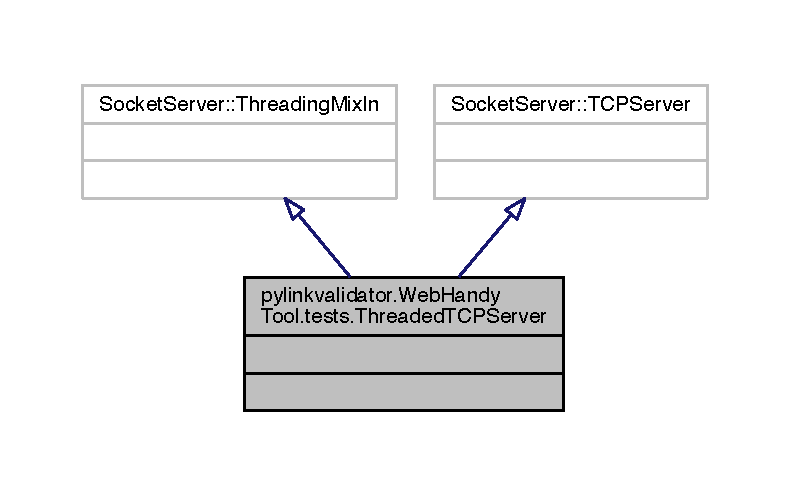
\includegraphics[width=350pt]{classpylinkvalidator_1_1_web_handy_tool_1_1tests_1_1_threaded_t_c_p_server__inherit__graph}
\end{center}
\end{figure}


Collaboration diagram for pylinkvalidator.\+Web\+Handy\+Tool.\+tests.\+Threaded\+T\+C\+P\+Server\+:
\nopagebreak
\begin{figure}[H]
\begin{center}
\leavevmode
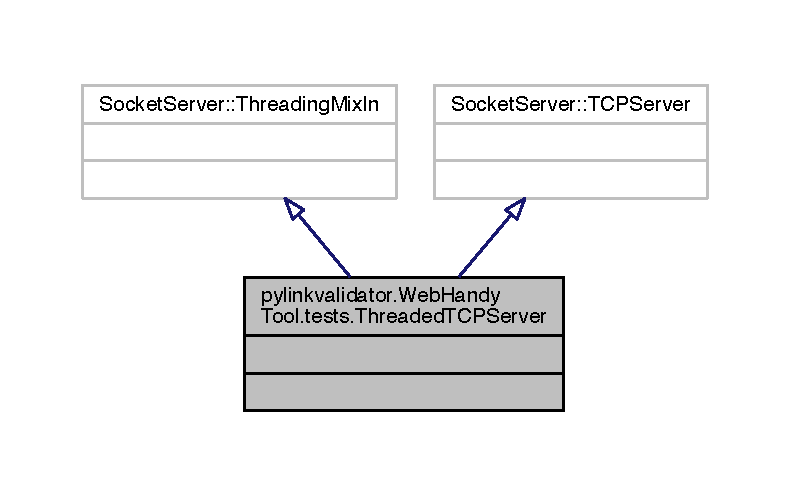
\includegraphics[width=350pt]{classpylinkvalidator_1_1_web_handy_tool_1_1tests_1_1_threaded_t_c_p_server__coll__graph}
\end{center}
\end{figure}


The documentation for this class was generated from the following file\+:\begin{DoxyCompactItemize}
\item 
Web\+Handy\+Tool/\hyperlink{tests_8py}{tests.\+py}\end{DoxyCompactItemize}

\hypertarget{classpylinkvalidator_1_1_web_handy_tool_1_1url_corrector_1_1url_corrector}{}\section{pylinkvalidator.\+Web\+Handy\+Tool.\+url\+Corrector.\+url\+Corrector Class Reference}
\label{classpylinkvalidator_1_1_web_handy_tool_1_1url_corrector_1_1url_corrector}\index{pylinkvalidator.\+Web\+Handy\+Tool.\+url\+Corrector.\+url\+Corrector@{pylinkvalidator.\+Web\+Handy\+Tool.\+url\+Corrector.\+url\+Corrector}}


Inheritance diagram for pylinkvalidator.\+Web\+Handy\+Tool.\+url\+Corrector.\+url\+Corrector\+:
\nopagebreak
\begin{figure}[H]
\begin{center}
\leavevmode
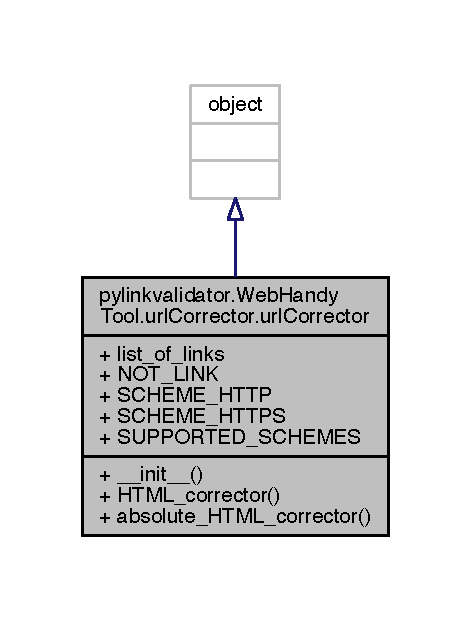
\includegraphics[width=226pt]{classpylinkvalidator_1_1_web_handy_tool_1_1url_corrector_1_1url_corrector__inherit__graph}
\end{center}
\end{figure}


Collaboration diagram for pylinkvalidator.\+Web\+Handy\+Tool.\+url\+Corrector.\+url\+Corrector\+:
\nopagebreak
\begin{figure}[H]
\begin{center}
\leavevmode
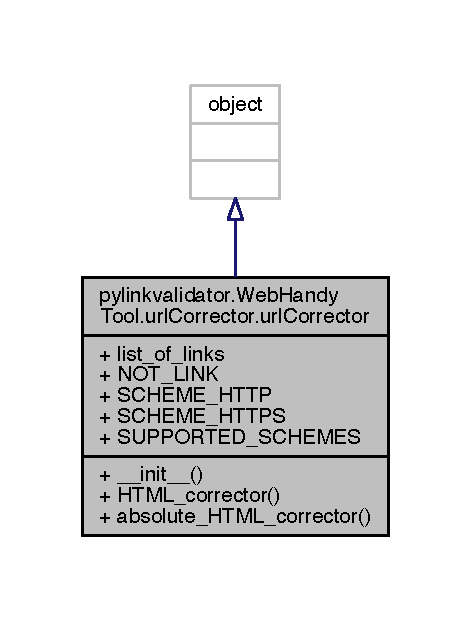
\includegraphics[width=226pt]{classpylinkvalidator_1_1_web_handy_tool_1_1url_corrector_1_1url_corrector__coll__graph}
\end{center}
\end{figure}
\subsection*{Public Member Functions}
\begin{DoxyCompactItemize}
\item 
def \hyperlink{classpylinkvalidator_1_1_web_handy_tool_1_1url_corrector_1_1url_corrector_a74c7cfee65534308bc6ed2ff2731d87a}{\+\_\+\+\_\+init\+\_\+\+\_\+} (self)
\item 
def \hyperlink{classpylinkvalidator_1_1_web_handy_tool_1_1url_corrector_1_1url_corrector_a5779046db561bf9a2716aa3189af838b}{H\+T\+M\+L\+\_\+corrector} (self, link)
\item 
def \hyperlink{classpylinkvalidator_1_1_web_handy_tool_1_1url_corrector_1_1url_corrector_a4c652295a197e0cb7a967628c627d441}{absolute\+\_\+\+H\+T\+M\+L\+\_\+corrector} (self, link, base\+\_\+link\+\_\+split)
\end{DoxyCompactItemize}
\subsection*{Public Attributes}
\begin{DoxyCompactItemize}
\item 
\hyperlink{classpylinkvalidator_1_1_web_handy_tool_1_1url_corrector_1_1url_corrector_aa94922a0d69691e5a1a06cd15965bb4c}{list\+\_\+of\+\_\+links}
\item 
\hyperlink{classpylinkvalidator_1_1_web_handy_tool_1_1url_corrector_1_1url_corrector_a7aa527e3b15ca61414c7fafcf07c26f7}{N\+O\+T\+\_\+\+L\+I\+NK}
\item 
\hyperlink{classpylinkvalidator_1_1_web_handy_tool_1_1url_corrector_1_1url_corrector_a2106176e98a66feeef4b49729caebb94}{S\+C\+H\+E\+M\+E\+\_\+\+H\+T\+TP}
\item 
\hyperlink{classpylinkvalidator_1_1_web_handy_tool_1_1url_corrector_1_1url_corrector_af2a52a31f8cb0410112f845ddf8f75d5}{S\+C\+H\+E\+M\+E\+\_\+\+H\+T\+T\+PS}
\item 
\hyperlink{classpylinkvalidator_1_1_web_handy_tool_1_1url_corrector_1_1url_corrector_ab43ea2d3a9244b23ce58ea5e63934d1b}{S\+U\+P\+P\+O\+R\+T\+E\+D\+\_\+\+S\+C\+H\+E\+M\+ES}
\end{DoxyCompactItemize}


\subsection{Constructor \& Destructor Documentation}
\index{pylinkvalidator\+::\+Web\+Handy\+Tool\+::url\+Corrector\+::url\+Corrector@{pylinkvalidator\+::\+Web\+Handy\+Tool\+::url\+Corrector\+::url\+Corrector}!\+\_\+\+\_\+init\+\_\+\+\_\+@{\+\_\+\+\_\+init\+\_\+\+\_\+}}
\index{\+\_\+\+\_\+init\+\_\+\+\_\+@{\+\_\+\+\_\+init\+\_\+\+\_\+}!pylinkvalidator\+::\+Web\+Handy\+Tool\+::url\+Corrector\+::url\+Corrector@{pylinkvalidator\+::\+Web\+Handy\+Tool\+::url\+Corrector\+::url\+Corrector}}
\subsubsection[{\+\_\+\+\_\+init\+\_\+\+\_\+(self)}]{\setlength{\rightskip}{0pt plus 5cm}def pylinkvalidator.\+Web\+Handy\+Tool.\+url\+Corrector.\+url\+Corrector.\+\_\+\+\_\+init\+\_\+\+\_\+ (
\begin{DoxyParamCaption}
\item[{}]{self}
\end{DoxyParamCaption}
)}\hypertarget{classpylinkvalidator_1_1_web_handy_tool_1_1url_corrector_1_1url_corrector_a74c7cfee65534308bc6ed2ff2731d87a}{}\label{classpylinkvalidator_1_1_web_handy_tool_1_1url_corrector_1_1url_corrector_a74c7cfee65534308bc6ed2ff2731d87a}


\subsection{Member Function Documentation}
\index{pylinkvalidator\+::\+Web\+Handy\+Tool\+::url\+Corrector\+::url\+Corrector@{pylinkvalidator\+::\+Web\+Handy\+Tool\+::url\+Corrector\+::url\+Corrector}!absolute\+\_\+\+H\+T\+M\+L\+\_\+corrector@{absolute\+\_\+\+H\+T\+M\+L\+\_\+corrector}}
\index{absolute\+\_\+\+H\+T\+M\+L\+\_\+corrector@{absolute\+\_\+\+H\+T\+M\+L\+\_\+corrector}!pylinkvalidator\+::\+Web\+Handy\+Tool\+::url\+Corrector\+::url\+Corrector@{pylinkvalidator\+::\+Web\+Handy\+Tool\+::url\+Corrector\+::url\+Corrector}}
\subsubsection[{absolute\+\_\+\+H\+T\+M\+L\+\_\+corrector(self, link, base\+\_\+link\+\_\+split)}]{\setlength{\rightskip}{0pt plus 5cm}def pylinkvalidator.\+Web\+Handy\+Tool.\+url\+Corrector.\+url\+Corrector.\+absolute\+\_\+\+H\+T\+M\+L\+\_\+corrector (
\begin{DoxyParamCaption}
\item[{}]{self, }
\item[{}]{link, }
\item[{}]{base\+\_\+link\+\_\+split}
\end{DoxyParamCaption}
)}\hypertarget{classpylinkvalidator_1_1_web_handy_tool_1_1url_corrector_1_1url_corrector_a4c652295a197e0cb7a967628c627d441}{}\label{classpylinkvalidator_1_1_web_handy_tool_1_1url_corrector_1_1url_corrector_a4c652295a197e0cb7a967628c627d441}
\begin{DoxyVerb}Takes in the base url and appends any relative or absolute links to the base urk.

:param link:
:param base_link_split:
:return Url object of split url result corrected link Ex; SplitResult(scheme=u'http', netloc=u'canvasgroup.ca', path=u'/zdfzd', query=u'', fragment=u'') ::
\end{DoxyVerb}
 

Here is the call graph for this function\+:
\nopagebreak
\begin{figure}[H]
\begin{center}
\leavevmode
\includegraphics[width=350pt]{classpylinkvalidator_1_1_web_handy_tool_1_1url_corrector_1_1url_corrector_a4c652295a197e0cb7a967628c627d441_cgraph}
\end{center}
\end{figure}


\index{pylinkvalidator\+::\+Web\+Handy\+Tool\+::url\+Corrector\+::url\+Corrector@{pylinkvalidator\+::\+Web\+Handy\+Tool\+::url\+Corrector\+::url\+Corrector}!H\+T\+M\+L\+\_\+corrector@{H\+T\+M\+L\+\_\+corrector}}
\index{H\+T\+M\+L\+\_\+corrector@{H\+T\+M\+L\+\_\+corrector}!pylinkvalidator\+::\+Web\+Handy\+Tool\+::url\+Corrector\+::url\+Corrector@{pylinkvalidator\+::\+Web\+Handy\+Tool\+::url\+Corrector\+::url\+Corrector}}
\subsubsection[{H\+T\+M\+L\+\_\+corrector(self, link)}]{\setlength{\rightskip}{0pt plus 5cm}def pylinkvalidator.\+Web\+Handy\+Tool.\+url\+Corrector.\+url\+Corrector.\+H\+T\+M\+L\+\_\+corrector (
\begin{DoxyParamCaption}
\item[{}]{self, }
\item[{}]{link}
\end{DoxyParamCaption}
)}\hypertarget{classpylinkvalidator_1_1_web_handy_tool_1_1url_corrector_1_1url_corrector_a5779046db561bf9a2716aa3189af838b}{}\label{classpylinkvalidator_1_1_web_handy_tool_1_1url_corrector_1_1url_corrector_a5779046db561bf9a2716aa3189af838b}
\begin{DoxyVerb}Fixes the link passed in such that it becomes either a functioning link or is flagged as a broken link.
:param link:
:return  Url object of split url result corrected link Ex; SplitResult(scheme=u'http', netloc=u'canvasgroup.ca', path=u'/zdfzd', query=u'', fragment=u'') :
\end{DoxyVerb}
 

Here is the caller graph for this function\+:
\nopagebreak
\begin{figure}[H]
\begin{center}
\leavevmode
\includegraphics[width=350pt]{classpylinkvalidator_1_1_web_handy_tool_1_1url_corrector_1_1url_corrector_a5779046db561bf9a2716aa3189af838b_icgraph}
\end{center}
\end{figure}




\subsection{Member Data Documentation}
\index{pylinkvalidator\+::\+Web\+Handy\+Tool\+::url\+Corrector\+::url\+Corrector@{pylinkvalidator\+::\+Web\+Handy\+Tool\+::url\+Corrector\+::url\+Corrector}!list\+\_\+of\+\_\+links@{list\+\_\+of\+\_\+links}}
\index{list\+\_\+of\+\_\+links@{list\+\_\+of\+\_\+links}!pylinkvalidator\+::\+Web\+Handy\+Tool\+::url\+Corrector\+::url\+Corrector@{pylinkvalidator\+::\+Web\+Handy\+Tool\+::url\+Corrector\+::url\+Corrector}}
\subsubsection[{list\+\_\+of\+\_\+links}]{\setlength{\rightskip}{0pt plus 5cm}pylinkvalidator.\+Web\+Handy\+Tool.\+url\+Corrector.\+url\+Corrector.\+list\+\_\+of\+\_\+links}\hypertarget{classpylinkvalidator_1_1_web_handy_tool_1_1url_corrector_1_1url_corrector_aa94922a0d69691e5a1a06cd15965bb4c}{}\label{classpylinkvalidator_1_1_web_handy_tool_1_1url_corrector_1_1url_corrector_aa94922a0d69691e5a1a06cd15965bb4c}
\index{pylinkvalidator\+::\+Web\+Handy\+Tool\+::url\+Corrector\+::url\+Corrector@{pylinkvalidator\+::\+Web\+Handy\+Tool\+::url\+Corrector\+::url\+Corrector}!N\+O\+T\+\_\+\+L\+I\+NK@{N\+O\+T\+\_\+\+L\+I\+NK}}
\index{N\+O\+T\+\_\+\+L\+I\+NK@{N\+O\+T\+\_\+\+L\+I\+NK}!pylinkvalidator\+::\+Web\+Handy\+Tool\+::url\+Corrector\+::url\+Corrector@{pylinkvalidator\+::\+Web\+Handy\+Tool\+::url\+Corrector\+::url\+Corrector}}
\subsubsection[{N\+O\+T\+\_\+\+L\+I\+NK}]{\setlength{\rightskip}{0pt plus 5cm}pylinkvalidator.\+Web\+Handy\+Tool.\+url\+Corrector.\+url\+Corrector.\+N\+O\+T\+\_\+\+L\+I\+NK}\hypertarget{classpylinkvalidator_1_1_web_handy_tool_1_1url_corrector_1_1url_corrector_a7aa527e3b15ca61414c7fafcf07c26f7}{}\label{classpylinkvalidator_1_1_web_handy_tool_1_1url_corrector_1_1url_corrector_a7aa527e3b15ca61414c7fafcf07c26f7}
\index{pylinkvalidator\+::\+Web\+Handy\+Tool\+::url\+Corrector\+::url\+Corrector@{pylinkvalidator\+::\+Web\+Handy\+Tool\+::url\+Corrector\+::url\+Corrector}!S\+C\+H\+E\+M\+E\+\_\+\+H\+T\+TP@{S\+C\+H\+E\+M\+E\+\_\+\+H\+T\+TP}}
\index{S\+C\+H\+E\+M\+E\+\_\+\+H\+T\+TP@{S\+C\+H\+E\+M\+E\+\_\+\+H\+T\+TP}!pylinkvalidator\+::\+Web\+Handy\+Tool\+::url\+Corrector\+::url\+Corrector@{pylinkvalidator\+::\+Web\+Handy\+Tool\+::url\+Corrector\+::url\+Corrector}}
\subsubsection[{S\+C\+H\+E\+M\+E\+\_\+\+H\+T\+TP}]{\setlength{\rightskip}{0pt plus 5cm}pylinkvalidator.\+Web\+Handy\+Tool.\+url\+Corrector.\+url\+Corrector.\+S\+C\+H\+E\+M\+E\+\_\+\+H\+T\+TP}\hypertarget{classpylinkvalidator_1_1_web_handy_tool_1_1url_corrector_1_1url_corrector_a2106176e98a66feeef4b49729caebb94}{}\label{classpylinkvalidator_1_1_web_handy_tool_1_1url_corrector_1_1url_corrector_a2106176e98a66feeef4b49729caebb94}
\index{pylinkvalidator\+::\+Web\+Handy\+Tool\+::url\+Corrector\+::url\+Corrector@{pylinkvalidator\+::\+Web\+Handy\+Tool\+::url\+Corrector\+::url\+Corrector}!S\+C\+H\+E\+M\+E\+\_\+\+H\+T\+T\+PS@{S\+C\+H\+E\+M\+E\+\_\+\+H\+T\+T\+PS}}
\index{S\+C\+H\+E\+M\+E\+\_\+\+H\+T\+T\+PS@{S\+C\+H\+E\+M\+E\+\_\+\+H\+T\+T\+PS}!pylinkvalidator\+::\+Web\+Handy\+Tool\+::url\+Corrector\+::url\+Corrector@{pylinkvalidator\+::\+Web\+Handy\+Tool\+::url\+Corrector\+::url\+Corrector}}
\subsubsection[{S\+C\+H\+E\+M\+E\+\_\+\+H\+T\+T\+PS}]{\setlength{\rightskip}{0pt plus 5cm}pylinkvalidator.\+Web\+Handy\+Tool.\+url\+Corrector.\+url\+Corrector.\+S\+C\+H\+E\+M\+E\+\_\+\+H\+T\+T\+PS}\hypertarget{classpylinkvalidator_1_1_web_handy_tool_1_1url_corrector_1_1url_corrector_af2a52a31f8cb0410112f845ddf8f75d5}{}\label{classpylinkvalidator_1_1_web_handy_tool_1_1url_corrector_1_1url_corrector_af2a52a31f8cb0410112f845ddf8f75d5}
\index{pylinkvalidator\+::\+Web\+Handy\+Tool\+::url\+Corrector\+::url\+Corrector@{pylinkvalidator\+::\+Web\+Handy\+Tool\+::url\+Corrector\+::url\+Corrector}!S\+U\+P\+P\+O\+R\+T\+E\+D\+\_\+\+S\+C\+H\+E\+M\+ES@{S\+U\+P\+P\+O\+R\+T\+E\+D\+\_\+\+S\+C\+H\+E\+M\+ES}}
\index{S\+U\+P\+P\+O\+R\+T\+E\+D\+\_\+\+S\+C\+H\+E\+M\+ES@{S\+U\+P\+P\+O\+R\+T\+E\+D\+\_\+\+S\+C\+H\+E\+M\+ES}!pylinkvalidator\+::\+Web\+Handy\+Tool\+::url\+Corrector\+::url\+Corrector@{pylinkvalidator\+::\+Web\+Handy\+Tool\+::url\+Corrector\+::url\+Corrector}}
\subsubsection[{S\+U\+P\+P\+O\+R\+T\+E\+D\+\_\+\+S\+C\+H\+E\+M\+ES}]{\setlength{\rightskip}{0pt plus 5cm}pylinkvalidator.\+Web\+Handy\+Tool.\+url\+Corrector.\+url\+Corrector.\+S\+U\+P\+P\+O\+R\+T\+E\+D\+\_\+\+S\+C\+H\+E\+M\+ES}\hypertarget{classpylinkvalidator_1_1_web_handy_tool_1_1url_corrector_1_1url_corrector_ab43ea2d3a9244b23ce58ea5e63934d1b}{}\label{classpylinkvalidator_1_1_web_handy_tool_1_1url_corrector_1_1url_corrector_ab43ea2d3a9244b23ce58ea5e63934d1b}


The documentation for this class was generated from the following file\+:\begin{DoxyCompactItemize}
\item 
Web\+Handy\+Tool/\hyperlink{url_corrector_8py}{url\+Corrector.\+py}\end{DoxyCompactItemize}

\hypertarget{classpylinkvalidator_1_1_web_handy_tool_1_1tests_1_1url_corrector_test}{}\section{pylinkvalidator.\+Web\+Handy\+Tool.\+tests.\+url\+Corrector\+Test Class Reference}
\label{classpylinkvalidator_1_1_web_handy_tool_1_1tests_1_1url_corrector_test}\index{pylinkvalidator.\+Web\+Handy\+Tool.\+tests.\+url\+Corrector\+Test@{pylinkvalidator.\+Web\+Handy\+Tool.\+tests.\+url\+Corrector\+Test}}


Inheritance diagram for pylinkvalidator.\+Web\+Handy\+Tool.\+tests.\+url\+Corrector\+Test\+:
\nopagebreak
\begin{figure}[H]
\begin{center}
\leavevmode
\includegraphics[width=212pt]{classpylinkvalidator_1_1_web_handy_tool_1_1tests_1_1url_corrector_test__inherit__graph}
\end{center}
\end{figure}


Collaboration diagram for pylinkvalidator.\+Web\+Handy\+Tool.\+tests.\+url\+Corrector\+Test\+:
\nopagebreak
\begin{figure}[H]
\begin{center}
\leavevmode
\includegraphics[width=212pt]{classpylinkvalidator_1_1_web_handy_tool_1_1tests_1_1url_corrector_test__coll__graph}
\end{center}
\end{figure}
\subsection*{Public Member Functions}
\begin{DoxyCompactItemize}
\item 
def \hyperlink{classpylinkvalidator_1_1_web_handy_tool_1_1tests_1_1url_corrector_test_adbeab76343c14a02620ed4b8b6fbb4fe}{test\+\_\+clean\+\_\+url\+\_\+split} (self)
\item 
def \hyperlink{classpylinkvalidator_1_1_web_handy_tool_1_1tests_1_1url_corrector_test_a7e73d3cd877f27c3f473733a6ccd4773}{test\+\_\+get\+\_\+absolute\+\_\+url} (self)
\end{DoxyCompactItemize}


\subsection{Member Function Documentation}
\index{pylinkvalidator\+::\+Web\+Handy\+Tool\+::tests\+::url\+Corrector\+Test@{pylinkvalidator\+::\+Web\+Handy\+Tool\+::tests\+::url\+Corrector\+Test}!test\+\_\+clean\+\_\+url\+\_\+split@{test\+\_\+clean\+\_\+url\+\_\+split}}
\index{test\+\_\+clean\+\_\+url\+\_\+split@{test\+\_\+clean\+\_\+url\+\_\+split}!pylinkvalidator\+::\+Web\+Handy\+Tool\+::tests\+::url\+Corrector\+Test@{pylinkvalidator\+::\+Web\+Handy\+Tool\+::tests\+::url\+Corrector\+Test}}
\subsubsection[{test\+\_\+clean\+\_\+url\+\_\+split(self)}]{\setlength{\rightskip}{0pt plus 5cm}def pylinkvalidator.\+Web\+Handy\+Tool.\+tests.\+url\+Corrector\+Test.\+test\+\_\+clean\+\_\+url\+\_\+split (
\begin{DoxyParamCaption}
\item[{}]{self}
\end{DoxyParamCaption}
)}\hypertarget{classpylinkvalidator_1_1_web_handy_tool_1_1tests_1_1url_corrector_test_adbeab76343c14a02620ed4b8b6fbb4fe}{}\label{classpylinkvalidator_1_1_web_handy_tool_1_1tests_1_1url_corrector_test_adbeab76343c14a02620ed4b8b6fbb4fe}
\index{pylinkvalidator\+::\+Web\+Handy\+Tool\+::tests\+::url\+Corrector\+Test@{pylinkvalidator\+::\+Web\+Handy\+Tool\+::tests\+::url\+Corrector\+Test}!test\+\_\+get\+\_\+absolute\+\_\+url@{test\+\_\+get\+\_\+absolute\+\_\+url}}
\index{test\+\_\+get\+\_\+absolute\+\_\+url@{test\+\_\+get\+\_\+absolute\+\_\+url}!pylinkvalidator\+::\+Web\+Handy\+Tool\+::tests\+::url\+Corrector\+Test@{pylinkvalidator\+::\+Web\+Handy\+Tool\+::tests\+::url\+Corrector\+Test}}
\subsubsection[{test\+\_\+get\+\_\+absolute\+\_\+url(self)}]{\setlength{\rightskip}{0pt plus 5cm}def pylinkvalidator.\+Web\+Handy\+Tool.\+tests.\+url\+Corrector\+Test.\+test\+\_\+get\+\_\+absolute\+\_\+url (
\begin{DoxyParamCaption}
\item[{}]{self}
\end{DoxyParamCaption}
)}\hypertarget{classpylinkvalidator_1_1_web_handy_tool_1_1tests_1_1url_corrector_test_a7e73d3cd877f27c3f473733a6ccd4773}{}\label{classpylinkvalidator_1_1_web_handy_tool_1_1tests_1_1url_corrector_test_a7e73d3cd877f27c3f473733a6ccd4773}


The documentation for this class was generated from the following file\+:\begin{DoxyCompactItemize}
\item 
Web\+Handy\+Tool/\hyperlink{tests_8py}{tests.\+py}\end{DoxyCompactItemize}

\hypertarget{classpylinkvalidator_1_1_p_o_c_01_code_1_1_web___crawler_1_1_web___crawler}{}\section{pylinkvalidator.\+P\+OC Code.\+Web\+\_\+\+Crawler.\+Web\+\_\+\+Crawler Class Reference}
\label{classpylinkvalidator_1_1_p_o_c_01_code_1_1_web___crawler_1_1_web___crawler}\index{pylinkvalidator.\+P\+O\+C Code.\+Web\+\_\+\+Crawler.\+Web\+\_\+\+Crawler@{pylinkvalidator.\+P\+O\+C Code.\+Web\+\_\+\+Crawler.\+Web\+\_\+\+Crawler}}


Inheritance diagram for pylinkvalidator.\+P\+OC Code.\+Web\+\_\+\+Crawler.\+Web\+\_\+\+Crawler\+:
\nopagebreak
\begin{figure}[H]
\begin{center}
\leavevmode
\includegraphics[width=226pt]{classpylinkvalidator_1_1_p_o_c_01_code_1_1_web___crawler_1_1_web___crawler__inherit__graph}
\end{center}
\end{figure}


Collaboration diagram for pylinkvalidator.\+P\+OC Code.\+Web\+\_\+\+Crawler.\+Web\+\_\+\+Crawler\+:
\nopagebreak
\begin{figure}[H]
\begin{center}
\leavevmode
\includegraphics[width=226pt]{classpylinkvalidator_1_1_p_o_c_01_code_1_1_web___crawler_1_1_web___crawler__coll__graph}
\end{center}
\end{figure}
\subsection*{Public Member Functions}
\begin{DoxyCompactItemize}
\item 
def \hyperlink{classpylinkvalidator_1_1_p_o_c_01_code_1_1_web___crawler_1_1_web___crawler_a11f494a5019e83e4e97de9d02e70eac0}{\+\_\+\+\_\+init\+\_\+\+\_\+} (self)
\item 
def \hyperlink{classpylinkvalidator_1_1_p_o_c_01_code_1_1_web___crawler_1_1_web___crawler_ab88f99b20a665b945bbfbacd29c7cd35}{option} (self)
\item 
def \hyperlink{classpylinkvalidator_1_1_p_o_c_01_code_1_1_web___crawler_1_1_web___crawler_a56ce7ff8f340a4e3a12fa6af7aa685ef}{dfs} (self, \hyperlink{classpylinkvalidator_1_1_p_o_c_01_code_1_1_web___crawler_1_1_web___crawler_a4100bfbd077cd54c5ee1b6e3ad21ba05}{choice})
\item 
def \hyperlink{classpylinkvalidator_1_1_p_o_c_01_code_1_1_web___crawler_1_1_web___crawler_a5fc56f19ac8d7aa5a6f1dcc2dd2c7f43}{bfs} (self, link)
\item 
def \hyperlink{classpylinkvalidator_1_1_p_o_c_01_code_1_1_web___crawler_1_1_web___crawler_a685b38e7e243a8edbae39c1ee31ba866}{H\+T\+M\+L\+\_\+corrector} (self, link)
\item 
def \hyperlink{classpylinkvalidator_1_1_p_o_c_01_code_1_1_web___crawler_1_1_web___crawler_ac4ba57c891836fb48a2115d51538e9bc}{absolute\+\_\+\+H\+T\+M\+L\+\_\+corrector} (self, link, base\+\_\+link\+\_\+split)
\item 
def \hyperlink{classpylinkvalidator_1_1_p_o_c_01_code_1_1_web___crawler_1_1_web___crawler_a70b41cbe1f381fd211536be5b6ab6c49}{download\+\_\+resources} (self, link, options=\textquotesingle{}-\/rA\textquotesingle{}, file\+\_\+type=None)
\item 
def \hyperlink{classpylinkvalidator_1_1_p_o_c_01_code_1_1_web___crawler_1_1_web___crawler_afbaad82f02609f768b0c7fd9baa83048}{exact\+\_\+query} (self, query, data)
\item 
def \hyperlink{classpylinkvalidator_1_1_p_o_c_01_code_1_1_web___crawler_1_1_web___crawler_a0ac2dcc6a346b596678fd923ce62c422}{similar\+\_\+query} (self, query, data, proximity)
\item 
def \hyperlink{classpylinkvalidator_1_1_p_o_c_01_code_1_1_web___crawler_1_1_web___crawler_ad00325e9391b34decc4960520f929deb}{whitespace\+\_\+checker} (self, character)
\item 
def \hyperlink{classpylinkvalidator_1_1_p_o_c_01_code_1_1_web___crawler_1_1_web___crawler_a77d0c8f8dad271699c5c26a65c127767}{find\+\_\+links} (self, link, destination=None)
\item 
def \hyperlink{classpylinkvalidator_1_1_p_o_c_01_code_1_1_web___crawler_1_1_web___crawler_a2fc6c2e07ddf12c96da4216bc11763d5}{check\+\_\+errors} (self, link, \hyperlink{classpylinkvalidator_1_1_p_o_c_01_code_1_1_web___crawler_1_1_web___crawler_ac2956f25315755df07ef3ba47f283e83}{list\+\_\+of\+\_\+links}=None)
\item 
def \hyperlink{classpylinkvalidator_1_1_p_o_c_01_code_1_1_web___crawler_1_1_web___crawler_a09080daab7b16e68d2dbd4468079ae81}{B\+S\+\_\+parse\+\_\+data} (self, link)
\item 
def \hyperlink{classpylinkvalidator_1_1_p_o_c_01_code_1_1_web___crawler_1_1_web___crawler_a048a3be9f662196c8c355cb5f12c1cd8}{H\+T\+M\+L\+\_\+text} (self, link)
\item 
def \hyperlink{classpylinkvalidator_1_1_p_o_c_01_code_1_1_web___crawler_1_1_web___crawler_afac8f54efb9be45422268f8ccf9a5d48}{query\+\_\+search} (self, query, link, \hyperlink{classpylinkvalidator_1_1_p_o_c_01_code_1_1_web___crawler_1_1_web___crawler_ac2956f25315755df07ef3ba47f283e83}{list\+\_\+of\+\_\+links}=None, \hyperlink{classpylinkvalidator_1_1_p_o_c_01_code_1_1_web___crawler_1_1_web___crawler_a4100bfbd077cd54c5ee1b6e3ad21ba05}{choice}=\textquotesingle{}exact\textquotesingle{})
\item 
def \hyperlink{classpylinkvalidator_1_1_p_o_c_01_code_1_1_web___crawler_1_1_web___crawler_ac5547b7358459fc652278d1fd7306621}{depth\+\_\+setter} (self, \hyperlink{classpylinkvalidator_1_1_p_o_c_01_code_1_1_web___crawler_1_1_web___crawler_a4b25f5a1077981b4fc673a30cd6f60f5}{depth})
\item 
def \hyperlink{classpylinkvalidator_1_1_p_o_c_01_code_1_1_web___crawler_1_1_web___crawler_a0c6649825a52751d19cd23e093e2c6c3}{website\+\_\+\+Depth} (self, link, \hyperlink{classpylinkvalidator_1_1_p_o_c_01_code_1_1_web___crawler_1_1_web___crawler_a4b25f5a1077981b4fc673a30cd6f60f5}{depth})
\end{DoxyCompactItemize}
\subsection*{Public Attributes}
\begin{DoxyCompactItemize}
\item 
\hyperlink{classpylinkvalidator_1_1_p_o_c_01_code_1_1_web___crawler_1_1_web___crawler_a4b25f5a1077981b4fc673a30cd6f60f5}{depth}
\item 
\hyperlink{classpylinkvalidator_1_1_p_o_c_01_code_1_1_web___crawler_1_1_web___crawler_ae21f36bb8bac5b3a440e372a6898fdb3}{algo}
\item 
\hyperlink{classpylinkvalidator_1_1_p_o_c_01_code_1_1_web___crawler_1_1_web___crawler_a17e17d066349bf6795a8f3a6a2dfc909}{choices}
\item 
\hyperlink{classpylinkvalidator_1_1_p_o_c_01_code_1_1_web___crawler_1_1_web___crawler_a33c0a83d96930b31e2a8f0f81345a18f}{search\+\_\+choices}
\item 
\hyperlink{classpylinkvalidator_1_1_p_o_c_01_code_1_1_web___crawler_1_1_web___crawler_a4100bfbd077cd54c5ee1b6e3ad21ba05}{choice}
\item 
\hyperlink{classpylinkvalidator_1_1_p_o_c_01_code_1_1_web___crawler_1_1_web___crawler_ac2c45da364f56570078463b236a3db9a}{search\+\_\+choice}
\item 
\hyperlink{classpylinkvalidator_1_1_p_o_c_01_code_1_1_web___crawler_1_1_web___crawler_a72c07e1d106dac630b27ad7844742f21}{output}
\item 
\hyperlink{classpylinkvalidator_1_1_p_o_c_01_code_1_1_web___crawler_1_1_web___crawler_a783243f26a2aa6c636626231ec137c35}{seed}
\item 
\hyperlink{classpylinkvalidator_1_1_p_o_c_01_code_1_1_web___crawler_1_1_web___crawler_ac2956f25315755df07ef3ba47f283e83}{list\+\_\+of\+\_\+links}
\item 
\hyperlink{classpylinkvalidator_1_1_p_o_c_01_code_1_1_web___crawler_1_1_web___crawler_aad9d98c171e3d7014a3eee1d061e1381}{N\+O\+T\+\_\+\+L\+I\+NK}
\item 
\hyperlink{classpylinkvalidator_1_1_p_o_c_01_code_1_1_web___crawler_1_1_web___crawler_aa8af000696c151fe4972d098507e7654}{S\+C\+H\+E\+M\+E\+\_\+\+H\+T\+TP}
\item 
\hyperlink{classpylinkvalidator_1_1_p_o_c_01_code_1_1_web___crawler_1_1_web___crawler_a6d304fcbd84982b5b7560d9f7bd9f3d4}{S\+C\+H\+E\+M\+E\+\_\+\+H\+T\+T\+PS}
\item 
\hyperlink{classpylinkvalidator_1_1_p_o_c_01_code_1_1_web___crawler_1_1_web___crawler_a917f9b86adefbcb3dc0dc53075ebbd34}{S\+U\+P\+P\+O\+R\+T\+E\+D\+\_\+\+S\+C\+H\+E\+M\+ES}
\end{DoxyCompactItemize}


\subsection{Detailed Description}
\begin{DoxyVerb}Main class, it is for crawling.
Class variable includes depth,algo,choices,choice,output,seed,list of links
\end{DoxyVerb}
 

\subsection{Constructor \& Destructor Documentation}
\index{pylinkvalidator\+::\+P\+O\+C Code\+::\+Web\+\_\+\+Crawler\+::\+Web\+\_\+\+Crawler@{pylinkvalidator\+::\+P\+O\+C Code\+::\+Web\+\_\+\+Crawler\+::\+Web\+\_\+\+Crawler}!\+\_\+\+\_\+init\+\_\+\+\_\+@{\+\_\+\+\_\+init\+\_\+\+\_\+}}
\index{\+\_\+\+\_\+init\+\_\+\+\_\+@{\+\_\+\+\_\+init\+\_\+\+\_\+}!pylinkvalidator\+::\+P\+O\+C Code\+::\+Web\+\_\+\+Crawler\+::\+Web\+\_\+\+Crawler@{pylinkvalidator\+::\+P\+O\+C Code\+::\+Web\+\_\+\+Crawler\+::\+Web\+\_\+\+Crawler}}
\subsubsection[{\+\_\+\+\_\+init\+\_\+\+\_\+(self)}]{\setlength{\rightskip}{0pt plus 5cm}def pylinkvalidator.\+P\+OC Code.\+Web\+\_\+\+Crawler.\+Web\+\_\+\+Crawler.\+\_\+\+\_\+init\+\_\+\+\_\+ (
\begin{DoxyParamCaption}
\item[{}]{self}
\end{DoxyParamCaption}
)}\hypertarget{classpylinkvalidator_1_1_p_o_c_01_code_1_1_web___crawler_1_1_web___crawler_a11f494a5019e83e4e97de9d02e70eac0}{}\label{classpylinkvalidator_1_1_p_o_c_01_code_1_1_web___crawler_1_1_web___crawler_a11f494a5019e83e4e97de9d02e70eac0}


\subsection{Member Function Documentation}
\index{pylinkvalidator\+::\+P\+O\+C Code\+::\+Web\+\_\+\+Crawler\+::\+Web\+\_\+\+Crawler@{pylinkvalidator\+::\+P\+O\+C Code\+::\+Web\+\_\+\+Crawler\+::\+Web\+\_\+\+Crawler}!absolute\+\_\+\+H\+T\+M\+L\+\_\+corrector@{absolute\+\_\+\+H\+T\+M\+L\+\_\+corrector}}
\index{absolute\+\_\+\+H\+T\+M\+L\+\_\+corrector@{absolute\+\_\+\+H\+T\+M\+L\+\_\+corrector}!pylinkvalidator\+::\+P\+O\+C Code\+::\+Web\+\_\+\+Crawler\+::\+Web\+\_\+\+Crawler@{pylinkvalidator\+::\+P\+O\+C Code\+::\+Web\+\_\+\+Crawler\+::\+Web\+\_\+\+Crawler}}
\subsubsection[{absolute\+\_\+\+H\+T\+M\+L\+\_\+corrector(self, link, base\+\_\+link\+\_\+split)}]{\setlength{\rightskip}{0pt plus 5cm}def pylinkvalidator.\+P\+OC Code.\+Web\+\_\+\+Crawler.\+Web\+\_\+\+Crawler.\+absolute\+\_\+\+H\+T\+M\+L\+\_\+corrector (
\begin{DoxyParamCaption}
\item[{}]{self, }
\item[{}]{link, }
\item[{}]{base\+\_\+link\+\_\+split}
\end{DoxyParamCaption}
)}\hypertarget{classpylinkvalidator_1_1_p_o_c_01_code_1_1_web___crawler_1_1_web___crawler_ac4ba57c891836fb48a2115d51538e9bc}{}\label{classpylinkvalidator_1_1_p_o_c_01_code_1_1_web___crawler_1_1_web___crawler_ac4ba57c891836fb48a2115d51538e9bc}
\begin{DoxyVerb}Takes in the base url and appends any relative or absolute links to the base urk.

:param link:
:param base_link_split:
:return Url object of split url result corrected link Ex; SplitResult(scheme=u'http', netloc=u'canvasgroup.ca', path=u'/zdfzd', query=u'', fragment=u'') ::
\end{DoxyVerb}
 

Here is the call graph for this function\+:
\nopagebreak
\begin{figure}[H]
\begin{center}
\leavevmode
\includegraphics[width=350pt]{classpylinkvalidator_1_1_p_o_c_01_code_1_1_web___crawler_1_1_web___crawler_ac4ba57c891836fb48a2115d51538e9bc_cgraph}
\end{center}
\end{figure}




Here is the caller graph for this function\+:
\nopagebreak
\begin{figure}[H]
\begin{center}
\leavevmode
\includegraphics[width=350pt]{classpylinkvalidator_1_1_p_o_c_01_code_1_1_web___crawler_1_1_web___crawler_ac4ba57c891836fb48a2115d51538e9bc_icgraph}
\end{center}
\end{figure}


\index{pylinkvalidator\+::\+P\+O\+C Code\+::\+Web\+\_\+\+Crawler\+::\+Web\+\_\+\+Crawler@{pylinkvalidator\+::\+P\+O\+C Code\+::\+Web\+\_\+\+Crawler\+::\+Web\+\_\+\+Crawler}!bfs@{bfs}}
\index{bfs@{bfs}!pylinkvalidator\+::\+P\+O\+C Code\+::\+Web\+\_\+\+Crawler\+::\+Web\+\_\+\+Crawler@{pylinkvalidator\+::\+P\+O\+C Code\+::\+Web\+\_\+\+Crawler\+::\+Web\+\_\+\+Crawler}}
\subsubsection[{bfs(self, link)}]{\setlength{\rightskip}{0pt plus 5cm}def pylinkvalidator.\+P\+OC Code.\+Web\+\_\+\+Crawler.\+Web\+\_\+\+Crawler.\+bfs (
\begin{DoxyParamCaption}
\item[{}]{self, }
\item[{}]{link}
\end{DoxyParamCaption}
)}\hypertarget{classpylinkvalidator_1_1_p_o_c_01_code_1_1_web___crawler_1_1_web___crawler_a5fc56f19ac8d7aa5a6f1dcc2dd2c7f43}{}\label{classpylinkvalidator_1_1_p_o_c_01_code_1_1_web___crawler_1_1_web___crawler_a5fc56f19ac8d7aa5a6f1dcc2dd2c7f43}
\begin{DoxyVerb}Finds all the links on a give website using the BFS algorithm
:param link:
:return A list of all the links found by BFS:
\end{DoxyVerb}
 \index{pylinkvalidator\+::\+P\+O\+C Code\+::\+Web\+\_\+\+Crawler\+::\+Web\+\_\+\+Crawler@{pylinkvalidator\+::\+P\+O\+C Code\+::\+Web\+\_\+\+Crawler\+::\+Web\+\_\+\+Crawler}!B\+S\+\_\+parse\+\_\+data@{B\+S\+\_\+parse\+\_\+data}}
\index{B\+S\+\_\+parse\+\_\+data@{B\+S\+\_\+parse\+\_\+data}!pylinkvalidator\+::\+P\+O\+C Code\+::\+Web\+\_\+\+Crawler\+::\+Web\+\_\+\+Crawler@{pylinkvalidator\+::\+P\+O\+C Code\+::\+Web\+\_\+\+Crawler\+::\+Web\+\_\+\+Crawler}}
\subsubsection[{B\+S\+\_\+parse\+\_\+data(self, link)}]{\setlength{\rightskip}{0pt plus 5cm}def pylinkvalidator.\+P\+OC Code.\+Web\+\_\+\+Crawler.\+Web\+\_\+\+Crawler.\+B\+S\+\_\+parse\+\_\+data (
\begin{DoxyParamCaption}
\item[{}]{self, }
\item[{}]{link}
\end{DoxyParamCaption}
)}\hypertarget{classpylinkvalidator_1_1_p_o_c_01_code_1_1_web___crawler_1_1_web___crawler_a09080daab7b16e68d2dbd4468079ae81}{}\label{classpylinkvalidator_1_1_p_o_c_01_code_1_1_web___crawler_1_1_web___crawler_a09080daab7b16e68d2dbd4468079ae81}
\begin{DoxyVerb}Returns BeautifulSoup object for the link given, this will allow modules parse through pages data much faster

:param link:
:return BeautifulSoup :
\end{DoxyVerb}
 

Here is the caller graph for this function\+:
\nopagebreak
\begin{figure}[H]
\begin{center}
\leavevmode
\includegraphics[width=350pt]{classpylinkvalidator_1_1_p_o_c_01_code_1_1_web___crawler_1_1_web___crawler_a09080daab7b16e68d2dbd4468079ae81_icgraph}
\end{center}
\end{figure}


\index{pylinkvalidator\+::\+P\+O\+C Code\+::\+Web\+\_\+\+Crawler\+::\+Web\+\_\+\+Crawler@{pylinkvalidator\+::\+P\+O\+C Code\+::\+Web\+\_\+\+Crawler\+::\+Web\+\_\+\+Crawler}!check\+\_\+errors@{check\+\_\+errors}}
\index{check\+\_\+errors@{check\+\_\+errors}!pylinkvalidator\+::\+P\+O\+C Code\+::\+Web\+\_\+\+Crawler\+::\+Web\+\_\+\+Crawler@{pylinkvalidator\+::\+P\+O\+C Code\+::\+Web\+\_\+\+Crawler\+::\+Web\+\_\+\+Crawler}}
\subsubsection[{check\+\_\+errors(self, link, list\+\_\+of\+\_\+links=\+None)}]{\setlength{\rightskip}{0pt plus 5cm}def pylinkvalidator.\+P\+OC Code.\+Web\+\_\+\+Crawler.\+Web\+\_\+\+Crawler.\+check\+\_\+errors (
\begin{DoxyParamCaption}
\item[{}]{self, }
\item[{}]{link, }
\item[{}]{list\+\_\+of\+\_\+links = {\ttfamily None}}
\end{DoxyParamCaption}
)}\hypertarget{classpylinkvalidator_1_1_p_o_c_01_code_1_1_web___crawler_1_1_web___crawler_a2fc6c2e07ddf12c96da4216bc11763d5}{}\label{classpylinkvalidator_1_1_p_o_c_01_code_1_1_web___crawler_1_1_web___crawler_a2fc6c2e07ddf12c96da4216bc11763d5}
\begin{DoxyVerb}Checks the all the links and reports the error message associated with
all the links inputted

:param link:
:param list_of_links:
:return List of Errors:
\end{DoxyVerb}
 

Here is the call graph for this function\+:
\nopagebreak
\begin{figure}[H]
\begin{center}
\leavevmode
\includegraphics[width=350pt]{classpylinkvalidator_1_1_p_o_c_01_code_1_1_web___crawler_1_1_web___crawler_a2fc6c2e07ddf12c96da4216bc11763d5_cgraph}
\end{center}
\end{figure}




Here is the caller graph for this function\+:
\nopagebreak
\begin{figure}[H]
\begin{center}
\leavevmode
\includegraphics[width=350pt]{classpylinkvalidator_1_1_p_o_c_01_code_1_1_web___crawler_1_1_web___crawler_a2fc6c2e07ddf12c96da4216bc11763d5_icgraph}
\end{center}
\end{figure}


\index{pylinkvalidator\+::\+P\+O\+C Code\+::\+Web\+\_\+\+Crawler\+::\+Web\+\_\+\+Crawler@{pylinkvalidator\+::\+P\+O\+C Code\+::\+Web\+\_\+\+Crawler\+::\+Web\+\_\+\+Crawler}!depth\+\_\+setter@{depth\+\_\+setter}}
\index{depth\+\_\+setter@{depth\+\_\+setter}!pylinkvalidator\+::\+P\+O\+C Code\+::\+Web\+\_\+\+Crawler\+::\+Web\+\_\+\+Crawler@{pylinkvalidator\+::\+P\+O\+C Code\+::\+Web\+\_\+\+Crawler\+::\+Web\+\_\+\+Crawler}}
\subsubsection[{depth\+\_\+setter(self, depth)}]{\setlength{\rightskip}{0pt plus 5cm}def pylinkvalidator.\+P\+OC Code.\+Web\+\_\+\+Crawler.\+Web\+\_\+\+Crawler.\+depth\+\_\+setter (
\begin{DoxyParamCaption}
\item[{}]{self, }
\item[{}]{depth}
\end{DoxyParamCaption}
)}\hypertarget{classpylinkvalidator_1_1_p_o_c_01_code_1_1_web___crawler_1_1_web___crawler_ac5547b7358459fc652278d1fd7306621}{}\label{classpylinkvalidator_1_1_p_o_c_01_code_1_1_web___crawler_1_1_web___crawler_ac5547b7358459fc652278d1fd7306621}
\begin{DoxyVerb}Sets the default max depth variable for the web crawler
:param depth:
:return:
\end{DoxyVerb}
 

Here is the caller graph for this function\+:
\nopagebreak
\begin{figure}[H]
\begin{center}
\leavevmode
\includegraphics[width=350pt]{classpylinkvalidator_1_1_p_o_c_01_code_1_1_web___crawler_1_1_web___crawler_ac5547b7358459fc652278d1fd7306621_icgraph}
\end{center}
\end{figure}


\index{pylinkvalidator\+::\+P\+O\+C Code\+::\+Web\+\_\+\+Crawler\+::\+Web\+\_\+\+Crawler@{pylinkvalidator\+::\+P\+O\+C Code\+::\+Web\+\_\+\+Crawler\+::\+Web\+\_\+\+Crawler}!dfs@{dfs}}
\index{dfs@{dfs}!pylinkvalidator\+::\+P\+O\+C Code\+::\+Web\+\_\+\+Crawler\+::\+Web\+\_\+\+Crawler@{pylinkvalidator\+::\+P\+O\+C Code\+::\+Web\+\_\+\+Crawler\+::\+Web\+\_\+\+Crawler}}
\subsubsection[{dfs(self, choice)}]{\setlength{\rightskip}{0pt plus 5cm}def pylinkvalidator.\+P\+OC Code.\+Web\+\_\+\+Crawler.\+Web\+\_\+\+Crawler.\+dfs (
\begin{DoxyParamCaption}
\item[{}]{self, }
\item[{}]{choice}
\end{DoxyParamCaption}
)}\hypertarget{classpylinkvalidator_1_1_p_o_c_01_code_1_1_web___crawler_1_1_web___crawler_a56ce7ff8f340a4e3a12fa6af7aa685ef}{}\label{classpylinkvalidator_1_1_p_o_c_01_code_1_1_web___crawler_1_1_web___crawler_a56ce7ff8f340a4e3a12fa6af7aa685ef}
\index{pylinkvalidator\+::\+P\+O\+C Code\+::\+Web\+\_\+\+Crawler\+::\+Web\+\_\+\+Crawler@{pylinkvalidator\+::\+P\+O\+C Code\+::\+Web\+\_\+\+Crawler\+::\+Web\+\_\+\+Crawler}!download\+\_\+resources@{download\+\_\+resources}}
\index{download\+\_\+resources@{download\+\_\+resources}!pylinkvalidator\+::\+P\+O\+C Code\+::\+Web\+\_\+\+Crawler\+::\+Web\+\_\+\+Crawler@{pylinkvalidator\+::\+P\+O\+C Code\+::\+Web\+\_\+\+Crawler\+::\+Web\+\_\+\+Crawler}}
\subsubsection[{download\+\_\+resources(self, link, options=\textquotesingle{}-\/r\+A\textquotesingle{}, file\+\_\+type=\+None)}]{\setlength{\rightskip}{0pt plus 5cm}def pylinkvalidator.\+P\+OC Code.\+Web\+\_\+\+Crawler.\+Web\+\_\+\+Crawler.\+download\+\_\+resources (
\begin{DoxyParamCaption}
\item[{}]{self, }
\item[{}]{link, }
\item[{}]{options = {\ttfamily \textquotesingle{}-\/rA\textquotesingle{}}, }
\item[{}]{file\+\_\+type = {\ttfamily None}}
\end{DoxyParamCaption}
)}\hypertarget{classpylinkvalidator_1_1_p_o_c_01_code_1_1_web___crawler_1_1_web___crawler_a70b41cbe1f381fd211536be5b6ab6c49}{}\label{classpylinkvalidator_1_1_p_o_c_01_code_1_1_web___crawler_1_1_web___crawler_a70b41cbe1f381fd211536be5b6ab6c49}
\begin{DoxyVerb}Writes all resources matching the given file type from the page link to the file specified by destination.

:param link:
:param options:
:param file_type:
:return:
\end{DoxyVerb}
 

Here is the caller graph for this function\+:
\nopagebreak
\begin{figure}[H]
\begin{center}
\leavevmode
\includegraphics[width=350pt]{classpylinkvalidator_1_1_p_o_c_01_code_1_1_web___crawler_1_1_web___crawler_a70b41cbe1f381fd211536be5b6ab6c49_icgraph}
\end{center}
\end{figure}


\index{pylinkvalidator\+::\+P\+O\+C Code\+::\+Web\+\_\+\+Crawler\+::\+Web\+\_\+\+Crawler@{pylinkvalidator\+::\+P\+O\+C Code\+::\+Web\+\_\+\+Crawler\+::\+Web\+\_\+\+Crawler}!exact\+\_\+query@{exact\+\_\+query}}
\index{exact\+\_\+query@{exact\+\_\+query}!pylinkvalidator\+::\+P\+O\+C Code\+::\+Web\+\_\+\+Crawler\+::\+Web\+\_\+\+Crawler@{pylinkvalidator\+::\+P\+O\+C Code\+::\+Web\+\_\+\+Crawler\+::\+Web\+\_\+\+Crawler}}
\subsubsection[{exact\+\_\+query(self, query, data)}]{\setlength{\rightskip}{0pt plus 5cm}def pylinkvalidator.\+P\+OC Code.\+Web\+\_\+\+Crawler.\+Web\+\_\+\+Crawler.\+exact\+\_\+query (
\begin{DoxyParamCaption}
\item[{}]{self, }
\item[{}]{query, }
\item[{}]{data}
\end{DoxyParamCaption}
)}\hypertarget{classpylinkvalidator_1_1_p_o_c_01_code_1_1_web___crawler_1_1_web___crawler_afbaad82f02609f768b0c7fd9baa83048}{}\label{classpylinkvalidator_1_1_p_o_c_01_code_1_1_web___crawler_1_1_web___crawler_afbaad82f02609f768b0c7fd9baa83048}
\begin{DoxyVerb}Searches through a String for a certain phrase or term. Returns the starting index for all occurrences of the query String.
If the query is not located, it will return an empty array.

:param query - The String we are looking for:
:param data - The String we are searching through.:
:return Indexes corresponding to the beginning of the location of the String in question.:
\end{DoxyVerb}
 

Here is the caller graph for this function\+:
\nopagebreak
\begin{figure}[H]
\begin{center}
\leavevmode
\includegraphics[width=350pt]{classpylinkvalidator_1_1_p_o_c_01_code_1_1_web___crawler_1_1_web___crawler_afbaad82f02609f768b0c7fd9baa83048_icgraph}
\end{center}
\end{figure}


\index{pylinkvalidator\+::\+P\+O\+C Code\+::\+Web\+\_\+\+Crawler\+::\+Web\+\_\+\+Crawler@{pylinkvalidator\+::\+P\+O\+C Code\+::\+Web\+\_\+\+Crawler\+::\+Web\+\_\+\+Crawler}!find\+\_\+links@{find\+\_\+links}}
\index{find\+\_\+links@{find\+\_\+links}!pylinkvalidator\+::\+P\+O\+C Code\+::\+Web\+\_\+\+Crawler\+::\+Web\+\_\+\+Crawler@{pylinkvalidator\+::\+P\+O\+C Code\+::\+Web\+\_\+\+Crawler\+::\+Web\+\_\+\+Crawler}}
\subsubsection[{find\+\_\+links(self, link, destination=\+None)}]{\setlength{\rightskip}{0pt plus 5cm}def pylinkvalidator.\+P\+OC Code.\+Web\+\_\+\+Crawler.\+Web\+\_\+\+Crawler.\+find\+\_\+links (
\begin{DoxyParamCaption}
\item[{}]{self, }
\item[{}]{link, }
\item[{}]{destination = {\ttfamily None}}
\end{DoxyParamCaption}
)}\hypertarget{classpylinkvalidator_1_1_p_o_c_01_code_1_1_web___crawler_1_1_web___crawler_a77d0c8f8dad271699c5c26a65c127767}{}\label{classpylinkvalidator_1_1_p_o_c_01_code_1_1_web___crawler_1_1_web___crawler_a77d0c8f8dad271699c5c26a65c127767}
\begin{DoxyVerb}Finds all the links (<a></a> anchor tags on page) on a page, also removes all
the link that start with '#' or 'data:' as these are not valid urls

:param link:
:param destination:
:return List of Links:
\end{DoxyVerb}
 

Here is the call graph for this function\+:
\nopagebreak
\begin{figure}[H]
\begin{center}
\leavevmode
\includegraphics[width=350pt]{classpylinkvalidator_1_1_p_o_c_01_code_1_1_web___crawler_1_1_web___crawler_a77d0c8f8dad271699c5c26a65c127767_cgraph}
\end{center}
\end{figure}




Here is the caller graph for this function\+:
\nopagebreak
\begin{figure}[H]
\begin{center}
\leavevmode
\includegraphics[width=350pt]{classpylinkvalidator_1_1_p_o_c_01_code_1_1_web___crawler_1_1_web___crawler_a77d0c8f8dad271699c5c26a65c127767_icgraph}
\end{center}
\end{figure}


\index{pylinkvalidator\+::\+P\+O\+C Code\+::\+Web\+\_\+\+Crawler\+::\+Web\+\_\+\+Crawler@{pylinkvalidator\+::\+P\+O\+C Code\+::\+Web\+\_\+\+Crawler\+::\+Web\+\_\+\+Crawler}!H\+T\+M\+L\+\_\+corrector@{H\+T\+M\+L\+\_\+corrector}}
\index{H\+T\+M\+L\+\_\+corrector@{H\+T\+M\+L\+\_\+corrector}!pylinkvalidator\+::\+P\+O\+C Code\+::\+Web\+\_\+\+Crawler\+::\+Web\+\_\+\+Crawler@{pylinkvalidator\+::\+P\+O\+C Code\+::\+Web\+\_\+\+Crawler\+::\+Web\+\_\+\+Crawler}}
\subsubsection[{H\+T\+M\+L\+\_\+corrector(self, link)}]{\setlength{\rightskip}{0pt plus 5cm}def pylinkvalidator.\+P\+OC Code.\+Web\+\_\+\+Crawler.\+Web\+\_\+\+Crawler.\+H\+T\+M\+L\+\_\+corrector (
\begin{DoxyParamCaption}
\item[{}]{self, }
\item[{}]{link}
\end{DoxyParamCaption}
)}\hypertarget{classpylinkvalidator_1_1_p_o_c_01_code_1_1_web___crawler_1_1_web___crawler_a685b38e7e243a8edbae39c1ee31ba866}{}\label{classpylinkvalidator_1_1_p_o_c_01_code_1_1_web___crawler_1_1_web___crawler_a685b38e7e243a8edbae39c1ee31ba866}
\begin{DoxyVerb}Fixes the link passed in such that it becomes either a functioning link or is flagged as a broken link.
:param link:
:return  Url object of split url result corrected link Ex; SplitResult(scheme=u'http', netloc=u'canvasgroup.ca', path=u'/zdfzd', query=u'', fragment=u'') :
\end{DoxyVerb}
 

Here is the caller graph for this function\+:
\nopagebreak
\begin{figure}[H]
\begin{center}
\leavevmode
\includegraphics[width=350pt]{classpylinkvalidator_1_1_p_o_c_01_code_1_1_web___crawler_1_1_web___crawler_a685b38e7e243a8edbae39c1ee31ba866_icgraph}
\end{center}
\end{figure}


\index{pylinkvalidator\+::\+P\+O\+C Code\+::\+Web\+\_\+\+Crawler\+::\+Web\+\_\+\+Crawler@{pylinkvalidator\+::\+P\+O\+C Code\+::\+Web\+\_\+\+Crawler\+::\+Web\+\_\+\+Crawler}!H\+T\+M\+L\+\_\+text@{H\+T\+M\+L\+\_\+text}}
\index{H\+T\+M\+L\+\_\+text@{H\+T\+M\+L\+\_\+text}!pylinkvalidator\+::\+P\+O\+C Code\+::\+Web\+\_\+\+Crawler\+::\+Web\+\_\+\+Crawler@{pylinkvalidator\+::\+P\+O\+C Code\+::\+Web\+\_\+\+Crawler\+::\+Web\+\_\+\+Crawler}}
\subsubsection[{H\+T\+M\+L\+\_\+text(self, link)}]{\setlength{\rightskip}{0pt plus 5cm}def pylinkvalidator.\+P\+OC Code.\+Web\+\_\+\+Crawler.\+Web\+\_\+\+Crawler.\+H\+T\+M\+L\+\_\+text (
\begin{DoxyParamCaption}
\item[{}]{self, }
\item[{}]{link}
\end{DoxyParamCaption}
)}\hypertarget{classpylinkvalidator_1_1_p_o_c_01_code_1_1_web___crawler_1_1_web___crawler_a048a3be9f662196c8c355cb5f12c1cd8}{}\label{classpylinkvalidator_1_1_p_o_c_01_code_1_1_web___crawler_1_1_web___crawler_a048a3be9f662196c8c355cb5f12c1cd8}
\begin{DoxyVerb}Returns HTML text data for Query search

:param link:
:return String :
\end{DoxyVerb}
 

Here is the caller graph for this function\+:
\nopagebreak
\begin{figure}[H]
\begin{center}
\leavevmode
\includegraphics[width=350pt]{classpylinkvalidator_1_1_p_o_c_01_code_1_1_web___crawler_1_1_web___crawler_a048a3be9f662196c8c355cb5f12c1cd8_icgraph}
\end{center}
\end{figure}


\index{pylinkvalidator\+::\+P\+O\+C Code\+::\+Web\+\_\+\+Crawler\+::\+Web\+\_\+\+Crawler@{pylinkvalidator\+::\+P\+O\+C Code\+::\+Web\+\_\+\+Crawler\+::\+Web\+\_\+\+Crawler}!option@{option}}
\index{option@{option}!pylinkvalidator\+::\+P\+O\+C Code\+::\+Web\+\_\+\+Crawler\+::\+Web\+\_\+\+Crawler@{pylinkvalidator\+::\+P\+O\+C Code\+::\+Web\+\_\+\+Crawler\+::\+Web\+\_\+\+Crawler}}
\subsubsection[{option(self)}]{\setlength{\rightskip}{0pt plus 5cm}def pylinkvalidator.\+P\+OC Code.\+Web\+\_\+\+Crawler.\+Web\+\_\+\+Crawler.\+option (
\begin{DoxyParamCaption}
\item[{}]{self}
\end{DoxyParamCaption}
)}\hypertarget{classpylinkvalidator_1_1_p_o_c_01_code_1_1_web___crawler_1_1_web___crawler_ab88f99b20a665b945bbfbacd29c7cd35}{}\label{classpylinkvalidator_1_1_p_o_c_01_code_1_1_web___crawler_1_1_web___crawler_ab88f99b20a665b945bbfbacd29c7cd35}
\begin{DoxyVerb}Gets user input to set various program options related to
how the user would like to handle crawling a webpage.

Ask for users option choices

:return:
\end{DoxyVerb}
 

Here is the call graph for this function\+:
\nopagebreak
\begin{figure}[H]
\begin{center}
\leavevmode
\includegraphics[width=350pt]{classpylinkvalidator_1_1_p_o_c_01_code_1_1_web___crawler_1_1_web___crawler_ab88f99b20a665b945bbfbacd29c7cd35_cgraph}
\end{center}
\end{figure}


\index{pylinkvalidator\+::\+P\+O\+C Code\+::\+Web\+\_\+\+Crawler\+::\+Web\+\_\+\+Crawler@{pylinkvalidator\+::\+P\+O\+C Code\+::\+Web\+\_\+\+Crawler\+::\+Web\+\_\+\+Crawler}!query\+\_\+search@{query\+\_\+search}}
\index{query\+\_\+search@{query\+\_\+search}!pylinkvalidator\+::\+P\+O\+C Code\+::\+Web\+\_\+\+Crawler\+::\+Web\+\_\+\+Crawler@{pylinkvalidator\+::\+P\+O\+C Code\+::\+Web\+\_\+\+Crawler\+::\+Web\+\_\+\+Crawler}}
\subsubsection[{query\+\_\+search(self, query, link, list\+\_\+of\+\_\+links=\+None, choice=\textquotesingle{}exact\textquotesingle{})}]{\setlength{\rightskip}{0pt plus 5cm}def pylinkvalidator.\+P\+OC Code.\+Web\+\_\+\+Crawler.\+Web\+\_\+\+Crawler.\+query\+\_\+search (
\begin{DoxyParamCaption}
\item[{}]{self, }
\item[{}]{query, }
\item[{}]{link, }
\item[{}]{list\+\_\+of\+\_\+links = {\ttfamily None}, }
\item[{}]{choice = {\ttfamily \textquotesingle{}exact\textquotesingle{}}}
\end{DoxyParamCaption}
)}\hypertarget{classpylinkvalidator_1_1_p_o_c_01_code_1_1_web___crawler_1_1_web___crawler_afac8f54efb9be45422268f8ccf9a5d48}{}\label{classpylinkvalidator_1_1_p_o_c_01_code_1_1_web___crawler_1_1_web___crawler_afac8f54efb9be45422268f8ccf9a5d48}
\begin{DoxyVerb}Find queries

:param query:
:param data:
:param choice:
:return Query results:
\end{DoxyVerb}
 

Here is the call graph for this function\+:
\nopagebreak
\begin{figure}[H]
\begin{center}
\leavevmode
\includegraphics[width=350pt]{classpylinkvalidator_1_1_p_o_c_01_code_1_1_web___crawler_1_1_web___crawler_afac8f54efb9be45422268f8ccf9a5d48_cgraph}
\end{center}
\end{figure}


\index{pylinkvalidator\+::\+P\+O\+C Code\+::\+Web\+\_\+\+Crawler\+::\+Web\+\_\+\+Crawler@{pylinkvalidator\+::\+P\+O\+C Code\+::\+Web\+\_\+\+Crawler\+::\+Web\+\_\+\+Crawler}!similar\+\_\+query@{similar\+\_\+query}}
\index{similar\+\_\+query@{similar\+\_\+query}!pylinkvalidator\+::\+P\+O\+C Code\+::\+Web\+\_\+\+Crawler\+::\+Web\+\_\+\+Crawler@{pylinkvalidator\+::\+P\+O\+C Code\+::\+Web\+\_\+\+Crawler\+::\+Web\+\_\+\+Crawler}}
\subsubsection[{similar\+\_\+query(self, query, data, proximity)}]{\setlength{\rightskip}{0pt plus 5cm}def pylinkvalidator.\+P\+OC Code.\+Web\+\_\+\+Crawler.\+Web\+\_\+\+Crawler.\+similar\+\_\+query (
\begin{DoxyParamCaption}
\item[{}]{self, }
\item[{}]{query, }
\item[{}]{data, }
\item[{}]{proximity}
\end{DoxyParamCaption}
)}\hypertarget{classpylinkvalidator_1_1_p_o_c_01_code_1_1_web___crawler_1_1_web___crawler_a0ac2dcc6a346b596678fd923ce62c422}{}\label{classpylinkvalidator_1_1_p_o_c_01_code_1_1_web___crawler_1_1_web___crawler_a0ac2dcc6a346b596678fd923ce62c422}
\begin{DoxyVerb}Searches through a String for a certain phrase or term. Returns results that are close to the query as well.
(i.e. "ap ple" or "bpple" would be noted for "apple") Returns the starting index for all occurrences of Strings sufficiently close to
the query. If the query is not located, it will return an empty array.

:param: query  - The String we are looking for.
:param: data - The String we are searching through.:
:param: proximity - The size of the acceptable variation from the query.:
:return:Indexes corresponding to the beginning of the location of the String in question.
\end{DoxyVerb}
 

Here is the call graph for this function\+:
\nopagebreak
\begin{figure}[H]
\begin{center}
\leavevmode
\includegraphics[width=350pt]{classpylinkvalidator_1_1_p_o_c_01_code_1_1_web___crawler_1_1_web___crawler_a0ac2dcc6a346b596678fd923ce62c422_cgraph}
\end{center}
\end{figure}




Here is the caller graph for this function\+:
\nopagebreak
\begin{figure}[H]
\begin{center}
\leavevmode
\includegraphics[width=350pt]{classpylinkvalidator_1_1_p_o_c_01_code_1_1_web___crawler_1_1_web___crawler_a0ac2dcc6a346b596678fd923ce62c422_icgraph}
\end{center}
\end{figure}


\index{pylinkvalidator\+::\+P\+O\+C Code\+::\+Web\+\_\+\+Crawler\+::\+Web\+\_\+\+Crawler@{pylinkvalidator\+::\+P\+O\+C Code\+::\+Web\+\_\+\+Crawler\+::\+Web\+\_\+\+Crawler}!website\+\_\+\+Depth@{website\+\_\+\+Depth}}
\index{website\+\_\+\+Depth@{website\+\_\+\+Depth}!pylinkvalidator\+::\+P\+O\+C Code\+::\+Web\+\_\+\+Crawler\+::\+Web\+\_\+\+Crawler@{pylinkvalidator\+::\+P\+O\+C Code\+::\+Web\+\_\+\+Crawler\+::\+Web\+\_\+\+Crawler}}
\subsubsection[{website\+\_\+\+Depth(self, link, depth)}]{\setlength{\rightskip}{0pt plus 5cm}def pylinkvalidator.\+P\+OC Code.\+Web\+\_\+\+Crawler.\+Web\+\_\+\+Crawler.\+website\+\_\+\+Depth (
\begin{DoxyParamCaption}
\item[{}]{self, }
\item[{}]{link, }
\item[{}]{depth}
\end{DoxyParamCaption}
)}\hypertarget{classpylinkvalidator_1_1_p_o_c_01_code_1_1_web___crawler_1_1_web___crawler_a0c6649825a52751d19cd23e093e2c6c3}{}\label{classpylinkvalidator_1_1_p_o_c_01_code_1_1_web___crawler_1_1_web___crawler_a0c6649825a52751d19cd23e093e2c6c3}
\begin{DoxyVerb}It provides a structured model of the website and other site the initial site is connect to. It displays
a hierarchy that will show users how crawled link interact with each other. Shows all the depths

:param link:
:param depth:
:return A pretty print of Hierarchy:
\end{DoxyVerb}
 

Here is the caller graph for this function\+:
\nopagebreak
\begin{figure}[H]
\begin{center}
\leavevmode
\includegraphics[width=350pt]{classpylinkvalidator_1_1_p_o_c_01_code_1_1_web___crawler_1_1_web___crawler_a0c6649825a52751d19cd23e093e2c6c3_icgraph}
\end{center}
\end{figure}


\index{pylinkvalidator\+::\+P\+O\+C Code\+::\+Web\+\_\+\+Crawler\+::\+Web\+\_\+\+Crawler@{pylinkvalidator\+::\+P\+O\+C Code\+::\+Web\+\_\+\+Crawler\+::\+Web\+\_\+\+Crawler}!whitespace\+\_\+checker@{whitespace\+\_\+checker}}
\index{whitespace\+\_\+checker@{whitespace\+\_\+checker}!pylinkvalidator\+::\+P\+O\+C Code\+::\+Web\+\_\+\+Crawler\+::\+Web\+\_\+\+Crawler@{pylinkvalidator\+::\+P\+O\+C Code\+::\+Web\+\_\+\+Crawler\+::\+Web\+\_\+\+Crawler}}
\subsubsection[{whitespace\+\_\+checker(self, character)}]{\setlength{\rightskip}{0pt plus 5cm}def pylinkvalidator.\+P\+OC Code.\+Web\+\_\+\+Crawler.\+Web\+\_\+\+Crawler.\+whitespace\+\_\+checker (
\begin{DoxyParamCaption}
\item[{}]{self, }
\item[{}]{character}
\end{DoxyParamCaption}
)}\hypertarget{classpylinkvalidator_1_1_p_o_c_01_code_1_1_web___crawler_1_1_web___crawler_ad00325e9391b34decc4960520f929deb}{}\label{classpylinkvalidator_1_1_p_o_c_01_code_1_1_web___crawler_1_1_web___crawler_ad00325e9391b34decc4960520f929deb}
\begin{DoxyVerb}Returns true if the character passed in is a whitespace character such as tab, space or newline.

:param character - The character to be checked.:
:return boolean, if there is whitespace True,Whether the character is whitespace:
\end{DoxyVerb}
 

Here is the caller graph for this function\+:
\nopagebreak
\begin{figure}[H]
\begin{center}
\leavevmode
\includegraphics[width=350pt]{classpylinkvalidator_1_1_p_o_c_01_code_1_1_web___crawler_1_1_web___crawler_ad00325e9391b34decc4960520f929deb_icgraph}
\end{center}
\end{figure}




\subsection{Member Data Documentation}
\index{pylinkvalidator\+::\+P\+O\+C Code\+::\+Web\+\_\+\+Crawler\+::\+Web\+\_\+\+Crawler@{pylinkvalidator\+::\+P\+O\+C Code\+::\+Web\+\_\+\+Crawler\+::\+Web\+\_\+\+Crawler}!algo@{algo}}
\index{algo@{algo}!pylinkvalidator\+::\+P\+O\+C Code\+::\+Web\+\_\+\+Crawler\+::\+Web\+\_\+\+Crawler@{pylinkvalidator\+::\+P\+O\+C Code\+::\+Web\+\_\+\+Crawler\+::\+Web\+\_\+\+Crawler}}
\subsubsection[{algo}]{\setlength{\rightskip}{0pt plus 5cm}pylinkvalidator.\+P\+OC Code.\+Web\+\_\+\+Crawler.\+Web\+\_\+\+Crawler.\+algo}\hypertarget{classpylinkvalidator_1_1_p_o_c_01_code_1_1_web___crawler_1_1_web___crawler_ae21f36bb8bac5b3a440e372a6898fdb3}{}\label{classpylinkvalidator_1_1_p_o_c_01_code_1_1_web___crawler_1_1_web___crawler_ae21f36bb8bac5b3a440e372a6898fdb3}
\index{pylinkvalidator\+::\+P\+O\+C Code\+::\+Web\+\_\+\+Crawler\+::\+Web\+\_\+\+Crawler@{pylinkvalidator\+::\+P\+O\+C Code\+::\+Web\+\_\+\+Crawler\+::\+Web\+\_\+\+Crawler}!choice@{choice}}
\index{choice@{choice}!pylinkvalidator\+::\+P\+O\+C Code\+::\+Web\+\_\+\+Crawler\+::\+Web\+\_\+\+Crawler@{pylinkvalidator\+::\+P\+O\+C Code\+::\+Web\+\_\+\+Crawler\+::\+Web\+\_\+\+Crawler}}
\subsubsection[{choice}]{\setlength{\rightskip}{0pt plus 5cm}pylinkvalidator.\+P\+OC Code.\+Web\+\_\+\+Crawler.\+Web\+\_\+\+Crawler.\+choice}\hypertarget{classpylinkvalidator_1_1_p_o_c_01_code_1_1_web___crawler_1_1_web___crawler_a4100bfbd077cd54c5ee1b6e3ad21ba05}{}\label{classpylinkvalidator_1_1_p_o_c_01_code_1_1_web___crawler_1_1_web___crawler_a4100bfbd077cd54c5ee1b6e3ad21ba05}
\index{pylinkvalidator\+::\+P\+O\+C Code\+::\+Web\+\_\+\+Crawler\+::\+Web\+\_\+\+Crawler@{pylinkvalidator\+::\+P\+O\+C Code\+::\+Web\+\_\+\+Crawler\+::\+Web\+\_\+\+Crawler}!choices@{choices}}
\index{choices@{choices}!pylinkvalidator\+::\+P\+O\+C Code\+::\+Web\+\_\+\+Crawler\+::\+Web\+\_\+\+Crawler@{pylinkvalidator\+::\+P\+O\+C Code\+::\+Web\+\_\+\+Crawler\+::\+Web\+\_\+\+Crawler}}
\subsubsection[{choices}]{\setlength{\rightskip}{0pt plus 5cm}pylinkvalidator.\+P\+OC Code.\+Web\+\_\+\+Crawler.\+Web\+\_\+\+Crawler.\+choices}\hypertarget{classpylinkvalidator_1_1_p_o_c_01_code_1_1_web___crawler_1_1_web___crawler_a17e17d066349bf6795a8f3a6a2dfc909}{}\label{classpylinkvalidator_1_1_p_o_c_01_code_1_1_web___crawler_1_1_web___crawler_a17e17d066349bf6795a8f3a6a2dfc909}
\index{pylinkvalidator\+::\+P\+O\+C Code\+::\+Web\+\_\+\+Crawler\+::\+Web\+\_\+\+Crawler@{pylinkvalidator\+::\+P\+O\+C Code\+::\+Web\+\_\+\+Crawler\+::\+Web\+\_\+\+Crawler}!depth@{depth}}
\index{depth@{depth}!pylinkvalidator\+::\+P\+O\+C Code\+::\+Web\+\_\+\+Crawler\+::\+Web\+\_\+\+Crawler@{pylinkvalidator\+::\+P\+O\+C Code\+::\+Web\+\_\+\+Crawler\+::\+Web\+\_\+\+Crawler}}
\subsubsection[{depth}]{\setlength{\rightskip}{0pt plus 5cm}pylinkvalidator.\+P\+OC Code.\+Web\+\_\+\+Crawler.\+Web\+\_\+\+Crawler.\+depth}\hypertarget{classpylinkvalidator_1_1_p_o_c_01_code_1_1_web___crawler_1_1_web___crawler_a4b25f5a1077981b4fc673a30cd6f60f5}{}\label{classpylinkvalidator_1_1_p_o_c_01_code_1_1_web___crawler_1_1_web___crawler_a4b25f5a1077981b4fc673a30cd6f60f5}
\index{pylinkvalidator\+::\+P\+O\+C Code\+::\+Web\+\_\+\+Crawler\+::\+Web\+\_\+\+Crawler@{pylinkvalidator\+::\+P\+O\+C Code\+::\+Web\+\_\+\+Crawler\+::\+Web\+\_\+\+Crawler}!list\+\_\+of\+\_\+links@{list\+\_\+of\+\_\+links}}
\index{list\+\_\+of\+\_\+links@{list\+\_\+of\+\_\+links}!pylinkvalidator\+::\+P\+O\+C Code\+::\+Web\+\_\+\+Crawler\+::\+Web\+\_\+\+Crawler@{pylinkvalidator\+::\+P\+O\+C Code\+::\+Web\+\_\+\+Crawler\+::\+Web\+\_\+\+Crawler}}
\subsubsection[{list\+\_\+of\+\_\+links}]{\setlength{\rightskip}{0pt plus 5cm}pylinkvalidator.\+P\+OC Code.\+Web\+\_\+\+Crawler.\+Web\+\_\+\+Crawler.\+list\+\_\+of\+\_\+links}\hypertarget{classpylinkvalidator_1_1_p_o_c_01_code_1_1_web___crawler_1_1_web___crawler_ac2956f25315755df07ef3ba47f283e83}{}\label{classpylinkvalidator_1_1_p_o_c_01_code_1_1_web___crawler_1_1_web___crawler_ac2956f25315755df07ef3ba47f283e83}
\index{pylinkvalidator\+::\+P\+O\+C Code\+::\+Web\+\_\+\+Crawler\+::\+Web\+\_\+\+Crawler@{pylinkvalidator\+::\+P\+O\+C Code\+::\+Web\+\_\+\+Crawler\+::\+Web\+\_\+\+Crawler}!N\+O\+T\+\_\+\+L\+I\+NK@{N\+O\+T\+\_\+\+L\+I\+NK}}
\index{N\+O\+T\+\_\+\+L\+I\+NK@{N\+O\+T\+\_\+\+L\+I\+NK}!pylinkvalidator\+::\+P\+O\+C Code\+::\+Web\+\_\+\+Crawler\+::\+Web\+\_\+\+Crawler@{pylinkvalidator\+::\+P\+O\+C Code\+::\+Web\+\_\+\+Crawler\+::\+Web\+\_\+\+Crawler}}
\subsubsection[{N\+O\+T\+\_\+\+L\+I\+NK}]{\setlength{\rightskip}{0pt plus 5cm}pylinkvalidator.\+P\+OC Code.\+Web\+\_\+\+Crawler.\+Web\+\_\+\+Crawler.\+N\+O\+T\+\_\+\+L\+I\+NK}\hypertarget{classpylinkvalidator_1_1_p_o_c_01_code_1_1_web___crawler_1_1_web___crawler_aad9d98c171e3d7014a3eee1d061e1381}{}\label{classpylinkvalidator_1_1_p_o_c_01_code_1_1_web___crawler_1_1_web___crawler_aad9d98c171e3d7014a3eee1d061e1381}
\index{pylinkvalidator\+::\+P\+O\+C Code\+::\+Web\+\_\+\+Crawler\+::\+Web\+\_\+\+Crawler@{pylinkvalidator\+::\+P\+O\+C Code\+::\+Web\+\_\+\+Crawler\+::\+Web\+\_\+\+Crawler}!output@{output}}
\index{output@{output}!pylinkvalidator\+::\+P\+O\+C Code\+::\+Web\+\_\+\+Crawler\+::\+Web\+\_\+\+Crawler@{pylinkvalidator\+::\+P\+O\+C Code\+::\+Web\+\_\+\+Crawler\+::\+Web\+\_\+\+Crawler}}
\subsubsection[{output}]{\setlength{\rightskip}{0pt plus 5cm}pylinkvalidator.\+P\+OC Code.\+Web\+\_\+\+Crawler.\+Web\+\_\+\+Crawler.\+output}\hypertarget{classpylinkvalidator_1_1_p_o_c_01_code_1_1_web___crawler_1_1_web___crawler_a72c07e1d106dac630b27ad7844742f21}{}\label{classpylinkvalidator_1_1_p_o_c_01_code_1_1_web___crawler_1_1_web___crawler_a72c07e1d106dac630b27ad7844742f21}
\index{pylinkvalidator\+::\+P\+O\+C Code\+::\+Web\+\_\+\+Crawler\+::\+Web\+\_\+\+Crawler@{pylinkvalidator\+::\+P\+O\+C Code\+::\+Web\+\_\+\+Crawler\+::\+Web\+\_\+\+Crawler}!S\+C\+H\+E\+M\+E\+\_\+\+H\+T\+TP@{S\+C\+H\+E\+M\+E\+\_\+\+H\+T\+TP}}
\index{S\+C\+H\+E\+M\+E\+\_\+\+H\+T\+TP@{S\+C\+H\+E\+M\+E\+\_\+\+H\+T\+TP}!pylinkvalidator\+::\+P\+O\+C Code\+::\+Web\+\_\+\+Crawler\+::\+Web\+\_\+\+Crawler@{pylinkvalidator\+::\+P\+O\+C Code\+::\+Web\+\_\+\+Crawler\+::\+Web\+\_\+\+Crawler}}
\subsubsection[{S\+C\+H\+E\+M\+E\+\_\+\+H\+T\+TP}]{\setlength{\rightskip}{0pt plus 5cm}pylinkvalidator.\+P\+OC Code.\+Web\+\_\+\+Crawler.\+Web\+\_\+\+Crawler.\+S\+C\+H\+E\+M\+E\+\_\+\+H\+T\+TP}\hypertarget{classpylinkvalidator_1_1_p_o_c_01_code_1_1_web___crawler_1_1_web___crawler_aa8af000696c151fe4972d098507e7654}{}\label{classpylinkvalidator_1_1_p_o_c_01_code_1_1_web___crawler_1_1_web___crawler_aa8af000696c151fe4972d098507e7654}
\index{pylinkvalidator\+::\+P\+O\+C Code\+::\+Web\+\_\+\+Crawler\+::\+Web\+\_\+\+Crawler@{pylinkvalidator\+::\+P\+O\+C Code\+::\+Web\+\_\+\+Crawler\+::\+Web\+\_\+\+Crawler}!S\+C\+H\+E\+M\+E\+\_\+\+H\+T\+T\+PS@{S\+C\+H\+E\+M\+E\+\_\+\+H\+T\+T\+PS}}
\index{S\+C\+H\+E\+M\+E\+\_\+\+H\+T\+T\+PS@{S\+C\+H\+E\+M\+E\+\_\+\+H\+T\+T\+PS}!pylinkvalidator\+::\+P\+O\+C Code\+::\+Web\+\_\+\+Crawler\+::\+Web\+\_\+\+Crawler@{pylinkvalidator\+::\+P\+O\+C Code\+::\+Web\+\_\+\+Crawler\+::\+Web\+\_\+\+Crawler}}
\subsubsection[{S\+C\+H\+E\+M\+E\+\_\+\+H\+T\+T\+PS}]{\setlength{\rightskip}{0pt plus 5cm}pylinkvalidator.\+P\+OC Code.\+Web\+\_\+\+Crawler.\+Web\+\_\+\+Crawler.\+S\+C\+H\+E\+M\+E\+\_\+\+H\+T\+T\+PS}\hypertarget{classpylinkvalidator_1_1_p_o_c_01_code_1_1_web___crawler_1_1_web___crawler_a6d304fcbd84982b5b7560d9f7bd9f3d4}{}\label{classpylinkvalidator_1_1_p_o_c_01_code_1_1_web___crawler_1_1_web___crawler_a6d304fcbd84982b5b7560d9f7bd9f3d4}
\index{pylinkvalidator\+::\+P\+O\+C Code\+::\+Web\+\_\+\+Crawler\+::\+Web\+\_\+\+Crawler@{pylinkvalidator\+::\+P\+O\+C Code\+::\+Web\+\_\+\+Crawler\+::\+Web\+\_\+\+Crawler}!search\+\_\+choice@{search\+\_\+choice}}
\index{search\+\_\+choice@{search\+\_\+choice}!pylinkvalidator\+::\+P\+O\+C Code\+::\+Web\+\_\+\+Crawler\+::\+Web\+\_\+\+Crawler@{pylinkvalidator\+::\+P\+O\+C Code\+::\+Web\+\_\+\+Crawler\+::\+Web\+\_\+\+Crawler}}
\subsubsection[{search\+\_\+choice}]{\setlength{\rightskip}{0pt plus 5cm}pylinkvalidator.\+P\+OC Code.\+Web\+\_\+\+Crawler.\+Web\+\_\+\+Crawler.\+search\+\_\+choice}\hypertarget{classpylinkvalidator_1_1_p_o_c_01_code_1_1_web___crawler_1_1_web___crawler_ac2c45da364f56570078463b236a3db9a}{}\label{classpylinkvalidator_1_1_p_o_c_01_code_1_1_web___crawler_1_1_web___crawler_ac2c45da364f56570078463b236a3db9a}
\index{pylinkvalidator\+::\+P\+O\+C Code\+::\+Web\+\_\+\+Crawler\+::\+Web\+\_\+\+Crawler@{pylinkvalidator\+::\+P\+O\+C Code\+::\+Web\+\_\+\+Crawler\+::\+Web\+\_\+\+Crawler}!search\+\_\+choices@{search\+\_\+choices}}
\index{search\+\_\+choices@{search\+\_\+choices}!pylinkvalidator\+::\+P\+O\+C Code\+::\+Web\+\_\+\+Crawler\+::\+Web\+\_\+\+Crawler@{pylinkvalidator\+::\+P\+O\+C Code\+::\+Web\+\_\+\+Crawler\+::\+Web\+\_\+\+Crawler}}
\subsubsection[{search\+\_\+choices}]{\setlength{\rightskip}{0pt plus 5cm}pylinkvalidator.\+P\+OC Code.\+Web\+\_\+\+Crawler.\+Web\+\_\+\+Crawler.\+search\+\_\+choices}\hypertarget{classpylinkvalidator_1_1_p_o_c_01_code_1_1_web___crawler_1_1_web___crawler_a33c0a83d96930b31e2a8f0f81345a18f}{}\label{classpylinkvalidator_1_1_p_o_c_01_code_1_1_web___crawler_1_1_web___crawler_a33c0a83d96930b31e2a8f0f81345a18f}
\index{pylinkvalidator\+::\+P\+O\+C Code\+::\+Web\+\_\+\+Crawler\+::\+Web\+\_\+\+Crawler@{pylinkvalidator\+::\+P\+O\+C Code\+::\+Web\+\_\+\+Crawler\+::\+Web\+\_\+\+Crawler}!seed@{seed}}
\index{seed@{seed}!pylinkvalidator\+::\+P\+O\+C Code\+::\+Web\+\_\+\+Crawler\+::\+Web\+\_\+\+Crawler@{pylinkvalidator\+::\+P\+O\+C Code\+::\+Web\+\_\+\+Crawler\+::\+Web\+\_\+\+Crawler}}
\subsubsection[{seed}]{\setlength{\rightskip}{0pt plus 5cm}pylinkvalidator.\+P\+OC Code.\+Web\+\_\+\+Crawler.\+Web\+\_\+\+Crawler.\+seed}\hypertarget{classpylinkvalidator_1_1_p_o_c_01_code_1_1_web___crawler_1_1_web___crawler_a783243f26a2aa6c636626231ec137c35}{}\label{classpylinkvalidator_1_1_p_o_c_01_code_1_1_web___crawler_1_1_web___crawler_a783243f26a2aa6c636626231ec137c35}
\index{pylinkvalidator\+::\+P\+O\+C Code\+::\+Web\+\_\+\+Crawler\+::\+Web\+\_\+\+Crawler@{pylinkvalidator\+::\+P\+O\+C Code\+::\+Web\+\_\+\+Crawler\+::\+Web\+\_\+\+Crawler}!S\+U\+P\+P\+O\+R\+T\+E\+D\+\_\+\+S\+C\+H\+E\+M\+ES@{S\+U\+P\+P\+O\+R\+T\+E\+D\+\_\+\+S\+C\+H\+E\+M\+ES}}
\index{S\+U\+P\+P\+O\+R\+T\+E\+D\+\_\+\+S\+C\+H\+E\+M\+ES@{S\+U\+P\+P\+O\+R\+T\+E\+D\+\_\+\+S\+C\+H\+E\+M\+ES}!pylinkvalidator\+::\+P\+O\+C Code\+::\+Web\+\_\+\+Crawler\+::\+Web\+\_\+\+Crawler@{pylinkvalidator\+::\+P\+O\+C Code\+::\+Web\+\_\+\+Crawler\+::\+Web\+\_\+\+Crawler}}
\subsubsection[{S\+U\+P\+P\+O\+R\+T\+E\+D\+\_\+\+S\+C\+H\+E\+M\+ES}]{\setlength{\rightskip}{0pt plus 5cm}pylinkvalidator.\+P\+OC Code.\+Web\+\_\+\+Crawler.\+Web\+\_\+\+Crawler.\+S\+U\+P\+P\+O\+R\+T\+E\+D\+\_\+\+S\+C\+H\+E\+M\+ES}\hypertarget{classpylinkvalidator_1_1_p_o_c_01_code_1_1_web___crawler_1_1_web___crawler_a917f9b86adefbcb3dc0dc53075ebbd34}{}\label{classpylinkvalidator_1_1_p_o_c_01_code_1_1_web___crawler_1_1_web___crawler_a917f9b86adefbcb3dc0dc53075ebbd34}


The documentation for this class was generated from the following file\+:\begin{DoxyCompactItemize}
\item 
P\+O\+C Code/\hyperlink{_p_o_c_01_code_2_web___crawler_8py}{Web\+\_\+\+Crawler.\+py}\end{DoxyCompactItemize}

\hypertarget{classpylinkvalidator_1_1_web_handy_tool_1_1_web___crawler_1_1_web___crawler}{}\section{pylinkvalidator.\+Web\+Handy\+Tool.\+Web\+\_\+\+Crawler.\+Web\+\_\+\+Crawler Class Reference}
\label{classpylinkvalidator_1_1_web_handy_tool_1_1_web___crawler_1_1_web___crawler}\index{pylinkvalidator.\+Web\+Handy\+Tool.\+Web\+\_\+\+Crawler.\+Web\+\_\+\+Crawler@{pylinkvalidator.\+Web\+Handy\+Tool.\+Web\+\_\+\+Crawler.\+Web\+\_\+\+Crawler}}


Inheritance diagram for pylinkvalidator.\+Web\+Handy\+Tool.\+Web\+\_\+\+Crawler.\+Web\+\_\+\+Crawler\+:
\nopagebreak
\begin{figure}[H]
\begin{center}
\leavevmode
\includegraphics[width=240pt]{classpylinkvalidator_1_1_web_handy_tool_1_1_web___crawler_1_1_web___crawler__inherit__graph}
\end{center}
\end{figure}


Collaboration diagram for pylinkvalidator.\+Web\+Handy\+Tool.\+Web\+\_\+\+Crawler.\+Web\+\_\+\+Crawler\+:
\nopagebreak
\begin{figure}[H]
\begin{center}
\leavevmode
\includegraphics[width=240pt]{classpylinkvalidator_1_1_web_handy_tool_1_1_web___crawler_1_1_web___crawler__coll__graph}
\end{center}
\end{figure}
\subsection*{Public Member Functions}
\begin{DoxyCompactItemize}
\item 
def \hyperlink{classpylinkvalidator_1_1_web_handy_tool_1_1_web___crawler_1_1_web___crawler_a0c6acebeeeb1b339c5b04f2d74eabac0}{\+\_\+\+\_\+init\+\_\+\+\_\+} (self)
\item 
def \hyperlink{classpylinkvalidator_1_1_web_handy_tool_1_1_web___crawler_1_1_web___crawler_a1b3df36953ff7ba0450d1809e4d6defb}{option} (self)
\end{DoxyCompactItemize}
\subsection*{Public Attributes}
\begin{DoxyCompactItemize}
\item 
\hyperlink{classpylinkvalidator_1_1_web_handy_tool_1_1_web___crawler_1_1_web___crawler_ac5607c7fd029489ae1f1059b923a1c5d}{url\+Correct}
\item 
\hyperlink{classpylinkvalidator_1_1_web_handy_tool_1_1_web___crawler_1_1_web___crawler_a503ed797477e7f2330d6fd12eecdbfbf}{H\+T\+M\+L\+\_\+corrector\+\_\+helper}
\item 
\hyperlink{classpylinkvalidator_1_1_web_handy_tool_1_1_web___crawler_1_1_web___crawler_a78cfcfc8cf0d05a198fd503d4dccb7e8}{download}
\item 
\hyperlink{classpylinkvalidator_1_1_web_handy_tool_1_1_web___crawler_1_1_web___crawler_ac9882206ade067f487bce87abfaeb366}{errors}
\item 
\hyperlink{classpylinkvalidator_1_1_web_handy_tool_1_1_web___crawler_1_1_web___crawler_a02fe862be3ebcbd5b0b82eedc2c112c4}{parsers}
\item 
\hyperlink{classpylinkvalidator_1_1_web_handy_tool_1_1_web___crawler_1_1_web___crawler_a2dc503030dc8778ddd79b531d8a1af3a}{choices}
\item 
\hyperlink{classpylinkvalidator_1_1_web_handy_tool_1_1_web___crawler_1_1_web___crawler_a74b96d3dbb1098882912627bd1d3c9db}{choice}
\item 
\hyperlink{classpylinkvalidator_1_1_web_handy_tool_1_1_web___crawler_1_1_web___crawler_a8af49ff27b9cd2fdba5cc1998409f9d9}{list\+\_\+of\+\_\+links}
\item 
\hyperlink{classpylinkvalidator_1_1_web_handy_tool_1_1_web___crawler_1_1_web___crawler_a26310024328f981af47daf57e0a217a6}{N\+O\+T\+\_\+\+L\+I\+NK}
\item 
\hyperlink{classpylinkvalidator_1_1_web_handy_tool_1_1_web___crawler_1_1_web___crawler_a09943bf9c81005f22aa847bacc6b7a7c}{S\+C\+H\+E\+M\+E\+\_\+\+H\+T\+TP}
\item 
\hyperlink{classpylinkvalidator_1_1_web_handy_tool_1_1_web___crawler_1_1_web___crawler_a42b4d78e04f54d3a3964c9fce45d671a}{S\+C\+H\+E\+M\+E\+\_\+\+H\+T\+T\+PS}
\item 
\hyperlink{classpylinkvalidator_1_1_web_handy_tool_1_1_web___crawler_1_1_web___crawler_a25c92404798a0622427d5a2d7a87111f}{S\+U\+P\+P\+O\+R\+T\+E\+D\+\_\+\+S\+C\+H\+E\+M\+ES}
\item 
\hyperlink{classpylinkvalidator_1_1_web_handy_tool_1_1_web___crawler_1_1_web___crawler_a633bb070956c3317fbdc27e2cc03975a}{algo}
\end{DoxyCompactItemize}


\subsection{Detailed Description}
\begin{DoxyVerb}Main class, it is for crawling.
Class variable includes depth,algo,choices,choice,output,seed,list of links
\end{DoxyVerb}
 

\subsection{Constructor \& Destructor Documentation}
\index{pylinkvalidator\+::\+Web\+Handy\+Tool\+::\+Web\+\_\+\+Crawler\+::\+Web\+\_\+\+Crawler@{pylinkvalidator\+::\+Web\+Handy\+Tool\+::\+Web\+\_\+\+Crawler\+::\+Web\+\_\+\+Crawler}!\+\_\+\+\_\+init\+\_\+\+\_\+@{\+\_\+\+\_\+init\+\_\+\+\_\+}}
\index{\+\_\+\+\_\+init\+\_\+\+\_\+@{\+\_\+\+\_\+init\+\_\+\+\_\+}!pylinkvalidator\+::\+Web\+Handy\+Tool\+::\+Web\+\_\+\+Crawler\+::\+Web\+\_\+\+Crawler@{pylinkvalidator\+::\+Web\+Handy\+Tool\+::\+Web\+\_\+\+Crawler\+::\+Web\+\_\+\+Crawler}}
\subsubsection[{\+\_\+\+\_\+init\+\_\+\+\_\+(self)}]{\setlength{\rightskip}{0pt plus 5cm}def pylinkvalidator.\+Web\+Handy\+Tool.\+Web\+\_\+\+Crawler.\+Web\+\_\+\+Crawler.\+\_\+\+\_\+init\+\_\+\+\_\+ (
\begin{DoxyParamCaption}
\item[{}]{self}
\end{DoxyParamCaption}
)}\hypertarget{classpylinkvalidator_1_1_web_handy_tool_1_1_web___crawler_1_1_web___crawler_a0c6acebeeeb1b339c5b04f2d74eabac0}{}\label{classpylinkvalidator_1_1_web_handy_tool_1_1_web___crawler_1_1_web___crawler_a0c6acebeeeb1b339c5b04f2d74eabac0}


\subsection{Member Function Documentation}
\index{pylinkvalidator\+::\+Web\+Handy\+Tool\+::\+Web\+\_\+\+Crawler\+::\+Web\+\_\+\+Crawler@{pylinkvalidator\+::\+Web\+Handy\+Tool\+::\+Web\+\_\+\+Crawler\+::\+Web\+\_\+\+Crawler}!option@{option}}
\index{option@{option}!pylinkvalidator\+::\+Web\+Handy\+Tool\+::\+Web\+\_\+\+Crawler\+::\+Web\+\_\+\+Crawler@{pylinkvalidator\+::\+Web\+Handy\+Tool\+::\+Web\+\_\+\+Crawler\+::\+Web\+\_\+\+Crawler}}
\subsubsection[{option(self)}]{\setlength{\rightskip}{0pt plus 5cm}def pylinkvalidator.\+Web\+Handy\+Tool.\+Web\+\_\+\+Crawler.\+Web\+\_\+\+Crawler.\+option (
\begin{DoxyParamCaption}
\item[{}]{self}
\end{DoxyParamCaption}
)}\hypertarget{classpylinkvalidator_1_1_web_handy_tool_1_1_web___crawler_1_1_web___crawler_a1b3df36953ff7ba0450d1809e4d6defb}{}\label{classpylinkvalidator_1_1_web_handy_tool_1_1_web___crawler_1_1_web___crawler_a1b3df36953ff7ba0450d1809e4d6defb}
\begin{DoxyVerb}Gets user input to set various program options related to
how the user would like to handle crawling a webpage.

Ask for users option choices

:return:
\end{DoxyVerb}
 

\subsection{Member Data Documentation}
\index{pylinkvalidator\+::\+Web\+Handy\+Tool\+::\+Web\+\_\+\+Crawler\+::\+Web\+\_\+\+Crawler@{pylinkvalidator\+::\+Web\+Handy\+Tool\+::\+Web\+\_\+\+Crawler\+::\+Web\+\_\+\+Crawler}!algo@{algo}}
\index{algo@{algo}!pylinkvalidator\+::\+Web\+Handy\+Tool\+::\+Web\+\_\+\+Crawler\+::\+Web\+\_\+\+Crawler@{pylinkvalidator\+::\+Web\+Handy\+Tool\+::\+Web\+\_\+\+Crawler\+::\+Web\+\_\+\+Crawler}}
\subsubsection[{algo}]{\setlength{\rightskip}{0pt plus 5cm}pylinkvalidator.\+Web\+Handy\+Tool.\+Web\+\_\+\+Crawler.\+Web\+\_\+\+Crawler.\+algo}\hypertarget{classpylinkvalidator_1_1_web_handy_tool_1_1_web___crawler_1_1_web___crawler_a633bb070956c3317fbdc27e2cc03975a}{}\label{classpylinkvalidator_1_1_web_handy_tool_1_1_web___crawler_1_1_web___crawler_a633bb070956c3317fbdc27e2cc03975a}
\index{pylinkvalidator\+::\+Web\+Handy\+Tool\+::\+Web\+\_\+\+Crawler\+::\+Web\+\_\+\+Crawler@{pylinkvalidator\+::\+Web\+Handy\+Tool\+::\+Web\+\_\+\+Crawler\+::\+Web\+\_\+\+Crawler}!choice@{choice}}
\index{choice@{choice}!pylinkvalidator\+::\+Web\+Handy\+Tool\+::\+Web\+\_\+\+Crawler\+::\+Web\+\_\+\+Crawler@{pylinkvalidator\+::\+Web\+Handy\+Tool\+::\+Web\+\_\+\+Crawler\+::\+Web\+\_\+\+Crawler}}
\subsubsection[{choice}]{\setlength{\rightskip}{0pt plus 5cm}pylinkvalidator.\+Web\+Handy\+Tool.\+Web\+\_\+\+Crawler.\+Web\+\_\+\+Crawler.\+choice}\hypertarget{classpylinkvalidator_1_1_web_handy_tool_1_1_web___crawler_1_1_web___crawler_a74b96d3dbb1098882912627bd1d3c9db}{}\label{classpylinkvalidator_1_1_web_handy_tool_1_1_web___crawler_1_1_web___crawler_a74b96d3dbb1098882912627bd1d3c9db}
\index{pylinkvalidator\+::\+Web\+Handy\+Tool\+::\+Web\+\_\+\+Crawler\+::\+Web\+\_\+\+Crawler@{pylinkvalidator\+::\+Web\+Handy\+Tool\+::\+Web\+\_\+\+Crawler\+::\+Web\+\_\+\+Crawler}!choices@{choices}}
\index{choices@{choices}!pylinkvalidator\+::\+Web\+Handy\+Tool\+::\+Web\+\_\+\+Crawler\+::\+Web\+\_\+\+Crawler@{pylinkvalidator\+::\+Web\+Handy\+Tool\+::\+Web\+\_\+\+Crawler\+::\+Web\+\_\+\+Crawler}}
\subsubsection[{choices}]{\setlength{\rightskip}{0pt plus 5cm}pylinkvalidator.\+Web\+Handy\+Tool.\+Web\+\_\+\+Crawler.\+Web\+\_\+\+Crawler.\+choices}\hypertarget{classpylinkvalidator_1_1_web_handy_tool_1_1_web___crawler_1_1_web___crawler_a2dc503030dc8778ddd79b531d8a1af3a}{}\label{classpylinkvalidator_1_1_web_handy_tool_1_1_web___crawler_1_1_web___crawler_a2dc503030dc8778ddd79b531d8a1af3a}
\index{pylinkvalidator\+::\+Web\+Handy\+Tool\+::\+Web\+\_\+\+Crawler\+::\+Web\+\_\+\+Crawler@{pylinkvalidator\+::\+Web\+Handy\+Tool\+::\+Web\+\_\+\+Crawler\+::\+Web\+\_\+\+Crawler}!download@{download}}
\index{download@{download}!pylinkvalidator\+::\+Web\+Handy\+Tool\+::\+Web\+\_\+\+Crawler\+::\+Web\+\_\+\+Crawler@{pylinkvalidator\+::\+Web\+Handy\+Tool\+::\+Web\+\_\+\+Crawler\+::\+Web\+\_\+\+Crawler}}
\subsubsection[{download}]{\setlength{\rightskip}{0pt plus 5cm}pylinkvalidator.\+Web\+Handy\+Tool.\+Web\+\_\+\+Crawler.\+Web\+\_\+\+Crawler.\+download}\hypertarget{classpylinkvalidator_1_1_web_handy_tool_1_1_web___crawler_1_1_web___crawler_a78cfcfc8cf0d05a198fd503d4dccb7e8}{}\label{classpylinkvalidator_1_1_web_handy_tool_1_1_web___crawler_1_1_web___crawler_a78cfcfc8cf0d05a198fd503d4dccb7e8}
\index{pylinkvalidator\+::\+Web\+Handy\+Tool\+::\+Web\+\_\+\+Crawler\+::\+Web\+\_\+\+Crawler@{pylinkvalidator\+::\+Web\+Handy\+Tool\+::\+Web\+\_\+\+Crawler\+::\+Web\+\_\+\+Crawler}!errors@{errors}}
\index{errors@{errors}!pylinkvalidator\+::\+Web\+Handy\+Tool\+::\+Web\+\_\+\+Crawler\+::\+Web\+\_\+\+Crawler@{pylinkvalidator\+::\+Web\+Handy\+Tool\+::\+Web\+\_\+\+Crawler\+::\+Web\+\_\+\+Crawler}}
\subsubsection[{errors}]{\setlength{\rightskip}{0pt plus 5cm}pylinkvalidator.\+Web\+Handy\+Tool.\+Web\+\_\+\+Crawler.\+Web\+\_\+\+Crawler.\+errors}\hypertarget{classpylinkvalidator_1_1_web_handy_tool_1_1_web___crawler_1_1_web___crawler_ac9882206ade067f487bce87abfaeb366}{}\label{classpylinkvalidator_1_1_web_handy_tool_1_1_web___crawler_1_1_web___crawler_ac9882206ade067f487bce87abfaeb366}
\index{pylinkvalidator\+::\+Web\+Handy\+Tool\+::\+Web\+\_\+\+Crawler\+::\+Web\+\_\+\+Crawler@{pylinkvalidator\+::\+Web\+Handy\+Tool\+::\+Web\+\_\+\+Crawler\+::\+Web\+\_\+\+Crawler}!H\+T\+M\+L\+\_\+corrector\+\_\+helper@{H\+T\+M\+L\+\_\+corrector\+\_\+helper}}
\index{H\+T\+M\+L\+\_\+corrector\+\_\+helper@{H\+T\+M\+L\+\_\+corrector\+\_\+helper}!pylinkvalidator\+::\+Web\+Handy\+Tool\+::\+Web\+\_\+\+Crawler\+::\+Web\+\_\+\+Crawler@{pylinkvalidator\+::\+Web\+Handy\+Tool\+::\+Web\+\_\+\+Crawler\+::\+Web\+\_\+\+Crawler}}
\subsubsection[{H\+T\+M\+L\+\_\+corrector\+\_\+helper}]{\setlength{\rightskip}{0pt plus 5cm}pylinkvalidator.\+Web\+Handy\+Tool.\+Web\+\_\+\+Crawler.\+Web\+\_\+\+Crawler.\+H\+T\+M\+L\+\_\+corrector\+\_\+helper}\hypertarget{classpylinkvalidator_1_1_web_handy_tool_1_1_web___crawler_1_1_web___crawler_a503ed797477e7f2330d6fd12eecdbfbf}{}\label{classpylinkvalidator_1_1_web_handy_tool_1_1_web___crawler_1_1_web___crawler_a503ed797477e7f2330d6fd12eecdbfbf}
\index{pylinkvalidator\+::\+Web\+Handy\+Tool\+::\+Web\+\_\+\+Crawler\+::\+Web\+\_\+\+Crawler@{pylinkvalidator\+::\+Web\+Handy\+Tool\+::\+Web\+\_\+\+Crawler\+::\+Web\+\_\+\+Crawler}!list\+\_\+of\+\_\+links@{list\+\_\+of\+\_\+links}}
\index{list\+\_\+of\+\_\+links@{list\+\_\+of\+\_\+links}!pylinkvalidator\+::\+Web\+Handy\+Tool\+::\+Web\+\_\+\+Crawler\+::\+Web\+\_\+\+Crawler@{pylinkvalidator\+::\+Web\+Handy\+Tool\+::\+Web\+\_\+\+Crawler\+::\+Web\+\_\+\+Crawler}}
\subsubsection[{list\+\_\+of\+\_\+links}]{\setlength{\rightskip}{0pt plus 5cm}pylinkvalidator.\+Web\+Handy\+Tool.\+Web\+\_\+\+Crawler.\+Web\+\_\+\+Crawler.\+list\+\_\+of\+\_\+links}\hypertarget{classpylinkvalidator_1_1_web_handy_tool_1_1_web___crawler_1_1_web___crawler_a8af49ff27b9cd2fdba5cc1998409f9d9}{}\label{classpylinkvalidator_1_1_web_handy_tool_1_1_web___crawler_1_1_web___crawler_a8af49ff27b9cd2fdba5cc1998409f9d9}
\index{pylinkvalidator\+::\+Web\+Handy\+Tool\+::\+Web\+\_\+\+Crawler\+::\+Web\+\_\+\+Crawler@{pylinkvalidator\+::\+Web\+Handy\+Tool\+::\+Web\+\_\+\+Crawler\+::\+Web\+\_\+\+Crawler}!N\+O\+T\+\_\+\+L\+I\+NK@{N\+O\+T\+\_\+\+L\+I\+NK}}
\index{N\+O\+T\+\_\+\+L\+I\+NK@{N\+O\+T\+\_\+\+L\+I\+NK}!pylinkvalidator\+::\+Web\+Handy\+Tool\+::\+Web\+\_\+\+Crawler\+::\+Web\+\_\+\+Crawler@{pylinkvalidator\+::\+Web\+Handy\+Tool\+::\+Web\+\_\+\+Crawler\+::\+Web\+\_\+\+Crawler}}
\subsubsection[{N\+O\+T\+\_\+\+L\+I\+NK}]{\setlength{\rightskip}{0pt plus 5cm}pylinkvalidator.\+Web\+Handy\+Tool.\+Web\+\_\+\+Crawler.\+Web\+\_\+\+Crawler.\+N\+O\+T\+\_\+\+L\+I\+NK}\hypertarget{classpylinkvalidator_1_1_web_handy_tool_1_1_web___crawler_1_1_web___crawler_a26310024328f981af47daf57e0a217a6}{}\label{classpylinkvalidator_1_1_web_handy_tool_1_1_web___crawler_1_1_web___crawler_a26310024328f981af47daf57e0a217a6}
\index{pylinkvalidator\+::\+Web\+Handy\+Tool\+::\+Web\+\_\+\+Crawler\+::\+Web\+\_\+\+Crawler@{pylinkvalidator\+::\+Web\+Handy\+Tool\+::\+Web\+\_\+\+Crawler\+::\+Web\+\_\+\+Crawler}!parsers@{parsers}}
\index{parsers@{parsers}!pylinkvalidator\+::\+Web\+Handy\+Tool\+::\+Web\+\_\+\+Crawler\+::\+Web\+\_\+\+Crawler@{pylinkvalidator\+::\+Web\+Handy\+Tool\+::\+Web\+\_\+\+Crawler\+::\+Web\+\_\+\+Crawler}}
\subsubsection[{parsers}]{\setlength{\rightskip}{0pt plus 5cm}pylinkvalidator.\+Web\+Handy\+Tool.\+Web\+\_\+\+Crawler.\+Web\+\_\+\+Crawler.\+parsers}\hypertarget{classpylinkvalidator_1_1_web_handy_tool_1_1_web___crawler_1_1_web___crawler_a02fe862be3ebcbd5b0b82eedc2c112c4}{}\label{classpylinkvalidator_1_1_web_handy_tool_1_1_web___crawler_1_1_web___crawler_a02fe862be3ebcbd5b0b82eedc2c112c4}
\index{pylinkvalidator\+::\+Web\+Handy\+Tool\+::\+Web\+\_\+\+Crawler\+::\+Web\+\_\+\+Crawler@{pylinkvalidator\+::\+Web\+Handy\+Tool\+::\+Web\+\_\+\+Crawler\+::\+Web\+\_\+\+Crawler}!S\+C\+H\+E\+M\+E\+\_\+\+H\+T\+TP@{S\+C\+H\+E\+M\+E\+\_\+\+H\+T\+TP}}
\index{S\+C\+H\+E\+M\+E\+\_\+\+H\+T\+TP@{S\+C\+H\+E\+M\+E\+\_\+\+H\+T\+TP}!pylinkvalidator\+::\+Web\+Handy\+Tool\+::\+Web\+\_\+\+Crawler\+::\+Web\+\_\+\+Crawler@{pylinkvalidator\+::\+Web\+Handy\+Tool\+::\+Web\+\_\+\+Crawler\+::\+Web\+\_\+\+Crawler}}
\subsubsection[{S\+C\+H\+E\+M\+E\+\_\+\+H\+T\+TP}]{\setlength{\rightskip}{0pt plus 5cm}pylinkvalidator.\+Web\+Handy\+Tool.\+Web\+\_\+\+Crawler.\+Web\+\_\+\+Crawler.\+S\+C\+H\+E\+M\+E\+\_\+\+H\+T\+TP}\hypertarget{classpylinkvalidator_1_1_web_handy_tool_1_1_web___crawler_1_1_web___crawler_a09943bf9c81005f22aa847bacc6b7a7c}{}\label{classpylinkvalidator_1_1_web_handy_tool_1_1_web___crawler_1_1_web___crawler_a09943bf9c81005f22aa847bacc6b7a7c}
\index{pylinkvalidator\+::\+Web\+Handy\+Tool\+::\+Web\+\_\+\+Crawler\+::\+Web\+\_\+\+Crawler@{pylinkvalidator\+::\+Web\+Handy\+Tool\+::\+Web\+\_\+\+Crawler\+::\+Web\+\_\+\+Crawler}!S\+C\+H\+E\+M\+E\+\_\+\+H\+T\+T\+PS@{S\+C\+H\+E\+M\+E\+\_\+\+H\+T\+T\+PS}}
\index{S\+C\+H\+E\+M\+E\+\_\+\+H\+T\+T\+PS@{S\+C\+H\+E\+M\+E\+\_\+\+H\+T\+T\+PS}!pylinkvalidator\+::\+Web\+Handy\+Tool\+::\+Web\+\_\+\+Crawler\+::\+Web\+\_\+\+Crawler@{pylinkvalidator\+::\+Web\+Handy\+Tool\+::\+Web\+\_\+\+Crawler\+::\+Web\+\_\+\+Crawler}}
\subsubsection[{S\+C\+H\+E\+M\+E\+\_\+\+H\+T\+T\+PS}]{\setlength{\rightskip}{0pt plus 5cm}pylinkvalidator.\+Web\+Handy\+Tool.\+Web\+\_\+\+Crawler.\+Web\+\_\+\+Crawler.\+S\+C\+H\+E\+M\+E\+\_\+\+H\+T\+T\+PS}\hypertarget{classpylinkvalidator_1_1_web_handy_tool_1_1_web___crawler_1_1_web___crawler_a42b4d78e04f54d3a3964c9fce45d671a}{}\label{classpylinkvalidator_1_1_web_handy_tool_1_1_web___crawler_1_1_web___crawler_a42b4d78e04f54d3a3964c9fce45d671a}
\index{pylinkvalidator\+::\+Web\+Handy\+Tool\+::\+Web\+\_\+\+Crawler\+::\+Web\+\_\+\+Crawler@{pylinkvalidator\+::\+Web\+Handy\+Tool\+::\+Web\+\_\+\+Crawler\+::\+Web\+\_\+\+Crawler}!S\+U\+P\+P\+O\+R\+T\+E\+D\+\_\+\+S\+C\+H\+E\+M\+ES@{S\+U\+P\+P\+O\+R\+T\+E\+D\+\_\+\+S\+C\+H\+E\+M\+ES}}
\index{S\+U\+P\+P\+O\+R\+T\+E\+D\+\_\+\+S\+C\+H\+E\+M\+ES@{S\+U\+P\+P\+O\+R\+T\+E\+D\+\_\+\+S\+C\+H\+E\+M\+ES}!pylinkvalidator\+::\+Web\+Handy\+Tool\+::\+Web\+\_\+\+Crawler\+::\+Web\+\_\+\+Crawler@{pylinkvalidator\+::\+Web\+Handy\+Tool\+::\+Web\+\_\+\+Crawler\+::\+Web\+\_\+\+Crawler}}
\subsubsection[{S\+U\+P\+P\+O\+R\+T\+E\+D\+\_\+\+S\+C\+H\+E\+M\+ES}]{\setlength{\rightskip}{0pt plus 5cm}pylinkvalidator.\+Web\+Handy\+Tool.\+Web\+\_\+\+Crawler.\+Web\+\_\+\+Crawler.\+S\+U\+P\+P\+O\+R\+T\+E\+D\+\_\+\+S\+C\+H\+E\+M\+ES}\hypertarget{classpylinkvalidator_1_1_web_handy_tool_1_1_web___crawler_1_1_web___crawler_a25c92404798a0622427d5a2d7a87111f}{}\label{classpylinkvalidator_1_1_web_handy_tool_1_1_web___crawler_1_1_web___crawler_a25c92404798a0622427d5a2d7a87111f}
\index{pylinkvalidator\+::\+Web\+Handy\+Tool\+::\+Web\+\_\+\+Crawler\+::\+Web\+\_\+\+Crawler@{pylinkvalidator\+::\+Web\+Handy\+Tool\+::\+Web\+\_\+\+Crawler\+::\+Web\+\_\+\+Crawler}!url\+Correct@{url\+Correct}}
\index{url\+Correct@{url\+Correct}!pylinkvalidator\+::\+Web\+Handy\+Tool\+::\+Web\+\_\+\+Crawler\+::\+Web\+\_\+\+Crawler@{pylinkvalidator\+::\+Web\+Handy\+Tool\+::\+Web\+\_\+\+Crawler\+::\+Web\+\_\+\+Crawler}}
\subsubsection[{url\+Correct}]{\setlength{\rightskip}{0pt plus 5cm}pylinkvalidator.\+Web\+Handy\+Tool.\+Web\+\_\+\+Crawler.\+Web\+\_\+\+Crawler.\+url\+Correct}\hypertarget{classpylinkvalidator_1_1_web_handy_tool_1_1_web___crawler_1_1_web___crawler_ac5607c7fd029489ae1f1059b923a1c5d}{}\label{classpylinkvalidator_1_1_web_handy_tool_1_1_web___crawler_1_1_web___crawler_ac5607c7fd029489ae1f1059b923a1c5d}


The documentation for this class was generated from the following file\+:\begin{DoxyCompactItemize}
\item 
Web\+Handy\+Tool/\hyperlink{_web_handy_tool_2_web___crawler_8py}{Web\+\_\+\+Crawler.\+py}\end{DoxyCompactItemize}

\hypertarget{classpylinkvalidator_1_1_p_o_c_01_code_1_1_web___crawler___p_o_c_1_1_web___crawler___p_o_c}{}\section{pylinkvalidator.\+P\+OC Code.\+Web\+\_\+\+Crawler\+\_\+\+P\+O\+C.\+Web\+\_\+\+Crawler\+\_\+\+P\+OC Class Reference}
\label{classpylinkvalidator_1_1_p_o_c_01_code_1_1_web___crawler___p_o_c_1_1_web___crawler___p_o_c}\index{pylinkvalidator.\+P\+O\+C Code.\+Web\+\_\+\+Crawler\+\_\+\+P\+O\+C.\+Web\+\_\+\+Crawler\+\_\+\+P\+OC@{pylinkvalidator.\+P\+O\+C Code.\+Web\+\_\+\+Crawler\+\_\+\+P\+O\+C.\+Web\+\_\+\+Crawler\+\_\+\+P\+OC}}


Inheritance diagram for pylinkvalidator.\+P\+OC Code.\+Web\+\_\+\+Crawler\+\_\+\+P\+O\+C.\+Web\+\_\+\+Crawler\+\_\+\+P\+OC\+:
\nopagebreak
\begin{figure}[H]
\begin{center}
\leavevmode
\includegraphics[width=236pt]{classpylinkvalidator_1_1_p_o_c_01_code_1_1_web___crawler___p_o_c_1_1_web___crawler___p_o_c__inherit__graph}
\end{center}
\end{figure}


Collaboration diagram for pylinkvalidator.\+P\+OC Code.\+Web\+\_\+\+Crawler\+\_\+\+P\+O\+C.\+Web\+\_\+\+Crawler\+\_\+\+P\+OC\+:
\nopagebreak
\begin{figure}[H]
\begin{center}
\leavevmode
\includegraphics[width=236pt]{classpylinkvalidator_1_1_p_o_c_01_code_1_1_web___crawler___p_o_c_1_1_web___crawler___p_o_c__coll__graph}
\end{center}
\end{figure}
\subsection*{Public Member Functions}
\begin{DoxyCompactItemize}
\item 
def \hyperlink{classpylinkvalidator_1_1_p_o_c_01_code_1_1_web___crawler___p_o_c_1_1_web___crawler___p_o_c_ada86ffcae767ad805e427f2a5ad9077b}{\+\_\+\+\_\+init\+\_\+\+\_\+} (self)
\item 
def \hyperlink{classpylinkvalidator_1_1_p_o_c_01_code_1_1_web___crawler___p_o_c_1_1_web___crawler___p_o_c_a11987d114e903e22f320ac3bb9929b4d}{grab\+Links} (self)
\item 
def \hyperlink{classpylinkvalidator_1_1_p_o_c_01_code_1_1_web___crawler___p_o_c_1_1_web___crawler___p_o_c_a0b963442829a18b9cf3ea81b8a97be0b}{download\+H\+T\+ML} (self)
\end{DoxyCompactItemize}
\subsection*{Public Attributes}
\begin{DoxyCompactItemize}
\item 
\hyperlink{classpylinkvalidator_1_1_p_o_c_01_code_1_1_web___crawler___p_o_c_1_1_web___crawler___p_o_c_a081769cb20d863382f36364a61c8060b}{start}
\end{DoxyCompactItemize}


\subsection{Constructor \& Destructor Documentation}
\index{pylinkvalidator\+::\+P\+O\+C Code\+::\+Web\+\_\+\+Crawler\+\_\+\+P\+O\+C\+::\+Web\+\_\+\+Crawler\+\_\+\+P\+OC@{pylinkvalidator\+::\+P\+O\+C Code\+::\+Web\+\_\+\+Crawler\+\_\+\+P\+O\+C\+::\+Web\+\_\+\+Crawler\+\_\+\+P\+OC}!\+\_\+\+\_\+init\+\_\+\+\_\+@{\+\_\+\+\_\+init\+\_\+\+\_\+}}
\index{\+\_\+\+\_\+init\+\_\+\+\_\+@{\+\_\+\+\_\+init\+\_\+\+\_\+}!pylinkvalidator\+::\+P\+O\+C Code\+::\+Web\+\_\+\+Crawler\+\_\+\+P\+O\+C\+::\+Web\+\_\+\+Crawler\+\_\+\+P\+OC@{pylinkvalidator\+::\+P\+O\+C Code\+::\+Web\+\_\+\+Crawler\+\_\+\+P\+O\+C\+::\+Web\+\_\+\+Crawler\+\_\+\+P\+OC}}
\subsubsection[{\+\_\+\+\_\+init\+\_\+\+\_\+(self)}]{\setlength{\rightskip}{0pt plus 5cm}def pylinkvalidator.\+P\+OC Code.\+Web\+\_\+\+Crawler\+\_\+\+P\+O\+C.\+Web\+\_\+\+Crawler\+\_\+\+P\+O\+C.\+\_\+\+\_\+init\+\_\+\+\_\+ (
\begin{DoxyParamCaption}
\item[{}]{self}
\end{DoxyParamCaption}
)}\hypertarget{classpylinkvalidator_1_1_p_o_c_01_code_1_1_web___crawler___p_o_c_1_1_web___crawler___p_o_c_ada86ffcae767ad805e427f2a5ad9077b}{}\label{classpylinkvalidator_1_1_p_o_c_01_code_1_1_web___crawler___p_o_c_1_1_web___crawler___p_o_c_ada86ffcae767ad805e427f2a5ad9077b}


\subsection{Member Function Documentation}
\index{pylinkvalidator\+::\+P\+O\+C Code\+::\+Web\+\_\+\+Crawler\+\_\+\+P\+O\+C\+::\+Web\+\_\+\+Crawler\+\_\+\+P\+OC@{pylinkvalidator\+::\+P\+O\+C Code\+::\+Web\+\_\+\+Crawler\+\_\+\+P\+O\+C\+::\+Web\+\_\+\+Crawler\+\_\+\+P\+OC}!download\+H\+T\+ML@{download\+H\+T\+ML}}
\index{download\+H\+T\+ML@{download\+H\+T\+ML}!pylinkvalidator\+::\+P\+O\+C Code\+::\+Web\+\_\+\+Crawler\+\_\+\+P\+O\+C\+::\+Web\+\_\+\+Crawler\+\_\+\+P\+OC@{pylinkvalidator\+::\+P\+O\+C Code\+::\+Web\+\_\+\+Crawler\+\_\+\+P\+O\+C\+::\+Web\+\_\+\+Crawler\+\_\+\+P\+OC}}
\subsubsection[{download\+H\+T\+M\+L(self)}]{\setlength{\rightskip}{0pt plus 5cm}def pylinkvalidator.\+P\+OC Code.\+Web\+\_\+\+Crawler\+\_\+\+P\+O\+C.\+Web\+\_\+\+Crawler\+\_\+\+P\+O\+C.\+download\+H\+T\+ML (
\begin{DoxyParamCaption}
\item[{}]{self}
\end{DoxyParamCaption}
)}\hypertarget{classpylinkvalidator_1_1_p_o_c_01_code_1_1_web___crawler___p_o_c_1_1_web___crawler___p_o_c_a0b963442829a18b9cf3ea81b8a97be0b}{}\label{classpylinkvalidator_1_1_p_o_c_01_code_1_1_web___crawler___p_o_c_1_1_web___crawler___p_o_c_a0b963442829a18b9cf3ea81b8a97be0b}
\index{pylinkvalidator\+::\+P\+O\+C Code\+::\+Web\+\_\+\+Crawler\+\_\+\+P\+O\+C\+::\+Web\+\_\+\+Crawler\+\_\+\+P\+OC@{pylinkvalidator\+::\+P\+O\+C Code\+::\+Web\+\_\+\+Crawler\+\_\+\+P\+O\+C\+::\+Web\+\_\+\+Crawler\+\_\+\+P\+OC}!grab\+Links@{grab\+Links}}
\index{grab\+Links@{grab\+Links}!pylinkvalidator\+::\+P\+O\+C Code\+::\+Web\+\_\+\+Crawler\+\_\+\+P\+O\+C\+::\+Web\+\_\+\+Crawler\+\_\+\+P\+OC@{pylinkvalidator\+::\+P\+O\+C Code\+::\+Web\+\_\+\+Crawler\+\_\+\+P\+O\+C\+::\+Web\+\_\+\+Crawler\+\_\+\+P\+OC}}
\subsubsection[{grab\+Links(self)}]{\setlength{\rightskip}{0pt plus 5cm}def pylinkvalidator.\+P\+OC Code.\+Web\+\_\+\+Crawler\+\_\+\+P\+O\+C.\+Web\+\_\+\+Crawler\+\_\+\+P\+O\+C.\+grab\+Links (
\begin{DoxyParamCaption}
\item[{}]{self}
\end{DoxyParamCaption}
)}\hypertarget{classpylinkvalidator_1_1_p_o_c_01_code_1_1_web___crawler___p_o_c_1_1_web___crawler___p_o_c_a11987d114e903e22f320ac3bb9929b4d}{}\label{classpylinkvalidator_1_1_p_o_c_01_code_1_1_web___crawler___p_o_c_1_1_web___crawler___p_o_c_a11987d114e903e22f320ac3bb9929b4d}


\subsection{Member Data Documentation}
\index{pylinkvalidator\+::\+P\+O\+C Code\+::\+Web\+\_\+\+Crawler\+\_\+\+P\+O\+C\+::\+Web\+\_\+\+Crawler\+\_\+\+P\+OC@{pylinkvalidator\+::\+P\+O\+C Code\+::\+Web\+\_\+\+Crawler\+\_\+\+P\+O\+C\+::\+Web\+\_\+\+Crawler\+\_\+\+P\+OC}!start@{start}}
\index{start@{start}!pylinkvalidator\+::\+P\+O\+C Code\+::\+Web\+\_\+\+Crawler\+\_\+\+P\+O\+C\+::\+Web\+\_\+\+Crawler\+\_\+\+P\+OC@{pylinkvalidator\+::\+P\+O\+C Code\+::\+Web\+\_\+\+Crawler\+\_\+\+P\+O\+C\+::\+Web\+\_\+\+Crawler\+\_\+\+P\+OC}}
\subsubsection[{start}]{\setlength{\rightskip}{0pt plus 5cm}pylinkvalidator.\+P\+OC Code.\+Web\+\_\+\+Crawler\+\_\+\+P\+O\+C.\+Web\+\_\+\+Crawler\+\_\+\+P\+O\+C.\+start}\hypertarget{classpylinkvalidator_1_1_p_o_c_01_code_1_1_web___crawler___p_o_c_1_1_web___crawler___p_o_c_a081769cb20d863382f36364a61c8060b}{}\label{classpylinkvalidator_1_1_p_o_c_01_code_1_1_web___crawler___p_o_c_1_1_web___crawler___p_o_c_a081769cb20d863382f36364a61c8060b}


The documentation for this class was generated from the following file\+:\begin{DoxyCompactItemize}
\item 
P\+O\+C Code/\hyperlink{_web___crawler___p_o_c_8py}{Web\+\_\+\+Crawler\+\_\+\+P\+O\+C.\+py}\end{DoxyCompactItemize}

\chapter{File Documentation}
\hypertarget{____init_____8py}{}\section{\+\_\+\+\_\+init\+\_\+\+\_\+.\+py File Reference}
\label{____init_____8py}\index{\+\_\+\+\_\+init\+\_\+\+\_\+.\+py@{\+\_\+\+\_\+init\+\_\+\+\_\+.\+py}}
\subsection*{Namespaces}
\begin{DoxyCompactItemize}
\item 
 \hyperlink{namespacepylinkvalidator}{pylinkvalidator}
\end{DoxyCompactItemize}
\subsection*{Variables}
\begin{DoxyCompactItemize}
\item 
string \hyperlink{namespacepylinkvalidator_ab682598dd4cb452742afdbe0bf646cda}{pylinkvalidator.\+\_\+\+\_\+version\+\_\+\+\_\+} = \char`\"{}0.\+1\char`\"{}
\end{DoxyCompactItemize}

\hypertarget{_p_o_c_01_code_2____init_____8py}{}\section{P\+OC Code/\+\_\+\+\_\+init\+\_\+\+\_\+.py File Reference}
\label{_p_o_c_01_code_2____init_____8py}\index{P\+O\+C Code/\+\_\+\+\_\+init\+\_\+\+\_\+.\+py@{P\+O\+C Code/\+\_\+\+\_\+init\+\_\+\+\_\+.\+py}}
\subsection*{Namespaces}
\begin{DoxyCompactItemize}
\item 
 \hyperlink{namespacepylinkvalidator_1_1_p_o_c_01_code}{pylinkvalidator.\+P\+O\+C Code}
\end{DoxyCompactItemize}
\subsection*{Variables}
\begin{DoxyCompactItemize}
\item 
string \hyperlink{namespacepylinkvalidator_1_1_p_o_c_01_code_ae46fac6f5868586f992149338e72f296}{pylinkvalidator.\+P\+O\+C Code.\+\_\+\+\_\+version\+\_\+\+\_\+} = \char`\"{}0.\+1\char`\"{}
\end{DoxyCompactItemize}

\hypertarget{_web_handy_tool_2____init_____8py}{}\section{Web\+Handy\+Tool/\+\_\+\+\_\+init\+\_\+\+\_\+.py File Reference}
\label{_web_handy_tool_2____init_____8py}\index{Web\+Handy\+Tool/\+\_\+\+\_\+init\+\_\+\+\_\+.\+py@{Web\+Handy\+Tool/\+\_\+\+\_\+init\+\_\+\+\_\+.\+py}}
\subsection*{Namespaces}
\begin{DoxyCompactItemize}
\item 
 \hyperlink{namespacepylinkvalidator_1_1_web_handy_tool}{pylinkvalidator.\+Web\+Handy\+Tool}
\end{DoxyCompactItemize}
\subsection*{Variables}
\begin{DoxyCompactItemize}
\item 
string \hyperlink{namespacepylinkvalidator_1_1_web_handy_tool_aa28b35e25a140274f3d623a89fc7d0ee}{pylinkvalidator.\+Web\+Handy\+Tool.\+\_\+\+\_\+version\+\_\+\+\_\+} = \char`\"{}0.\+1\char`\"{}
\end{DoxyCompactItemize}

\hypertarget{_test_string_8py}{}\section{In\+Lab\+Submissions/\+Test\+String.py File Reference}
\label{_test_string_8py}\index{In\+Lab\+Submissions/\+Test\+String.\+py@{In\+Lab\+Submissions/\+Test\+String.\+py}}
\subsection*{Classes}
\begin{DoxyCompactItemize}
\item 
class \hyperlink{class_test_string_1_1_test_string_methods}{Test\+String.\+Test\+String\+Methods}
\end{DoxyCompactItemize}
\subsection*{Namespaces}
\begin{DoxyCompactItemize}
\item 
 \hyperlink{namespace_test_string}{Test\+String}
\end{DoxyCompactItemize}

\hypertarget{_p_o_c_01_code_2_web___crawler_8py}{}\section{P\+OC Code/\+Web\+\_\+\+Crawler.py File Reference}
\label{_p_o_c_01_code_2_web___crawler_8py}\index{P\+O\+C Code/\+Web\+\_\+\+Crawler.\+py@{P\+O\+C Code/\+Web\+\_\+\+Crawler.\+py}}
\subsection*{Classes}
\begin{DoxyCompactItemize}
\item 
class \hyperlink{classpylinkvalidator_1_1_p_o_c_01_code_1_1_web___crawler_1_1_web___crawler}{pylinkvalidator.\+P\+O\+C Code.\+Web\+\_\+\+Crawler.\+Web\+\_\+\+Crawler}
\item 
class \hyperlink{classpylinkvalidator_1_1_p_o_c_01_code_1_1_web___crawler_1_1_h_t_m_l__corrector__help}{pylinkvalidator.\+P\+O\+C Code.\+Web\+\_\+\+Crawler.\+H\+T\+M\+L\+\_\+corrector\+\_\+help}
\end{DoxyCompactItemize}
\subsection*{Namespaces}
\begin{DoxyCompactItemize}
\item 
 \hyperlink{namespacepylinkvalidator_1_1_p_o_c_01_code_1_1_web___crawler}{pylinkvalidator.\+P\+O\+C Code.\+Web\+\_\+\+Crawler}
\end{DoxyCompactItemize}
\subsection*{Variables}
\begin{DoxyCompactItemize}
\item 
string \hyperlink{namespacepylinkvalidator_1_1_p_o_c_01_code_1_1_web___crawler_a29affd71d39a1882ce8bba5aab752d93}{pylinkvalidator.\+P\+O\+C Code.\+Web\+\_\+\+Crawler.\+\_\+\+\_\+author\+\_\+\+\_\+} = \textquotesingle{}Abe\textquotesingle{}
\item 
tuple \hyperlink{namespacepylinkvalidator_1_1_p_o_c_01_code_1_1_web___crawler_a5705d7998995ead364d203ed5cf4410c}{pylinkvalidator.\+P\+O\+C Code.\+Web\+\_\+\+Crawler.\+crawler} = Web\+\_\+\+Crawler()
\item 
tuple \hyperlink{namespacepylinkvalidator_1_1_p_o_c_01_code_1_1_web___crawler_ab229bf4382abf99f92e073a92aa85348}{pylinkvalidator.\+P\+O\+C Code.\+Web\+\_\+\+Crawler.\+option} = crawler.\+option()
\end{DoxyCompactItemize}

\hypertarget{_web_handy_tool_2_web___crawler_8py}{}\section{Web\+Handy\+Tool/\+Web\+\_\+\+Crawler.py File Reference}
\label{_web_handy_tool_2_web___crawler_8py}\index{Web\+Handy\+Tool/\+Web\+\_\+\+Crawler.\+py@{Web\+Handy\+Tool/\+Web\+\_\+\+Crawler.\+py}}
\subsection*{Classes}
\begin{DoxyCompactItemize}
\item 
class \hyperlink{classpylinkvalidator_1_1_web_handy_tool_1_1_web___crawler_1_1_web___crawler}{pylinkvalidator.\+Web\+Handy\+Tool.\+Web\+\_\+\+Crawler.\+Web\+\_\+\+Crawler}
\end{DoxyCompactItemize}
\subsection*{Namespaces}
\begin{DoxyCompactItemize}
\item 
 \hyperlink{namespacepylinkvalidator_1_1_web_handy_tool_1_1_web___crawler}{pylinkvalidator.\+Web\+Handy\+Tool.\+Web\+\_\+\+Crawler}
\end{DoxyCompactItemize}
\subsection*{Variables}
\begin{DoxyCompactItemize}
\item 
string \hyperlink{namespacepylinkvalidator_1_1_web_handy_tool_1_1_web___crawler_affb3151f3f1a14a483da5ff3c2c148cf}{pylinkvalidator.\+Web\+Handy\+Tool.\+Web\+\_\+\+Crawler.\+\_\+\+\_\+author\+\_\+\+\_\+} = \textquotesingle{}Abe\textquotesingle{}
\item 
tuple \hyperlink{namespacepylinkvalidator_1_1_web_handy_tool_1_1_web___crawler_a3b4c79fe9756714e1b12573b644499bc}{pylinkvalidator.\+Web\+Handy\+Tool.\+Web\+\_\+\+Crawler.\+crawler} = Web\+\_\+\+Crawler()
\item 
tuple \hyperlink{namespacepylinkvalidator_1_1_web_handy_tool_1_1_web___crawler_a51cc3473f0ab9b1254af83e5559b129e}{pylinkvalidator.\+Web\+Handy\+Tool.\+Web\+\_\+\+Crawler.\+option} = crawler.\+option()
\end{DoxyCompactItemize}

\hypertarget{_web___crawler___p_o_c_8py}{}\section{P\+OC Code/\+Web\+\_\+\+Crawler\+\_\+\+P\+OC.py File Reference}
\label{_web___crawler___p_o_c_8py}\index{P\+O\+C Code/\+Web\+\_\+\+Crawler\+\_\+\+P\+O\+C.\+py@{P\+O\+C Code/\+Web\+\_\+\+Crawler\+\_\+\+P\+O\+C.\+py}}
\subsection*{Classes}
\begin{DoxyCompactItemize}
\item 
class \hyperlink{classpylinkvalidator_1_1_p_o_c_01_code_1_1_web___crawler___p_o_c_1_1_web___crawler___p_o_c}{pylinkvalidator.\+P\+O\+C Code.\+Web\+\_\+\+Crawler\+\_\+\+P\+O\+C.\+Web\+\_\+\+Crawler\+\_\+\+P\+OC}
\end{DoxyCompactItemize}
\subsection*{Namespaces}
\begin{DoxyCompactItemize}
\item 
 \hyperlink{namespacepylinkvalidator_1_1_p_o_c_01_code_1_1_web___crawler___p_o_c}{pylinkvalidator.\+P\+O\+C Code.\+Web\+\_\+\+Crawler\+\_\+\+P\+OC}
\end{DoxyCompactItemize}
\subsection*{Variables}
\begin{DoxyCompactItemize}
\item 
string \hyperlink{namespacepylinkvalidator_1_1_p_o_c_01_code_1_1_web___crawler___p_o_c_a22c868491c11af4cb64226ff9b053b32}{pylinkvalidator.\+P\+O\+C Code.\+Web\+\_\+\+Crawler\+\_\+\+P\+O\+C.\+\_\+\+\_\+author\+\_\+\+\_\+} = \textquotesingle{}Abe\textquotesingle{}
\item 
tuple \hyperlink{namespacepylinkvalidator_1_1_p_o_c_01_code_1_1_web___crawler___p_o_c_a4666fce36918603f23fdc35bf9439a79}{pylinkvalidator.\+P\+O\+C Code.\+Web\+\_\+\+Crawler\+\_\+\+P\+O\+C.\+choice} = raw\+\_\+input(\char`\"{}Do you want to get all links on site (Enter \+: l) or download the site (Enter\+: d) \char`\"{})
\item 
tuple \hyperlink{namespacepylinkvalidator_1_1_p_o_c_01_code_1_1_web___crawler___p_o_c_a6207ec383f50bd418bb20f680ae55e1a}{pylinkvalidator.\+P\+O\+C Code.\+Web\+\_\+\+Crawler\+\_\+\+P\+O\+C.\+webcrawl} = Web\+\_\+\+Crawler\+\_\+\+P\+OC()
\end{DoxyCompactItemize}

\hypertarget{config_8py}{}\section{Web\+Handy\+Tool/config.py File Reference}
\label{config_8py}\index{Web\+Handy\+Tool/config.\+py@{Web\+Handy\+Tool/config.\+py}}
\subsection*{Namespaces}
\begin{DoxyCompactItemize}
\item 
 \hyperlink{namespacepylinkvalidator_1_1_web_handy_tool_1_1config}{pylinkvalidator.\+Web\+Handy\+Tool.\+config}
\end{DoxyCompactItemize}
\subsection*{Functions}
\begin{DoxyCompactItemize}
\item 
def \hyperlink{namespacepylinkvalidator_1_1_web_handy_tool_1_1config_a726d0b4696df7ad8c2ebd386e9853df1}{pylinkvalidator.\+Web\+Handy\+Tool.\+config.\+get\+Config} ()
\end{DoxyCompactItemize}

\hypertarget{download_8py}{}\section{Web\+Handy\+Tool/download.py File Reference}
\label{download_8py}\index{Web\+Handy\+Tool/download.\+py@{Web\+Handy\+Tool/download.\+py}}
\subsection*{Classes}
\begin{DoxyCompactItemize}
\item 
class \hyperlink{classpylinkvalidator_1_1_web_handy_tool_1_1download_1_1download}{pylinkvalidator.\+Web\+Handy\+Tool.\+download.\+download}
\end{DoxyCompactItemize}
\subsection*{Namespaces}
\begin{DoxyCompactItemize}
\item 
 \hyperlink{namespacepylinkvalidator_1_1_web_handy_tool_1_1download}{pylinkvalidator.\+Web\+Handy\+Tool.\+download}
\end{DoxyCompactItemize}

\hypertarget{errors_8py}{}\section{Web\+Handy\+Tool/errors.py File Reference}
\label{errors_8py}\index{Web\+Handy\+Tool/errors.\+py@{Web\+Handy\+Tool/errors.\+py}}
\subsection*{Classes}
\begin{DoxyCompactItemize}
\item 
class \hyperlink{classpylinkvalidator_1_1_web_handy_tool_1_1errors_1_1errors}{pylinkvalidator.\+Web\+Handy\+Tool.\+errors.\+errors}
\end{DoxyCompactItemize}
\subsection*{Namespaces}
\begin{DoxyCompactItemize}
\item 
 \hyperlink{namespacepylinkvalidator_1_1_web_handy_tool_1_1errors}{pylinkvalidator.\+Web\+Handy\+Tool.\+errors}
\end{DoxyCompactItemize}

\hypertarget{link_search_algos_8py}{}\section{Web\+Handy\+Tool/link\+Search\+Algos.py File Reference}
\label{link_search_algos_8py}\index{Web\+Handy\+Tool/link\+Search\+Algos.\+py@{Web\+Handy\+Tool/link\+Search\+Algos.\+py}}
\subsection*{Classes}
\begin{DoxyCompactItemize}
\item 
class \hyperlink{classpylinkvalidator_1_1_web_handy_tool_1_1link_search_algos_1_1link_search_algos}{pylinkvalidator.\+Web\+Handy\+Tool.\+link\+Search\+Algos.\+link\+Search\+Algos}
\end{DoxyCompactItemize}
\subsection*{Namespaces}
\begin{DoxyCompactItemize}
\item 
 \hyperlink{namespacepylinkvalidator_1_1_web_handy_tool_1_1link_search_algos}{pylinkvalidator.\+Web\+Handy\+Tool.\+link\+Search\+Algos}
\end{DoxyCompactItemize}

\hypertarget{parsers_8py}{}\section{Web\+Handy\+Tool/parsers.py File Reference}
\label{parsers_8py}\index{Web\+Handy\+Tool/parsers.\+py@{Web\+Handy\+Tool/parsers.\+py}}
\subsection*{Classes}
\begin{DoxyCompactItemize}
\item 
class \hyperlink{classpylinkvalidator_1_1_web_handy_tool_1_1parsers_1_1parsers}{pylinkvalidator.\+Web\+Handy\+Tool.\+parsers.\+parsers}
\end{DoxyCompactItemize}
\subsection*{Namespaces}
\begin{DoxyCompactItemize}
\item 
 \hyperlink{namespacepylinkvalidator_1_1_web_handy_tool_1_1parsers}{pylinkvalidator.\+Web\+Handy\+Tool.\+parsers}
\end{DoxyCompactItemize}

\hypertarget{search_8py}{}\section{Web\+Handy\+Tool/search.py File Reference}
\label{search_8py}\index{Web\+Handy\+Tool/search.\+py@{Web\+Handy\+Tool/search.\+py}}
\subsection*{Classes}
\begin{DoxyCompactItemize}
\item 
class \hyperlink{classpylinkvalidator_1_1_web_handy_tool_1_1search_1_1search}{pylinkvalidator.\+Web\+Handy\+Tool.\+search.\+search}
\end{DoxyCompactItemize}
\subsection*{Namespaces}
\begin{DoxyCompactItemize}
\item 
 \hyperlink{namespacepylinkvalidator_1_1_web_handy_tool_1_1search}{pylinkvalidator.\+Web\+Handy\+Tool.\+search}
\end{DoxyCompactItemize}

\hypertarget{tests_8py}{}\section{Web\+Handy\+Tool/tests.py File Reference}
\label{tests_8py}\index{Web\+Handy\+Tool/tests.\+py@{Web\+Handy\+Tool/tests.\+py}}
\subsection*{Classes}
\begin{DoxyCompactItemize}
\item 
class \hyperlink{classpylinkvalidator_1_1_web_handy_tool_1_1tests_1_1_threaded_t_c_p_server}{pylinkvalidator.\+Web\+Handy\+Tool.\+tests.\+Threaded\+T\+C\+P\+Server}
\item 
class \hyperlink{classpylinkvalidator_1_1_web_handy_tool_1_1tests_1_1url_corrector_test}{pylinkvalidator.\+Web\+Handy\+Tool.\+tests.\+url\+Corrector\+Test}
\item 
class \hyperlink{classpylinkvalidator_1_1_web_handy_tool_1_1tests_1_1search_test}{pylinkvalidator.\+Web\+Handy\+Tool.\+tests.\+search\+Test}
\item 
class \hyperlink{classpylinkvalidator_1_1_web_handy_tool_1_1tests_1_1crawler_test}{pylinkvalidator.\+Web\+Handy\+Tool.\+tests.\+crawler\+Test}
\end{DoxyCompactItemize}
\subsection*{Namespaces}
\begin{DoxyCompactItemize}
\item 
 \hyperlink{namespacepylinkvalidator_1_1_web_handy_tool_1_1tests}{pylinkvalidator.\+Web\+Handy\+Tool.\+tests}
\end{DoxyCompactItemize}
\subsection*{Functions}
\begin{DoxyCompactItemize}
\item 
def \hyperlink{namespacepylinkvalidator_1_1_web_handy_tool_1_1tests_a9db60e3a111b5405bdfbc14fecaf488d}{pylinkvalidator.\+Web\+Handy\+Tool.\+tests.\+start\+\_\+http\+\_\+server} ()
\end{DoxyCompactItemize}
\subsection*{Variables}
\begin{DoxyCompactItemize}
\item 
tuple \hyperlink{namespacepylinkvalidator_1_1_web_handy_tool_1_1tests_a14166a02e5bd8dca477698e70415a8dd}{pylinkvalidator.\+Web\+Handy\+Tool.\+tests.\+T\+E\+S\+T\+\_\+\+F\+I\+L\+E\+S\+\_\+\+D\+IR}
\item 
tuple \hyperlink{namespacepylinkvalidator_1_1_web_handy_tool_1_1tests_acf8bf6dfdff5780f67938a68973a60c8}{pylinkvalidator.\+Web\+Handy\+Tool.\+tests.\+url\+Test\+Suite} = unittest.\+Test\+Loader()
\item 
tuple \hyperlink{namespacepylinkvalidator_1_1_web_handy_tool_1_1tests_a2e5e49f77bf2a9ce392f59a9bee51808}{pylinkvalidator.\+Web\+Handy\+Tool.\+tests.\+search\+Test\+Suite} = unittest.\+Test\+Loader()
\item 
tuple \hyperlink{namespacepylinkvalidator_1_1_web_handy_tool_1_1tests_a151ef06220ff5cd22210deb3f5c38a1f}{pylinkvalidator.\+Web\+Handy\+Tool.\+tests.\+crawl\+Test\+Suite} = unittest.\+Test\+Loader()
\end{DoxyCompactItemize}

\hypertarget{url_corrector_8py}{}\section{Web\+Handy\+Tool/url\+Corrector.py File Reference}
\label{url_corrector_8py}\index{Web\+Handy\+Tool/url\+Corrector.\+py@{Web\+Handy\+Tool/url\+Corrector.\+py}}
\subsection*{Classes}
\begin{DoxyCompactItemize}
\item 
class \hyperlink{classpylinkvalidator_1_1_web_handy_tool_1_1url_corrector_1_1url_corrector}{pylinkvalidator.\+Web\+Handy\+Tool.\+url\+Corrector.\+url\+Corrector}
\item 
class \hyperlink{classpylinkvalidator_1_1_web_handy_tool_1_1url_corrector_1_1_h_t_m_l__corrector__help}{pylinkvalidator.\+Web\+Handy\+Tool.\+url\+Corrector.\+H\+T\+M\+L\+\_\+corrector\+\_\+help}
\end{DoxyCompactItemize}
\subsection*{Namespaces}
\begin{DoxyCompactItemize}
\item 
 \hyperlink{namespacepylinkvalidator_1_1_web_handy_tool_1_1url_corrector}{pylinkvalidator.\+Web\+Handy\+Tool.\+url\+Corrector}
\end{DoxyCompactItemize}

%--- End generated contents ---

% Index
\backmatter
\newpage
\phantomsection
\clearemptydoublepage
\addcontentsline{toc}{chapter}{Index}
\printindex

\end{document}
